\documentclass[lang=cn,12pt]{elegantbook}

\title{xv-6 实验报告}
\subtitle{2022年小学期:操作系统课程设计}

\author{1951510 \; 姜文渊}
\institute{School of Software Engineering, Tongji University}
\date{2022年7月1日}
\version{1.0}
% \bioinfo{自定义}{信息}

\extrainfo{\textit{Mens et Manus}}

\setcounter{tocdepth}{3}

%\logo{logo-blue.png}
\cover{cover.png}

% 本文档命令
\usepackage{array}
\newcommand{\ccr}[1]{\makecell{{\color{#1}\rule{1cm}{1cm}}}}

\usepackage{float}
\usepackage{soul}

\lstset{%
basicstyle=\linespread{0.8}\tt,
frame=single, %把代码用带有阴影的框圈起来
breaklines=true, %对过长的代码自动换行
postbreak=\mbox{\textcolor{red}{$\hookrightarrow$}} %postbreak=\mbox{\textcolor{red}{$\hookrightarrow$}\space}
}

% 修改标题页的橙色带
% \definecolor{customcolor}{RGB}{32,178,170}
% \colorlet{coverlinecolor}{customcolor}

\renewcommand{\propositionname}{Info}
\renewcommand{\theoremname}{Warning}
\renewcommand{\exercisename}{Question}

\begin{document}

\maketitle
\frontmatter
\chapter{序}

操作系统作为沟通软件与硬件的桥梁,其重要性无需多言。学习操作系统除了学习其理论外,真正“把玩”一个操作系统,可以加深对操作系统的理解,并且了解到理论与现实世界的差距。各个学校对于操作系统的教学方式各有区别,所使用的材料也各有特色。在诸多公认的优秀的操作系统的课程中, MIT 的 6.S081 可以说是经典的课程:该课程最经典的地方并不在于其讲课,而是在于其精心设计的 Labs 。6.S081 的 Labs 使用的是基于 Unix v6 改写的一个教学用操作系统,被称为 xv6 。这套基于 xv6 的实验几乎涵盖了操作系统各个方面的精髓,并且没有被工业实现上的繁琐的细节所困。

~\\

刚开始写 xv6 实验的时候,笔者深切地感受到开发操作系统的诸多困难:即便平日里习以为常的机制,在没有操作系统的支持下,实现起来就会困难许多。但是在逐渐适应了这个受限的、几乎是裸机的平台后,笔者逐渐能够利用有限的手段为 xv6 提供各种新的功能:例如增加系统调用、编写设备驱动、扩充文件系统等。而在进行了这些工作后进行回顾,笔者对 xv6 和其它操作系统也能看得更加透彻了。

~\\

有幸我校的操作系统课程设计课程可以选取 xv6 作为课题,故而笔者在这本实验报告中记录在2022年小学期期间完成全部 xv6 Labs 的过程。

~\\

姜文渊

2022年暑假


\tableofcontents

\mainmatter

\chapter{xv6 实验内容概览}
\begin{introduction}
    \item xv6 简介
    \item 实验平台
    \item 实验项目
    \item 实验目的
    \item 本实验报告中的一些记号
\end{introduction}

\section{xv6 简介}

xv6 是 MIT 开发的一个教学用的完整的类 Unix 操作系统,并且在 MIT 的操作系统课程 6.S081 中使用。通过阅读并理解 xv6 的代码,可以清楚地了解操作系统中众多核心的概念,并且 6.S081 的 Labs 也是基于 xv6 进行的。

xv6 的结构几乎与 Lions 的 Unix v6 一致\footnote{Lions' Commentary on UNIX' 6th Edition, John Lions, Peer to Peer Communications; ISBN: 1-57398-013-7; 1st edition (June 14, 2000).}, 除了运行的体系结构从古老的 PDP-11 换成了现代的 RISC-V 外,其余的一些常见模块,如虚拟存储和文件系统等,沿袭了 Unix v6 的优良传统,虽然整个 xv6 是宏内核架构,但其各部分的组织十分清楚,且有诸多特性和概念也一直被现代的操作系统(不光是类 Unix 系统,甚至 Windows 系统)所使用。

\section{实验平台}

考虑到目前大学生主流使用的还是基于 x86 上 Windows 系统的个人电脑,故而本实验报告中使用的也是 x86\_64 兼容机,安装有 Windows 10 操作系统。实际上,使用现代的 Linux 发行版或 Mac 也是可行的。

整个 xv6 在 2015 年后为了支持 RISC-V 架构而进行了重构,而目前尚没有广泛使用的 RISC-V 架构的商用产品,故而本实验报告中为运行 xv6 ,使用 qemu 以软件方式模拟 RISC-V 架构进行运行。本实验使用支持 RISC-V 为目标平台的 GCC 工具链对 xv6 的代码进行编译和链接,从而产生可以在 RISC-V 裸机上运行的 xv6 内核。由于 GCC 对于 Windows 平台的支持并不完善,故而Qemu 和整套支持 RISC-V 的 GCC 工具链则是运行在虚拟机中的 Ubuntu 20.04 发行版上。

除此以外,笔者在本书的最后一章中会详细介绍如何将 xv6 移植到一块国产的 RISC-V 开发板上并成功通过所有用户测试。由于时间和精力的限制, xv6 的开发者们只为 xv6 适配了最少可以使用的驱动程序,主要包括一个 uart 串口通信的驱动和一个虚拟 IO 的驱动;而各厂家为了留存用户一般不会公开其开发板上外设的驱动程序,因而整个 xv6 与用户的交互局限于串口的命令行中。当然,这对于一个以教学为目标的操作系统来说,已经足够使用了。

\section{实验项目}

笔者本次暑假小学期选取的 xv6 实验为 2021 年版本的 xv6 Labs ,除去实验指导和环境配置部分,共分为以下 10 个实验:
\begin{enumerate}
    \item Lab Utilities:实用工具实验
    \item Lab System calls:系统调用实验
    \item Lab Page tables:页表实验
    \item Lab Traps:中断实验
    \item Lab Copy on-write:写时复制实验
    \item Lab Multithreading:多线程实验
    \item Lab network driver:网卡驱动实验
    \item Lab Lock:锁的实验
    \item Lab File system:文件系统实验
    \item Lab mmap:内存映射实验
\end{enumerate}

这 10 个实验的内容交叉较少,且难度相当,故而并无严格的先后依赖顺序。但是笔者依然按照 6.S081 中推荐的顺序完成这些实验,以方便内容的组织和与原实验的对照。

这些实验中, Lab Utilities 和 Lab System calls 主要涉及操作系统的使用与修改的基本方法; Lab Page tables 、 Lab Traps 、 Lab Multithreading 和 Lab File system 主要涉及操作系统中内存管理、进程管理和文件管理的重要概念;而 Lab Copy on-write 、 Lab network driver 、 Lab Lock 和 Lab mmap 主要是前面介绍的概念的综合应用,且这些应用在真实的现代操作系统中也较为常见。

笔者的上述 10 个实验的解的代码托管在  GitHub 库 jwyjohn/xv6-lab-2021 \footnote{ GitHub库地址为 \url{https://github.com/jwyjohn/xv6-lab-2021/tree/jwy_util} , 其分支名均以 jwy- 开头} 中。在完成了这 10 个实验项目后,为了在真实的硬件上运行 xv6 操作系统,并且为了让 xv6 能够真正完成一些计算,又额外进行了两个实验。其中一个实验是将 xv6 跑在基于阿里平头哥玄铁 C906 IP核的国产开发板 Lichee RV - Nezha CM \footnote{Lichee RV - Nezha CM \url{https://wiki.sipeed.com/hardware/zh/lichee/RV/RV.html}} 上运行,另一个实验是将一门经典的编程语言 Lisp \footnote{Lisp (programming language) - Wikipedia \url{https://en.wikipedia.org/wiki/Lisp_(programming_language)}} 的一个子集,移植到 xv6 上,并用其编写程序。

设计这两个额外实验的主要目的是为了打通操作系统和软件工程其它分支的隔阂,并充分发挥操作系统“承上启下”的功能:一方面, xv6 作为区区五千行的项目,能够管理 RISC-V 架构的硬件,让用户能够使用;另一方面, xv6 提供的各类服务(系统调用和简单的 libc )可以供高级语言的编译器、解释器使用,从而使整个计算机系统能够被用户扩充功能。这样,笔者认为整个暑假的操作系统课程设计也算较为完整了。

\section{实验目的}

上述这些实验的目的主要分为三个部分:

\paragraph*{作为用户} 学习如何更好地使用操作系统提供的各类服务。

\paragraph*{作为开发者} 学习如何改进操作系统的功能;学习如何为操作系统编写应用软件和驱动软件;学习如何移植和复用各类软件。

\paragraph*{作为操作系统的设计者} 学习操作系统的整体架构和操作系统中常见的机制,并形成自己对于操作系统设计的一些观点。

\section{本实验报告中的一些记号}

为了方便报告的编写与阅读,本报告中使用如下的记号,表示一些除了正文以外的内容。

~\\

下面两个文本框分别代表两种不同的补充内容。
\begin{proposition}[这是一条信息]
    这是一条信息,用于说明一些可能用到的额外知识或者对当前涉及到的内容的补充。
\end{proposition}
~\\
\begin{theorem}[这是一条提醒] 
    这是一条提醒,用于说明一些实验时可能碰到的问题或常见的错误。
\end{theorem}

~\\

下面是一个常见的代码框,用于展示代码或输出内容。
\begin{lstlisting}[language=C]
123456789-123456789-123456789-123456789-123456789-123456789-123456789-12345678
void main()
{
    return;
}
\end{lstlisting}
\chapter{实验环境配置}
\begin{introduction}
    \item 虚拟机安装 Ubuntu 20.04
    \item 配置 RISC-V 相关工具链
    \item 获取原始的 xv6 实验代码
\end{introduction}

\section{虚拟机安装 Ubuntu 20.04}

虽然在目前的 Windows 10 中,微软提供了 Windows Subsystem for Linux ( WSL )的功能,但由于其兼容性和稳定性的问题,笔者仍然推荐使用传统的虚拟机方式安装整个 xv6 实验用的 Ubuntu 20.04。

笔者选择的是由 Oracle 开源的 Oracle VM VirtualBox 作为虚拟机的平台,其余平台,例如商用的 VMWare 等,其安装过程应当也是类似的。首先到官网下载 Oracle VM VirtualBox 的安装包,访问 \url{https://www.virtualbox.org/wiki/Downloads} 后,选取 Windows hosts 进行下载,然后使用默认设置进行安装,并重启计算机。

\begin{theorem}[硬件虚拟化 VT-x] 
    注意,使用虚拟机的 x86 兼容机需在 BIOS 中开启 VT-x 等虚拟化选项,一些硬件厂商在出厂时未默认开启,故需要自行查找相关文档进行设置。
\end{theorem}

安装完成后,下载我们需要的 Ubuntu 20.04 镜像。考虑到国内特殊的网络环境,不建议直接在官网上下载,而是从国内一些高校的镜像站中进行下载。例如,清华大学镜像站 TUNA 提供 Ubuntu 20.04 的镜像见脚注\footnote{\url{https://mirrors.tuna.tsinghua.edu.cn/ubuntu-releases/20.04/ubuntu-20.04.4-desktop-amd64.iso}} 。下载完成后,使用校验值计算工具计算其 SHA256 ,并与官网上提供的校验值进行对比,无误后即可继续使用。

在 Oracle VM VirtualBox 中新建虚拟机,选择系统为 Ubuntu ,然后使用默认设置一路向下,完成虚拟机的创建。然后在存储设置中,将光驱置入我们刚刚下载的镜像,然后启动虚拟机,按 Ubuntu 的提示进行安装,设置时区、账号、密码等。笔者为方便后续步骤,设置的账号为 osexp ,密码为 123456 。

\begin{theorem}[离线安装 Ubuntu] 
    注意,安装 Ubuntu 时若网络状况不佳,下载各类软件包的时间过长,需要断开虚拟机的网络连接,在离线的状态下进行安装。
\end{theorem}

Ubuntu 安装完成后,我们需要对其进行一些配置。首先是配置 Ubuntu 的软件源,使其使用国内镜像,以加快安装后续工具链的速度。Ubuntu 的软件源配置文件是 \lstinline{/etc/apt/sources.list}。将系统自带的该文件做个备份,将该文件替换为下面内容,即可使用 TUNA 的软件源镜像。
\begin{lstlisting}
deb https://mirrors.tuna.tsinghua.edu.cn/ubuntu/ focal main restricted universe multiverse
deb https://mirrors.tuna.tsinghua.edu.cn/ubuntu/ focal-updates main restricted universe multiverse
deb https://mirrors.tuna.tsinghua.edu.cn/ubuntu/ focal-backports main restricted universe multiverse
deb https://mirrors.tuna.tsinghua.edu.cn/ubuntu/ focal-security main restricted universe multiverse
\end{lstlisting}

配置完成后,以管理员权限执行 \lstinline{apt-get update} ,然后可以安装一些必须的软件。

\begin{proposition}[推荐的操作方式]
    由于虚拟机的性能限制,笔者不建议直接在虚拟机的桌面系统中进行开发操作,而是建议配置好 ssh 服务器和 VirtualBox 的端口映射,从主机使用 VS Code 等工具通过 ssh 对虚拟机进行操作。具体的配置方式请自行搜索。
\end{proposition}

\section{配置 RISC-V 相关工具链}

如果前文的镜像配置成功,那就可以直接在 Ubuntu 的终端中使用下面两条命令安装相关工具链:
\begin{lstlisting}
sudo apt-get update && sudo apt-get upgrade -y
sudo apt-get install -y git build-essential gdb-multiarch qemu-system-misc gcc-riscv64-linux-gnu binutils-riscv64-linux-gnu
\end{lstlisting}

输入管理员密码后,耐心等待即可安装成功,若中途出现问题,则可能需要从安装 Ubuntu 20.04 开始重试。

\section{获取原始的 xv6 实验代码}

首先,确认上述的工具链已经配置完成,各环境变量也都设置好。然后对 git 进行配置,主要在终端中使用下面的命令设置 git 的用户名和邮箱:
\begin{lstlisting}
git config --global user.name "jwy"
git config --global user.email "1951510@tongji.edu.cn"
\end{lstlisting}

设置完成后,使用 git 将原始的 xv6 代码库克隆下来:
\begin{lstlisting}
git clone git://g.csail.mit.edu/xv6-labs-2021
\end{lstlisting}
\chapter{Lab Utilities:实用工具实验}
\begin{introduction}
    \item 启动 xv6
    \item 实现 sleep 工具
    \item 实现 pingpong 工具
    \item 基于管道的质数筛
    \item 进程的基本概念
\end{introduction}

配置好了实验环境后,我们便可以开始进行第一个模块的实验了。Lab Utilities 意为实用工具实验,主要内容是从用户的视角来使用操作系统中的各种特性。

\section{启动 xv6}

上文中我们已经配置好了实验的环境,并将实验的代码库克隆到了本地。在第一个实验的第一个小题中,我们需要编译代码库中的源码并在 qemu 中启动 xv6 系统。

由于 6.S081 已经为 xv6 编写了较为完善的 Makefile ,故而启动 xv6 的过程并不困难。首先,我们需要将实验的代码库切换到 Lab Utilities 的分支,在终端中使用下面的指令:
\begin{lstlisting}
$ cd xv6-labs-2021
$ git checkout util
Branch 'util' set up to track remote branch 'util' from 'origin'.
Switched to a new branch 'util'
\end{lstlisting}
然后,直接使用 \lstinline{make qemu} 即可编译并在 qemu 中运行 xv6 。若一切正常, make 将会执行一系列的编译和链接操作,输出大量的 log ,并且用 qemu 启动 xv6 系统,如下图所示:
\begin{figure}[H]
  \centering
  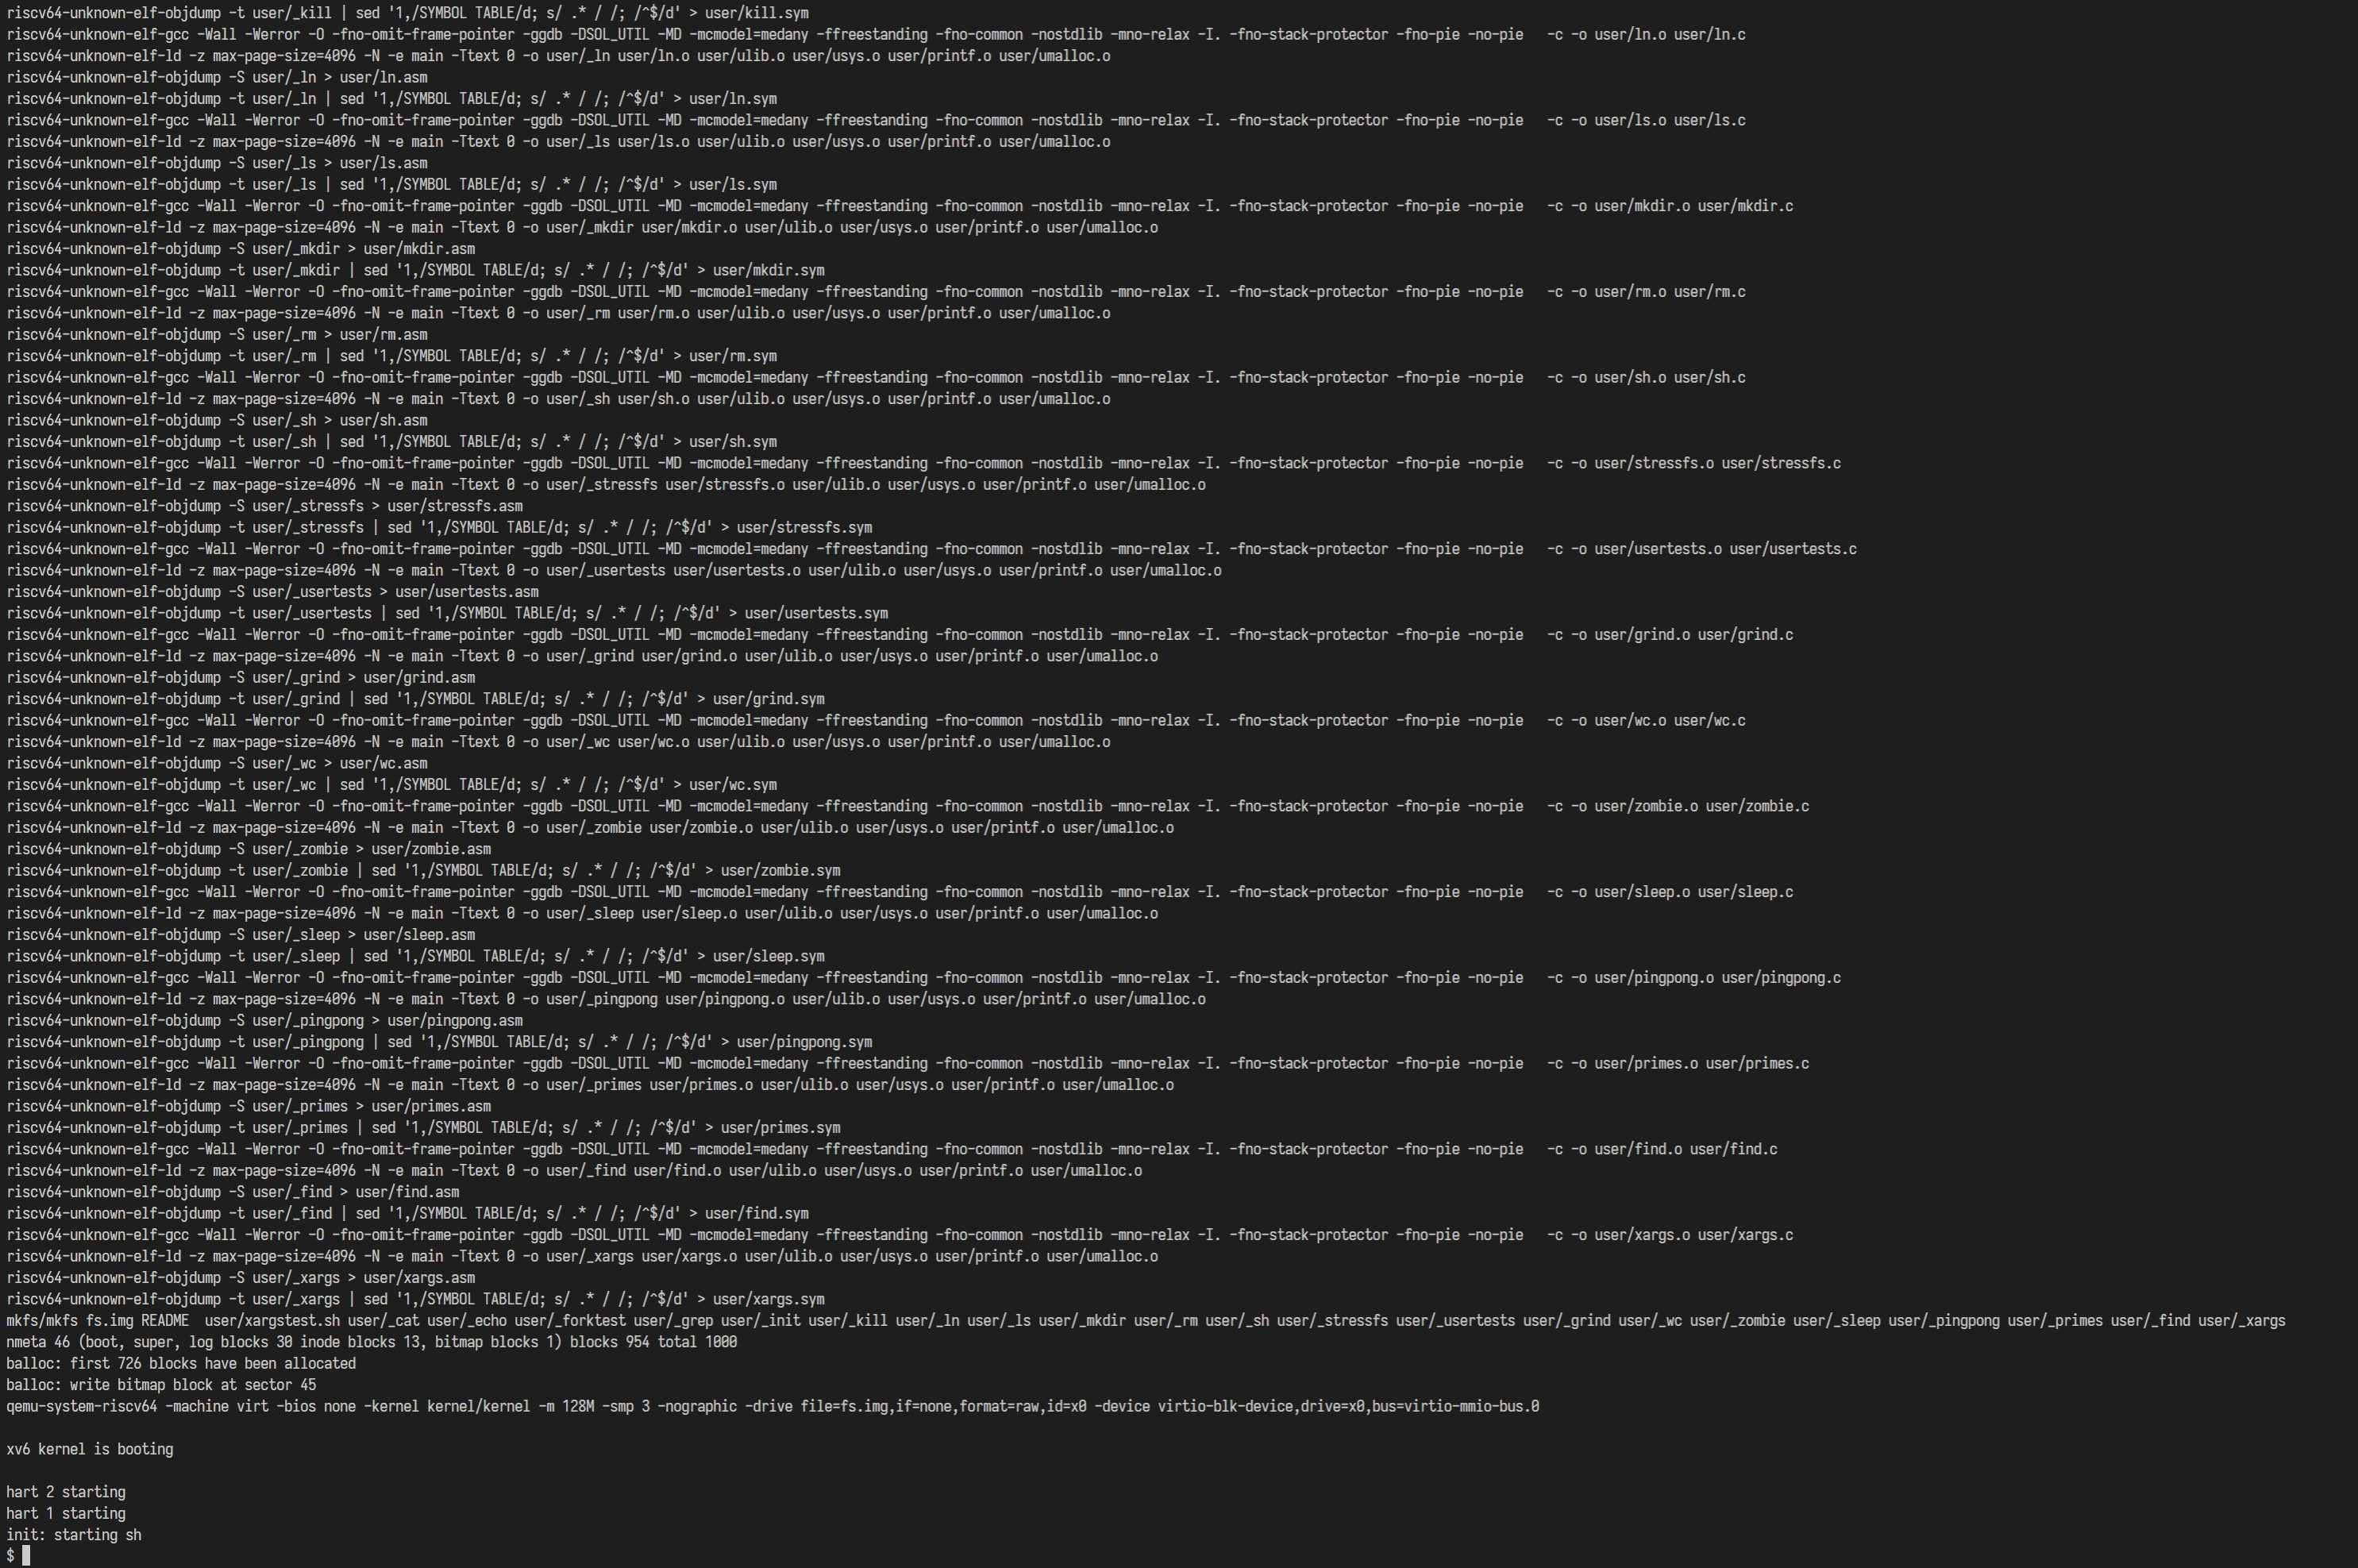
\includegraphics[width=0.7\textwidth]{boot_xv6.jpg}
  \caption{成功启动 xv6 系统的界面}
\end{figure}
xv6 启动后, init 进程会启动一个 shell 等待用户的命令。在这个简易的 shell 中,可以使用 \lstinline{ls} 指令列出根目录下的文件,然后试着执行一些内置的程序,例如执行 \lstinline{cat README} ,即可查看 README 文件的内容。

若要结束运行 xv6 并终止 qemu,需在键盘上同时按下 Ctrl+A 键,然后按下 X 键,即可终止 qemu 的运行。

\section{实现 sleep 工具}

在该实验中,我们需要实现 Unix 中经典的实用工具 sleep 。 sleep 工具的作用是等待给定的 tick 数并退出( tick 是指两次次时钟中断的间隔时间)。根据要求,我们需要将实现的源码放置在 \lstinline{user/sleep.c} 。

在开始写代码之前,我们可以先查看其它实用工具的源码,用以习惯其书写的方式。例如,打开源码 \lstinline{user/echo.c} :
\begin{lstlisting}[language=C]
#include "kernel/types.h"
#include "kernel/stat.h"
#include "user/user.h"

int
main(int argc, char *argv[])
{
  int i;

  for(i = 1; i < argc; i++){
    write(1, argv[i], strlen(argv[i]));
    if(i + 1 < argc){
      write(1, " ", 1);
    } else {
      write(1, "\n", 1);
    }
  }

  exit(0);
}
\end{lstlisting}

注意到该源码与我们日常书写的 C 语言源码大致相同,但也存在几个明显的区别:

1) include 部分引入的头文件不是标准的 C 语言库的头文件(毕竟 xv6 还没有实现标准 C 语言库);

2)程序退出时使用的是 \lstinline{exit(0);} 而非一般的 \lstinline{return 0;} 。

\begin{proposition}[为什么使用 exit 系统调用退出]
实际上,在用 gcc 为 linux 构建程序时,工具链会添加所需的 exit 调用,真正的程序执行并非从 main 函数开始,而是从工具链添加的 start 函数开始的,示意代码如下所示:
\begin{lstlisting}[language=C]
void start(void) {
    /* get argc, argv, env) */
    int r = main(argc, argv, envp);  /*  << start calls the actual main */
    exit(r);
}
\end{lstlisting}
在 xv6 中,由于我们没有这样配置工具链,故而需要手动添加 \lstinline{exit(0);} 语句。
该系统调用的作用是按照既定的步骤结束一个进程(关闭文件,释放资源,唤醒等待的父进程,修改自身状态等),具体实现参照 \lstinline{kernel/proc.c} 中的 \lstinline{void exit(int status)}。
\end{proposition}

熟悉了 \lstinline{user/echo.c} 的写法后,我们将该文件复制为 \lstinline{user/sleep.c} ,然后对其进行修改,应该就能得到所需的实用程序。为了查找我们实现 sleep 功能的系统调用,需要打开 \lstinline{user/user.h} 查看我们可以使用的一些系统调用和函数。不难发现, \lstinline{user/user.h} 中定义了如下系统调用:
\begin{lstlisting}[language=C]
  int sleep(int);
\end{lstlisting}
由于 sleep 只接受一个参数,故而我们可以简化对 \lstinline{int argc, char *argv[]} 的处理,使用 \lstinline{user/user.h} 提供的 \lstinline{int atoi(const char*)} 将第一个参数转化为整数,然后执行 \lstinline{int sleep(int)} 系统调用,最后使用 \lstinline{exit(0);} 退出进程。依据此思路写出的 \lstinline{user/sleep.c} 如下所列:
\begin{lstlisting}[language=C]
#include "kernel/types.h"
#include "kernel/stat.h"
#include "user/user.h"

int main(int argc, char *argv[])
{
    int sec;
    if (argc <= 1)
    {
        printf("usage: sleep [seconds]\n");
        exit(0);
    }
    sec = atoi(argv[1]);
    sleep(sec);
    exit(0);
}
\end{lstlisting}

在完成代码的编写后,需要将该源文件加入到 xv6 的 Makefile 里,这样工具链才会编译我们编写的用户程序。打开 \lstinline{Makefile} ,找到 \lstinline{UPROGS} 环境变量,然后按照其格式,在其后面加入一行:
\begin{lstlisting}
	$U/_sleep\
\end{lstlisting}
保存后在终端里执行 \lstinline{make qemu} ,之前编译的内核不会被重新编译,进入 xv6 后输入 \lstinline{ls} ,可以看到我们的程序已经在文件系统的根目录下了。执行 \lstinline{sleep 1000} ,其行为符合预期。

使用 xv6 实验自带的测评工具测评,在终端里输入 \lstinline{./grade-lab-util sleep} ,即可进行自动评测,如下图所示:
\begin{figure}[H]
  \centering
  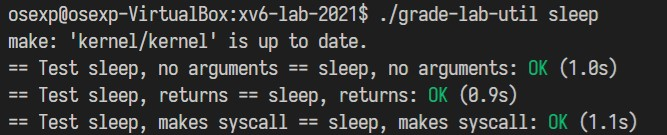
\includegraphics[width=0.8\textwidth]{util_sleep.jpg}
  \caption{ sleep 的测评结果}
\end{figure}
可见测试全部通过。

\section{实现 pingpong 工具}

在该实验中,我们需要实现一个名为 pingpong 的实用工具,用以验证 xv6 的进程通信的一些机制。该程序创建一个子进程,并使用管道与子进程通信:父进程首先发送一字节的数据给子进程,子进程接收到该数据后,在 shell 中打印 "<pid>: received ping" ,其中 pid 为子进程的进程号;子进程接收到数据后,向父进程通过管道发送一字节数据,父进程收到数据后在 shell 中打印 "<pid>: received pong" ,其中 pid 为父进程的进程号。

首先和上一个实验一样,复制一个实用程序的源码到 \lstinline{user/pingpong.c} 并且在 Makefile 中添加该程序。

在开始书写代码之前,我们需要了解实现 pingpong 所需要的系统调用:
\begin{enumerate}
  \item 用于创建管道的 pipe 系统调用
  \item 用于创建子进程的 fork 系统调用
  \item 用于读取管道的 read 系统调用
  \item 用于写管道的 write 系统调用
  \item 用于查询进程号的 getpid 系统调用
\end{enumerate}
此外,\lstinline{user/user.h} 提供了 \lstinline{void printf(const char*, ...)} 函数,用于 shell 中的格式化输出。这些系统调用和函数的作用大多可以通过查看其它已经编写好的用户程序学习,或者可以通过 xv6 的教材 \footnote{\url{https://pdos.csail.mit.edu/6.828/2021/xv6/book-riscv-rev2.pdf}} 进行学习。

根据 pingpong 程序的要求,我们需要先完成创建子进程的工作。一般而言,创建子进程的代码段如下所示:
\begin{lstlisting}[language=C]
    int pid = fork();
    if (pid == 0)
    {
      /*  child process code */
    }
    else
    {
      /*  parent process code */
    }
\end{lstlisting}

这样书写与 fork 系统调用的机制有关: fork 会将父进程的寄存器(又称为上下文)、内存空间和进程控制块复制一份,生成子进程,并且将子进程的进程控制块中的父进程指针指向其父进程;此时父子进程几乎完全一致,为了方便程序判断自己是父还是子, fork 会给两个进程不同的返回值,父进程得到的是子进程的 pid ,而子进程的返回值则为0。通过这个机制,我们便不难理解上面的代码。

在测试完成进程的创建后,我们需要设置管道。考虑到 fork 会将父进程的几乎所有内容完整地复制到子进程中(包括已经赋值完成的变量和打开的文件),我们可以在 fork 前打开两个双向管道,然后分别在父子进程中关闭两个管道的读端和写端,这样就省去了创建完子进程后再进行设置时的种种困难。

有了这些思想,便可以实现出下面的 \lstinline{user/pingpong.c} 的代码:
\begin{lstlisting}[language=C]
#include "kernel/types.h"
#include "kernel/stat.h"
#include "user/user.h"

char buf[128];

int main(int argc, char *argv[])
{
    int p1[2], p2[2], pid;
    pipe(p1);
    pipe(p2);

    if (fork() == 0)
    {
        close(p2[1]);
        close(p1[0]);
        pid = getpid();
        int num_read = read(p2[0], buf, 1);
        if (num_read == 1)
        {
            printf("%d: received ping\n", pid);
            write(p1[1], buf, 1);
        }
    }
    else
    {
        close(p1[1]);
        close(p2[0]);
        pid = getpid();
        write(p2[1], buf, 1);
        int num_read = read(p1[0], buf, 1);
        if (num_read == 1)
        {
            printf("%d: received pong\n", pid);
        }
    }

    exit(0);
}
\end{lstlisting}

保存后在终端里执行 \lstinline{make qemu} ,之前编译的内核不会被重新编译,进入 xv6 后输入 \lstinline{pingpong} ,其打印的内容符合预期。

使用 xv6 实验自带的测评工具测评,在终端里输入 \lstinline{./grade-lab-util pingpong} ,即可进行自动评测,如下图所示:
\begin{figure}[H]
  \centering
  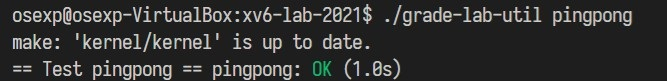
\includegraphics[width=0.8\textwidth]{util_pingpong.jpg}
  \caption{ pingpong 的测评结果}
\end{figure}
可见测试全部通过。

\begin{proposition}[管道的本质]
从我们读写管道使用的 read 和 write 系统调用中不难发现,管道本质上是一种(用于进程间通信缓冲的)特殊的文件。

现实的 Linux 系统中,有大量实用工具只从标准输入读入,并输出到标准输出。考虑到管道其实是一种特殊的文件, shell 可以通过重定向的技术,将标准输入输出重定向到管道中,从而使得这些程序可以用类似流水线的方式串联起来合作完成任务:
\begin{lstlisting}
$ ls user | grep ping
_pingpong
pingpong.asm
pingpong.c
pingpong.d
pingpong.o
pingpong.sym
\end{lstlisting}

上面的例子中,使用“|”连接两个程序: ls 的输出内容流入到管道的一端 (标准输出)。随后,内容一直流到管道的另一端 (标准输入) 由 grep 接收。由于管道本质上是文件,故只接受 byte stream,且可以作为一个固定大小的缓冲区(在 Linux 中默认为 128KB)。在 xv6 中,管道的机制也是类似的。
\end{proposition}


\section{基于管道的质数筛}

通过上面两个实验,我们已经基本熟悉了进程和管道的一些基本概念。这些概念可以帮助我们构建更加高效的、涉及多个进程的程序。一个经典的案例是 Doug McIlroy 提出的基于管道的多进程质数筛 \footnote{原文参见: \url{https://swtch.com/~rsc/thread/}}。

该质数筛的基本思路是每一个进程负责检验一个质数是否为输入的因子,在每次发现一个新质数后,就新建一个进程并令其负责检验该质因子,进程间通过管道传递数据。具体的伪代码如下:
\begin{lstlisting}
p = get a number from left neighbor
print p
loop:
    n = get a number from left neighbor
    if (p does not divide n)
        send n to right neighbor
\end{lstlisting}

最初的父进程负责产生 2 到 maxn 的整数,然后产生一个子进程用于检验质因子 2 。第一个不能被质因子整除的数用于产生下一个子进程,并输出该数,且质数筛的性质保证了该数为质数。

实现过程中,需要维护读端和写端的管道,不断读取上一个进程写入管道的内容,并在合适的条件下生成子进程并将其它数字写入管道。笔者的实现为了简洁,使用了主函数递归来避免多次的 fork 调用:
\begin{lstlisting}[language=C]
#include "kernel/types.h"
#include "kernel/stat.h"
#include "user/user.h"

const int MAX_NUM = 35;

int p1[2], fdr, fdw;
long p, n;
int is_first = 1;

int main(int argc, char *argv[])
{
    if (is_first == 1)
    {
        is_first = 0;
        pipe(p1);
        fdr = p1[0];
        fdw = p1[1];
        for (n = 2; n <= MAX_NUM; n++)
        {
            write(fdw, (void *)&n, 8);
        }
        close(fdw);
    }
    if (fork() == 0)
    {
        if (read(fdr, (void *)&p, 8))
        {
            printf("prime %d\n", p);
            pipe(p1);
            fdw = p1[1];
        }

        while (read(fdr, (void *)&n, 8))
        {
            if (n % p != 0)
                write(fdw, (void *)&n, 8);
        }
        fdr = p1[0];
        close(fdw);
        main(argc, argv);
    }
    else
    {
        wait((int *)0);
        close(fdr);
    }

    exit(0);
}
\end{lstlisting}

使用 xv6 实验自带的测评工具测评,在终端里输入 \lstinline{./grade-lab-util primes} ,即可进行自动评测,如下图所示:
\begin{figure}[H]
  \centering
  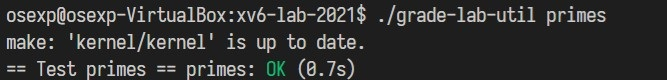
\includegraphics[width=0.8\textwidth]{util_primes.jpg}
  \caption{ primes 的测评结果}
\end{figure}
可见测试全部通过。

\paragraph*{实验结果} 在完成 Lab Utilities 中的所有实验后,根据 MIT 6.S081 的传统,需要在实验目录下创建一个名为 \lstinline{time.txt} 文本文件,其中只包含一行,为完成该实验的小时数。然后在终端中执行 \lstinline{./grade-lab-util} ,即可对整个实验进行自动评分,笔者的结果如下:
\begin{figure}[H]
  \centering
  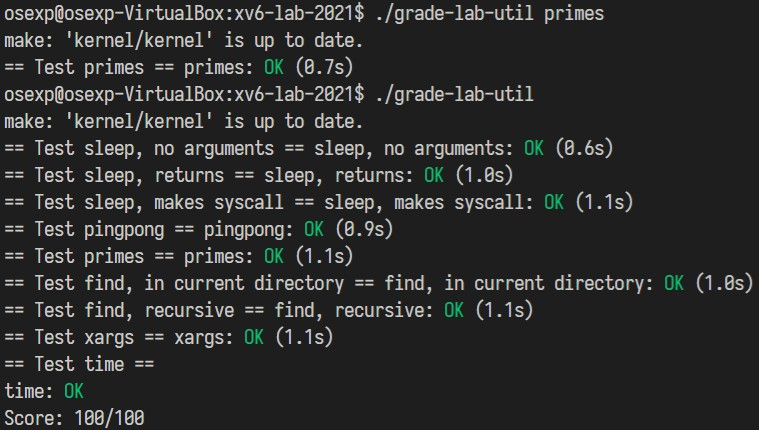
\includegraphics[width=0.8\textwidth]{util_grade.jpg}
  \caption{ Lab Utilities 的测评结果}
\end{figure}
可见测试全部通过,得分为满分。

\section{小结:进程的基本概念}

通过 Lab Utilities 中的几个实验,即便我们没有查阅或修改 xv6 的内核,只是从用户的角度使用进程,也可以如管中窥豹般看到进程的一些性质。

进程作为实例化的程序,拥有自己的地址空间和上下文。这个特点在 pingpong 实验中体现地极为明显:设置好的变量在 fork 之后被保持,且 fork 后的进程中变量的修改不影响原有进程。

进程拥有自己的地址空间和上下文的特点对于并发执行和资源分配是极其有利的,但对于进程间通信则不太友好:相比于直接使用共享内存而言,进程需要借助一种特殊的文件“管道”来进行通信。当进程创建管道时,每次都需要提供两个文件描述符来操作管道。其中一个对管道进行写操作,另一个对管道进行读操作。对管道的读写与一般的 IO 系统函数一致,使用 write 函数写入数据,使用 read 读出数据。

即便 fork 和 pipe 机制十分简明易懂,这两个机制仍然足够让我们构建高效的、涉及多个进程的并发程序。相比于单个进程,多个进程通过管道通信可以有效地利用多 CPU 系统的资源,且配合操作系统的调度可以使得 IO 效率与 CPU 利用率达到较高的水平,从而提高计算机系统的效率。
\chapter{Lab System calls:系统调用实验}
\begin{introduction}
    \item 追踪系统调用
    \item 实现 Sysinfo 系统调用
    \item 系统调用的执行过程
    \item 增加系统调用的一般步骤
\end{introduction}

在上一个实验中,我们使用操作系统提供的各类系统调用完成了复杂的任务。在 Lab System calls 的实验中,我们会深入操作系统的内核,为 xv6 的系统调用添加一些功能,乃至添加新的系统调用。

\section{追踪系统调用}

为了方便对系统调用进行 debug ,我们引入一个新的系统调用 trace ,用以追踪(打印)用户程序使用系统调用的情况。该系统调用接受一个参数,被称为 mask (掩码),用以设置被追踪的系统调用:例如,若我们想要追踪 fork 系统调用,则需要调用 \lstinline{trace(1 << SYS_fork)} ,其中 \lstinline{SYS_fork} 是 fork 系统调用的编号。该进程调用过 \lstinline{trace(1 << SYS_fork)} 后,如果该进程后续调用了 fork 系统调用,调用 fork 时内核则会打印形如 \lstinline{<pid>: syscall fork -> <ret_value>} 的信息(但无需打印传入系统调用的参数)。

该实验提供了一个用户态程序用来方便我们测试 trace 功能,该用户态程序的源码在 \lstinline{user/trace.c} 。如果我们正确实现了 trace 系统调用,则使用 trace 用户程序的情况如下面的例子所示:

\begin{lstlisting}
$ trace 2147483647 grep hello README
4: syscall trace -> 0
4: syscall exec -> 3
4: syscall open -> 3
4: syscall read -> 1023
4: syscall read -> 966
4: syscall read -> 70
4: syscall read -> 0
4: syscall close -> 0
\end{lstlisting}

这个实验需要我们着手修改 xv6 的内核,但在修改内核之前,我们需要先将 \lstinline{$U/_trace} 加入到 \lstinline{Makefile} 中的 \lstinline{UPROGS} 环境变量中。此时如果直接运行 \lstinline{make qemu} ,则会无法通过编译,原因时我们还没有将 trace 系统调用加到 xv6 的用户态库和内核中。

按照下面的步骤将 trace 系统调用加入到户态库和内核中(具体的原理将在下文的小结中讨论):
\begin{enumerate}
    \item 在 \lstinline{user/user.h} 中的系统调用部分加入一行 \lstinline{int trace(int);} 作为 trace 系统调用在用户态的入口。
    \item 在 \lstinline{user/usys.pl} 中的系统调用部分加入一行 \lstinline{entry("trace");} 用以生成调用 \lstinline{trace(int)} 入口时在用户态执行的汇编代码(这段代码被称为 stubs )。
    \item 在 \lstinline{kernel/syscall.h} 中\lstinline{#define SYS_trace  22}为 trace 分配一个系统调用的编号。
\end{enumerate}

完成上述的工作后,应当能够通过 \lstinline{make qemu} 的编译,并且进入系统。由于我们还没有真正实现 trace 系统调用,故而如果我们在 xv6 的终端中执行 \lstinline{trace 32 grep hello README},进程会因为系统报 \lstinline{unknown sys call 22} 而被终止。

接下来我们可以开始真正实现 trace 系统调用了。首先,为了保存每个进程的 trace 的参数,我们需要在进程控制块中加入一个新的变量。查看 \lstinline{kernel/proc.h} ,找到进程的数据结构 \lstinline{struct proc},在其中加入一行 \lstinline{int tracemask;},如下所示:
\begin{lstlisting}[language=C,escapechar={!}]
struct proc {
  struct spinlock lock;

  // p->lock must be held when using these:
  enum procstate state;        
  void *chan;                  
  int killed;                  
  int xstate;                  
  int pid;                     

  // wait_lock must be held when using this:
  struct proc *parent;         

  // these are private to the process, so p->lock need not be held.
  uint64 kstack;               
  uint64 sz;                   
  pagetable_t pagetable;       
  struct trapframe *trapframe; 
  struct context context;      
  struct file *ofile[NOFILE];  
  struct inode *cwd;           
  char name[16];               
  !\hl{int tracemask; }!
};
\end{lstlisting}

为了将 \lstinline{trace(int)} 的参数保存到 \lstinline{struct proc} 中,我们需要在 \lstinline{kernel/sysproc.c} 中实现 \lstinline{sys_trace(void)} 函数,代码如下:

\begin{lstlisting}[language=C,escapechar={!}]
uint64
sys_trace(void)
{
  int mask;
  argint(0, &mask);
  myproc()->tracemask = mask;
  return 0;
}
\end{lstlisting}

其中, \lstinline{argint(0, &mask);} 用于获取用户传入系统调用的第一个参数,而 \lstinline{myproc()} 则返回当前进程控制块的指针,将其 \lstinline{tracemask} 赋值为获取到的参数即可。

然后我们需要修改 \lstinline{kernel/syscall.c} 中的 \lstinline{syscall(void)} ,使其能够根据 \lstinline{tracemask} 打印所需要的信息。首先定义一个字符串常量数组,保存各系统调用的名称:
\begin{lstlisting}[language=C,escapechar={!}]
const char *syscallnames[SYS_CALL_NUM + 1] = {
    "",
    "fork",
......
......
    "trace",
};
\end{lstlisting}

然后修改 \lstinline{syscall(void)} ,在调用系统调用后,增加如下 if 语句的内容:
\begin{lstlisting}[language=C,escapechar={!}]
void syscall(void)
{
...
    p->trapframe->a0 = syscalls[num]();

    if (p->tracemask >> num & 1)
    {
      printf("%d: syscall %s -> %d\n",
             p->pid, syscallnames[num], p->trapframe->a0);
    }
...
}
\end{lstlisting}

最后,为了让 fork 后的子进程能够继承 trace 的 \lstinline{tracemask} ,需要在 \lstinline{kernel/proc.c} 中的 \lstinline{fork(void)} 中加入复制 \lstinline{tracemask} 的语句,如下面的高亮代码所示:
\begin{lstlisting}[language=C,escapechar={!}]
int fork(void)
{
  int i, pid;
  struct proc *np;
  struct proc *p = myproc();

  // Allocate process.
  if ((np = allocproc()) == 0)
  {
    return -1;
  }

  // Copy user memory from parent to child.
  if (uvmcopy(p->pagetable, np->pagetable, p->sz) < 0)
  {
    freeproc(np);
    release(&np->lock);
    return -1;
  }
  np->sz = p->sz;

  // copy saved user registers.
  *(np->trapframe) = *(p->trapframe);
  // copy trace mask
  !\hl{np->tracemask = p->tracemask;}!
  // Cause fork to return 0 in the child.
  np->trapframe->a0 = 0;
  // increment reference counts on open file descriptors.
  for (i = 0; i < NOFILE; i++)
    if (p->ofile[i])
      np->ofile[i] = filedup(p->ofile[i]);
  np->cwd = idup(p->cwd);
  safestrcpy(np->name, p->name, sizeof(p->name));
  pid = np->pid;

  release(&np->lock);

  acquire(&wait_lock);
  np->parent = p;
  release(&wait_lock);

  acquire(&np->lock);
  np->state = RUNNABLE;
  release(&np->lock);

  return pid;
}
\end{lstlisting}


此时 trace 系统调用实现完成,编译并启动 xv6 后,在 shell 中运行 \lstinline{trace 32 grep hello README} ,即可看到预期的输出。

使用 xv6 实验自带的测评工具测评,在终端里输入 \lstinline{./grade-lab-syscall trace} ,即可进行自动评测,如下图所示:
\begin{figure}[H]
  \centering
  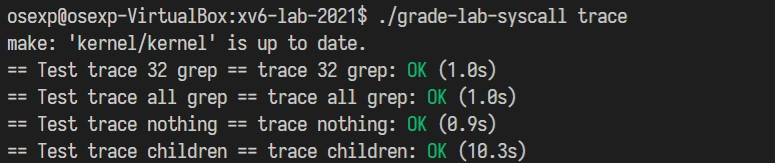
\includegraphics[width=0.8\textwidth]{syscall_trace.jpg}
  \caption{ trace 的测评结果}
\end{figure}
可见测试全部通过。

\section{实现 Sysinfo 系统调用}

常见的操作系统都会提供一些系统调用来帮助应用程序获取关于系统的信息,因而我们也被要求实现一个 sysinfo 系统调用,用于获取 xv6 运行时的信息。具体来说, xv6 已经为我们定义好了一个结构体 \lstinline{struct sysinfo} (在源码 \lstinline{kernel/sysinfo.h} )中,我们的 sysinfo 系统调用接受一个参数,即指向该结构体的指针,然后将对应的内容填入该结构体( \lstinline{freemem} 字段填写空闲的内存空间字节数, \lstinline{nproc} 字段填写状态为未使用( \lstinline{UNUSED} )的进程数)。 为了方便测试, xv6 还提供了一个用户程序 \lstinline{sysinfotest} ,当通过所有测试时该程序输出 \lstinline{sysinfotest: OK} 。

首先和上面类似,修改 \lstinline{Makefile} 中的 \lstinline{UPROGS} 环境变量,将 \lstinline{$U/_sysinfotest} 加入到其中。然后按照上面的流程添加 sysinfo 系统调用的入口,接着在 \lstinline{user/user.h} 中添加 \lstinline{struct sysinfo} 的声明:
\begin{lstlisting}[language=C,escapechar={!}]
    struct sysinfo;
    int sysinfo(struct sysinfo *);
\end{lstlisting}
然后可以通过编译。

为了获得空闲内存大小,我们需要在 \lstinline{kernel/kalloc.c} 实现一个函数。由于 xv6 管理内存空闲空间使用的是空闲链表,参照链表的结构后,只需遍历链表并计算数量,然后乘以页面大小即可。笔者的实现如下:
\begin{lstlisting}[language=C,escapechar={!}]
// Return the amount of free memory.
int getfreemem(void)
{
  int count = 0;
  struct run *r;

  acquire(&kmem.lock);
  r = kmem.freelist;
  while (r)
  {
    count++;
    r = r->next;
  }
  release(&kmem.lock);
  return count * PGSIZE;
}
\end{lstlisting}
\begin{theorem}[注意加锁] 
    当访问内核态的空闲链表时,由于可能出现并发读写的情况,故而我们需要先获取该数据结构的锁,然后再进行读取,最后释放该锁;否则可能读到“脏”的数据。使用下面的代码进行锁的获取和释放:
\begin{lstlisting}[language=C,escapechar={!}]   
acquire(&kmem.lock);
......
release(&kmem.lock);
\end{lstlisting}
\end{theorem}

统计空闲进程控制块的数量的函数的实现也类似,只是进程控制块是用静态数组管理的,故而只需要用一个循环遍历该数组即可。笔者在 \lstinline{kernel/proc.c} 中的实现如下:
\begin{lstlisting}[language=C]
// Return the number of non-UNUSED procs in the process table.
int getnproc(void)
{
  struct proc *p;
  int count = 0;
  for (p = proc; p < &proc[NPROC]; p++)
  {
    acquire(&p->lock);
    if (p->state != UNUSED)
    {
      count++;
      release(&p->lock);
    }
    else
    {
      release(&p->lock);
    }
  }
  return count;
}
\end{lstlisting}
\begin{theorem}[同样注意加锁] 
    访问内核态的数据结构时,谨慎起见总是要加锁。
\end{theorem}

由于虚拟存储机制的存在,内核态的页表与用户态的页表不同,而用户传入的地址是用户态的地址,故而剩下的问题就在于如何将内核态的数据复制到用户态的数据结构中。根据 xv6 实验手册 \footnote{\url{https://pdos.csail.mit.edu/6.828/2021/labs/syscall.html}} 的提醒,我们需要参考 \lstinline{kernel/sysfile.c} 中 \lstinline{sys_fstat()} 和 \lstinline{kernel/file.c} 中 \lstinline{filestat()} 的实现。在 \lstinline{filestat()} 中,有一行代码至关重要(下面高亮的一行):
\begin{lstlisting}[language=C,escapechar={!}]
// Get metadata about file f.
// addr is a user virtual address, pointing to a struct stat.
int
filestat(struct file *f, uint64 addr)
{
  struct proc *p = myproc();
  struct stat st;
  
  if(f->type == FD_INODE || f->type == FD_DEVICE){
    ilock(f->ip);
    stati(f->ip, &st);
    iunlock(f->ip);
    !\hl{if(copyout(p->pagetable, addr, (char *)\&st, sizeof(st)) < 0)}!
      return -1;
    return 0;
  }
  return -1;
}
\end{lstlisting}

此处的 \lstinline{copyout(p->pagetable, addr, (char *)&st, sizeof(st))} 接受进程的页表,并将内核态中的一段数据拷贝到进程内存空间中的地址处。有了这个函数,我们也可以用相同的方法将 \lstinline{struct sysinfo} 拷贝到用户态进程中,笔者在 \lstinline{kernel/sysproc.c} 中实现的 \lstinline{sys_sysinfo(void)} 如下所示:
\begin{lstlisting}[language=C]
extern int getnproc(void);
extern int getfreemem(void);
uint64
sys_sysinfo(void)
{
  struct proc *p = myproc();
  struct sysinfo st;
  uint64 addr; // user pointer to struct stat
  st.freemem = getfreemem();
  st.nproc = getnproc();
  if (argaddr(0, &addr) < 0)
    return -1;
  if (copyout(p->pagetable, addr, (char *)&st, sizeof(st)) < 0)
    return -1;
  return 0;
}
\end{lstlisting}

此时 sysinfo 系统调用实现完成,编译并启动 xv6 后,在 shell 中运行 \lstinline{sysinfotest} ,即可看到预期的输出:
\begin{lstlisting}
$ sysinfotest
sysinfotest: start
sysinfotest: OK
$ 
\end{lstlisting}

使用 xv6 实验自带的测评工具测评,在终端里输入 \lstinline{./grade-lab-syscall sysinfo} ,即可进行自动评测,如下图所示:
\begin{figure}[H]
  \centering
  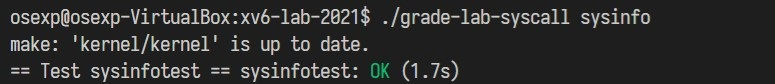
\includegraphics[width=0.8\textwidth]{syscall_sysinfo.jpg}
  \caption{ sysinfo 的测评结果}
\end{figure}
可见测试全部通过。

\paragraph*{实验结果} 在完成 Lab System calls 中的所有实验后,根据 MIT 6.S081 的传统,需要在实验目录下创建一个名为 \lstinline{time.txt} 文本文件,其中只包含一行,为完成该实验的小时数。然后在终端中执行 \lstinline{./grade-lab-syscall} ,即可对整个实验进行自动评分,笔者的结果如下:
\begin{figure}[H]
  \centering
  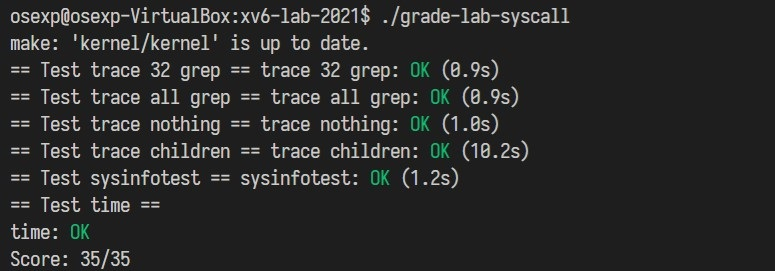
\includegraphics[width=0.8\textwidth]{syscall_grade.jpg}
  \caption{ Lab System calls 的测评结果}
\end{figure}
可见测试全部通过,得分为满分。

\section{小结:系统调用的执行过程}

通过上面的两个实验,我们能够大致了解一个系统调用发生的全过程。但实际上,上面的两个实验涉及到的内容并不细致,在这里笔者会以 sleep 系统调用为例,详细总结一个系统调用发生的各个阶段及其相关的细节。

首先准备实验环境,我们先从 \url{https://github.com/mit-pdos/xv6-riscv.git} 克隆下一个干净的 xv6 源码库,然后编写一个简单的 \lstinline{user/sleep.c},如下所示:
\begin{lstlisting}[language=C]
#include "kernel/types.h"
#include "kernel/stat.h"
#include "user/user.h"

int
main(int argc, char *argv[])
{
  sleep(10);
  exit(0);
}
\end{lstlisting}

将 \lstinline{$U/_sleep} 加入到 \lstinline{Makefile} 中的 \lstinline{UPROGS} 环境变量中,然后使用 \lstinline{make} 编译整个源码库。编译后除了会产生二进制文件外, xv6 的 \lstinline{Makefile} 还十分贴心地为我们生成了反汇编后的 \lstinline{user/sleep.asm} 文件,浏览该文件,可以看到如下的内容:
\begin{lstlisting}
user/_sleep:     file format elf64-littleriscv


Disassembly of section .text:

0000000000000000 <main>:
#include "kernel/stat.h"
#include "user/user.h"

int
main(int argc, char *argv[])
{
   0:	1141                	addi	sp,sp,-16
   2:	e406                	sd	ra,8(sp)
   4:	e022                	sd	s0,0(sp)
   6:	0800                	addi	s0,sp,16
  sleep(10);
   8:	4529                	li	a0,10
   a:	00000097          	auipc	ra,0x0
   e:	318080e7          	jalr	792(ra) # 322 <sleep>
  exit(0);
  12:	4501                	li	a0,0
  14:	00000097          	auipc	ra,0x0
  18:	27e080e7          	jalr	638(ra) # 292 <exit>
......
\end{lstlisting}
重点关注 \lstinline{sleep(10);} 的反汇编代码:
\begin{lstlisting}
......
  sleep(10);
   8:	4529                li	a0,10
   a:	00000097          	auipc	ra,0x0
   e:	318080e7          	jalr	792(ra) # 322 <sleep>
......
\end{lstlisting}

根据 RISC-V ABI ,寄存器 a0 用于存储函数的传入参数和返回值,故而该程序将立即数 10 加载到 a0 中,然后利用 \lstinline{auipc} 和 \lstinline{jalr} 两条指令跳转至 sleep 系统调用的函数体中。由于 \lstinline{jalr} 指令旁边的注释已经给出了 sleep 调用的地址,我们从该地址开始看:
\begin{lstlisting}
......
0000000000000322 <sleep>:
.global sleep
sleep:
 li a7, SYS_sleep
 322:	48b5                	li	a7,13
 ecall
 324:	00000073          	ecall
 ret
 328:	8082                	ret
......
\end{lstlisting}

这段代码即是 \lstinline{user/usys.S} 经汇编和链接后生成的代码,其中, \lstinline{li	a7,13} 将 sleep 的系统调用编号 13 载入到 a7 寄存器,此时的 a0 寄存器中仍然保存着我们传入 sleep 的参数 10 。然后程序执行 \lstinline{ecall} 进入内核态。下图展示了 \lstinline{ecall} 指令的机制\footnote{图片摘录自:\url{https://jborza.com/post/2021-04-21-ecalls-and-syscalls/}}:
\begin{figure}[H]
  \centering
  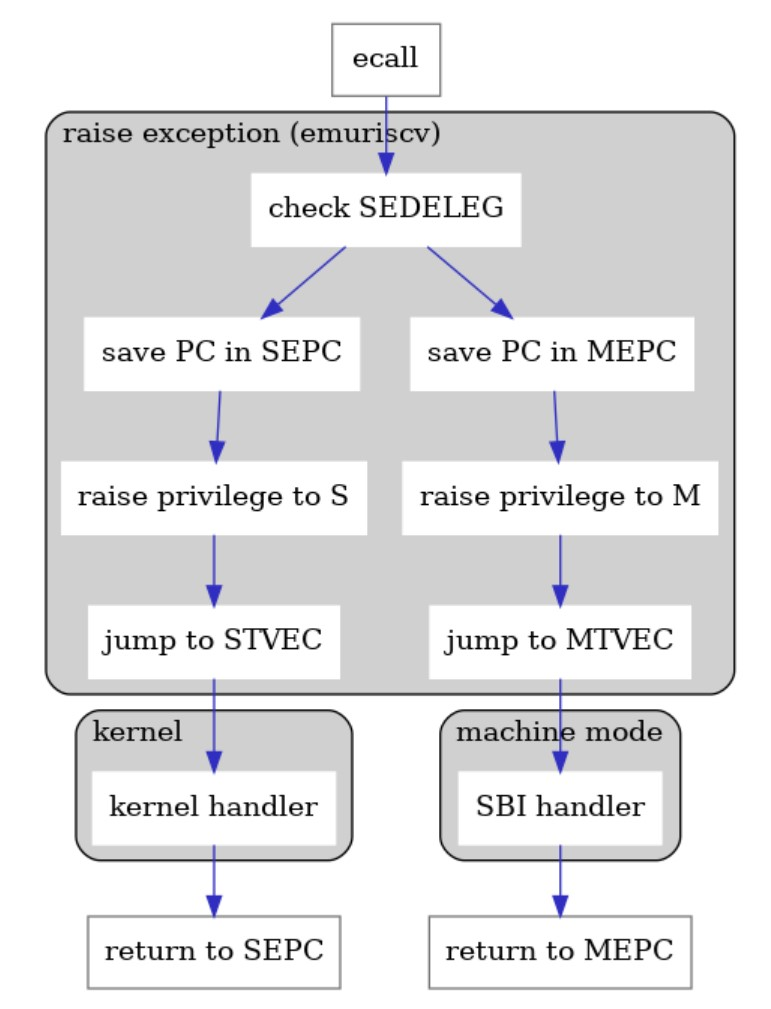
\includegraphics[width=0.6\textwidth]{syscall_ecall.jpg}
  \caption{ ecall 指令的机制}
\end{figure}

此时机器执行的是左侧的路径,即将当前的程序计数器 PC 保存到 SEPC 寄存器中,然后提升处理器的工作权限并跳转至 STVEC 所指向的代码处执行。此时 STVEC 所指向的代码即为 \lstinline{kernel/trampoline.S} 中的 \lstinline{.globl uservec},这段汇编代码保存用户态程序的各种寄存器到其 trapframe 中(此时的用户态程序便不再执行),恢复内核态的栈指针和页表,并跳转至 \lstinline{kernel/trap.c} 中的 \lstinline{usertrap(void)} 继续完成内核态的工作。

在 \lstinline{usertrap(void)} 中,获取了当前进程的控制块 \lstinline{struct proc *p = myproc();} 后,首先需要保存 \lstinline{ecall} 时保存到 SPEC 寄存器中的用户态 PC ,然后判断中断的种类。由 \lstinline{ecall} 引发的调用 syscall 的中断会使得 SCAUSE 的值被设为 8 ,故而会执行下面分支中的语句:
\begin{lstlisting}[language=C]
......
if(r_scause() == 8){
    // system call

    if(p->killed)
      exit(-1);

    // sepc points to the ecall instruction,
    // but we want to return to the next instruction.
    p->trapframe->epc += 4;

    // an interrupt will change sstatus &c registers,
    // so don't enable until done with those registers.
    intr_on();

    syscall();
......
\end{lstlisting}

该过程主要是将 trapframe 中保存的用户 PC 加 4 ,即指向 \lstinline{ecall} 的下一个指令,开启中断,并调用内核中系统调用的入口 \lstinline{syscall()} 。该入口在 \lstinline{kernel/syscall.c} 中被实现:
\begin{lstlisting}[language=C]
void
syscall(void)
{
  int num;
  struct proc *p = myproc();

  num = p->trapframe->a7;
  if(num > 0 && num < NELEM(syscalls) && syscalls[num]) {
    p->trapframe->a0 = syscalls[num]();
  } else {
    printf("%d %s: unknown sys call %d\n",
            p->pid, p->name, num);
    p->trapframe->a0 = -1;
  }
}
\end{lstlisting}

该函数获取了当前进程的控制块 \lstinline{struct proc *p = myproc();} 后,读取该进程企图调用的系统调用的编号:该编号在 \lstinline{user/usys.S} 中被放入 a7 寄存器中,然后 \lstinline{trampoline.S} 中的 \lstinline{uservec} 过程将 a7 寄存器中的值保存到了进程的 trapframe 中,此时使用 \lstinline{num = p->trapframe->a7;} 将其读出,稍作检查即可使用函数指针调用对应的实现。在本例子中,由于系统编号为 13 ,故调用的确实是 \lstinline{sys_sleep}:
\begin{lstlisting}[language=C]
uint64
sys_sleep(void)
{
  int n;
  uint ticks0;

  if(argint(0, &n) < 0)
    return -1;
  acquire(&tickslock);
  ticks0 = ticks;
  while(ticks - ticks0 < n){
    if(myproc()->killed){
      release(&tickslock);
      return -1;
    }
    sleep(&ticks, &tickslock);
  }
  release(&tickslock);
  return 0;
}
\end{lstlisting}

注意到在 \lstinline{kernel/sysproc.c} 中实现的 \lstinline{uint64 sys_sleep(void)} 并不接受参数,那之前用户态程序的参数如何传入到系统调用中呢?事实上,用户态程序将系统调用的参数保存在了 a0 ~ a5 着几个寄存器中,而这些寄存器在 \lstinline{uservec} 过程中都被保存到了进程的 trapframe 中(即都在内存中的进程控制块相关的数据结构中),故而只需要读取 trapframe 中对应的寄存器即可获得参数。读取寄存器的过程由一系列函数完成,如 \lstinline{int argint(int n, int *ip)} 、 \lstinline{static uint64 argraw(int n)} 等。

当 \lstinline{sys_sleep()} 完成了其工作后,返回至 \lstinline{syscall()} ,进而返回至 \lstinline{kernel/trap.c} 中的 \lstinline{usertrap(void)} ,此时执行 \lstinline{usertrapret();} 用于完成返回到用户态的工作:
\begin{lstlisting}[language=C]
void
usertrapret(void)
{
  struct proc *p = myproc();

  // we're about to switch the destination of traps from
  // kerneltrap() to usertrap(), so turn off interrupts until
  // we're back in user space, where usertrap() is correct.
  intr_off();

  // send syscalls, interrupts, and exceptions to trampoline.S
  w_stvec(TRAMPOLINE + (uservec - trampoline));

  // set up trapframe values that uservec will need when
  // the process next re-enters the kernel.
  p->trapframe->kernel_satp = r_satp();         // kernel page table
  p->trapframe->kernel_sp = p->kstack + PGSIZE; // process's kernel stack
  p->trapframe->kernel_trap = (uint64)usertrap;
  p->trapframe->kernel_hartid = r_tp();         // hartid for cpuid()

  // set up the registers that trampoline.S's sret will use
  // to get to user space.
  
  // set S Previous Privilege mode to User.
  unsigned long x = r_sstatus();
  x &= ~SSTATUS_SPP; // clear SPP to 0 for user mode
  x |= SSTATUS_SPIE; // enable interrupts in user mode
  w_sstatus(x);

  // set S Exception Program Counter to the saved user pc.
  w_sepc(p->trapframe->epc);

  // tell trampoline.S the user page table to switch to.
  uint64 satp = MAKE_SATP(p->pagetable);

  // jump to trampoline.S at the top of memory, which 
  // switches to the user page table, restores user registers,
  // and switches to user mode with sret.
  uint64 fn = TRAMPOLINE + (userret - trampoline);
  ((void (*)(uint64,uint64))fn)(TRAPFRAME, satp);
}
\end{lstlisting}


为了返回用户态, \lstinline{usertrapret();} 需要在关闭中断的条件下设置好进程的 trapframe 中的各数据项供 \lstinline{kernel/trampoline.S} 中的 \lstinline{uservec} 下次使用,然后还需要设置好处理器的工作模式、页表地址和用户态 PC ,最后使用函数指针的方式调用 \lstinline{kernel/trampoline.S} 中的 \lstinline{userret} ,恢复各寄存器,然后使用 \lstinline{sret} 指令回到用户态,并从用户态 PC 处开始执行。

此时的用户态程序从 \lstinline{ecall} 的下一个指令开始执行,恍如从一场梦中醒来,系统调用已经做完了其需要的事情。用户程序无法发觉操作系统内核进行了什么工作,颇有“地上一日,天上一年”的味道。

几乎所有的系统调用都与上面的过程类似,只有在内核态进行的工作有所不同。有一些涉及用户线程的系统调用(例如后文的定时器 alarm 系统调用),在返回用户态前会修改进程执行的上下文,但其返回用户态的工作总是由 \lstinline{kernel/trampoline.S} 中的 \lstinline{userret} 进行的。

\section{小结:增加系统调用的一般步骤}

通过上文对于系统调用执行过程的小结,我们很自然地能得出添加系统调用的一般步骤:
\begin{enumerate}
    \item 在 \lstinline{user/user.h} 中的系统调用部分加入系统调用在用户态的入口。
    \item 在 \lstinline{user/usys.pl} 中的系统调用部分加入在用户态执行的汇编代码( stubs )。
    \item 在 \lstinline{kernel/syscall.h} 中为系统调用分配一个系统调用的编号。
    \item 在内核代码中实现系统调用,包括设计对应的数据结构和函数等。
\end{enumerate}
从这个实验开始,我们便有能力对 xv6 的内核进行深度的改进,并在为其添加更多的特性的过程中学习现代操作系统的诸多概念。
\chapter{Lab Page tables:页表实验}
\begin{introduction}
    \item 使用页表机制加速系统调用
    \item 打印页表
    \item 追踪被访问的页
    \item RISC-V 的页表机制
\end{introduction}

在上一个实验中,我们初次修改 xv6 的内核,为其添加了两个系统调用。本次实验的重点则是在于操作系统的另一个机制:页表。在本次实验中,我们会初探页表的一些性质,并利用页表机制完成一些任务。

\section{使用页表机制加速系统调用}

在现实的操作系统中,很多系统调用只是读取内核态的一些数据结构,而并不进行写入操作,这类系统调用的一个典型例子就是 getpid 系统调用。对于这类系统调用,诸如 Linux 等操作系统不会将内核的数据结构复制到用户空间,而是直接将存放该数据结构的页通过页表的机制映射到用户空间的对应位置,从而免去了复制的开销,提高了系统的性能。

本实验中,需要在进程创建时将一个内存页面以只读权限映射到 \lstinline{USYSCALL} 位置(参见 \lstinline{memlayout.h})中的定义。该映射的页面开头存储有内核数据结构 \lstinline{struct usyscall} ,该数据结构在进程创建时被初始化,并且存储有该进程的 pid 。在这个实验中,我们使用纯用户空间的函数 \lstinline{ugetpid()} 来替代需要进行内核态到用户态拷贝的 getpid 系统调用。户空间的函数 \lstinline{ugetpid()} 已经在用户空间中被实现了,我们需要做的是将映射页面的工作完成。

由于需要在创建进程时完成页面的映射,故而我们考虑修改 \lstinline{kernel/proc.c} 中的 \lstinline{proc_pagetable(struct proc *p)} ,即用于为新创建的进程分配页面的函数。在 \lstinline{proc_pagetable()} 完成分配新的页面后,即可以使用 \lstinline{mappages} 函数分配页面:
\begin{lstlisting}[language=C]
pagetable_t
proc_pagetable(struct proc *p)
{
  pagetable_t pagetable;

  // An empty page table.
  pagetable = uvmcreate();
  if(pagetable == 0)
    return 0;

  //map a user read only page at USYSCALL, for optimization for the getpid()
  if(mappages(pagetable, USYSCALL, PGSIZE,
              (uint64)(p->usyscall), PTE_R | PTE_U) < 0){
    uvmfree(pagetable, 0);
    return 0;
  }
......
\end{lstlisting}

页面映射时,需要设定其权限为只读,故权限位为 \lstinline{PTE_R | PTE_U} ,此后在 \lstinline{allocproc()} 中添加初始化该页面,向其中写入数据结构的代码:
\begin{lstlisting}[language=C]
......
  // Allocate a usyscall page.
  if((p->usyscall = (struct usyscall *)kalloc()) == 0){
    freeproc(p);
    release(&p->lock);
    return 0;
  }
  p->usyscall->pid = p->pid;
......
\end{lstlisting}
\begin{theorem}[注意加锁] 
    当在内核态下操作进程相关的数据结构时,由于可能出现并发读写的情况,故而我们需要先获取该数据结构的锁,然后再进行操作,最后释放该锁;否则可能造成竞争读写,导致数据不一致的情况出现。
\end{theorem}

在完成页面的初始化后,进程应当得以正常运行,但需要记得在进程结束后释放分配的页面,该动作在 \lstinline{freeproc()} 中进行,添加的代码如下:
\begin{lstlisting}[language=C]
......
  if(p->usyscall)
    kfree((void*)p->usyscall);
  p->usyscall = 0;
......
\end{lstlisting}

当考虑好进程的页面分配,页面初始化和页面回收后,映射页面的工作就全部完成了。编译并启动 xv6 后,在 shell 中运行 \lstinline{pgtbltest} ,即可看到预期的输出:
\begin{lstlisting}
$ pgtbltest
ugetpid_test starting
ugetpid_test: OK
......
\end{lstlisting}

\section{打印页表}

为了方便将页表的内容可视化,我们需要实现一个名为 \lstinline{vmprint()} 的函数,其接受一个 \lstinline{pagetable_t} 类型的参数,并按下面的格式打印页表:
\begin{lstlisting}
page table 0x0000000087f6e000
 ..0: pte 0x0000000021fda801 pa 0x0000000087f6a000
 .. ..0: pte 0x0000000021fda401 pa 0x0000000087f69000
 .. .. ..0: pte 0x0000000021fdac1f pa 0x0000000087f6b000
 .. .. ..1: pte 0x0000000021fda00f pa 0x0000000087f68000
 .. .. ..2: pte 0x0000000021fd9c1f pa 0x0000000087f67000
 ..255: pte 0x0000000021fdb401 pa 0x0000000087f6d000
 .. ..511: pte 0x0000000021fdb001 pa 0x0000000087f6c000
 .. .. ..509: pte 0x0000000021fdd813 pa 0x0000000087f76000
 .. .. ..510: pte 0x0000000021fddc07 pa 0x0000000087f77000
 .. .. ..511: pte 0x0000000020001c0b pa 0x0000000080007000
\end{lstlisting}

实现了 \lstinline{vmprint()} 之后,我们可以在 \lstinline{kernel/exec.c} 中的 \lstinline{exec()} 函数的 \lstinline{return argc} 前加入 \lstinline{if(p->pid==1) vmprint(p->pagetable)} ,即可打印 pid 为 1 的进程的页表。

为了方便使用其它与页表相关的函数,我们在 \lstinline{kernel/vm.c} 中实现 \lstinline{vmprint()} 函数。在实现该函数前,我们根据 xv6 实验手册的提示,首先阅读 \lstinline{freewalk} 函数的实现以供参考:
\begin{lstlisting}[language=C]
// Recursively free page-table pages.
// All leaf mappings must already have been removed.
void
freewalk(pagetable_t pagetable)
{
  // there are 2^9 = 512 PTEs in a page table.
  for(int i = 0; i < 512; i++){
    pte_t pte = pagetable[i];
    if((pte & PTE_V) && (pte & (PTE_R|PTE_W|PTE_X)) == 0){
      // this PTE points to a lower-level page table.
      uint64 child = PTE2PA(pte);
      freewalk((pagetable_t)child);
      pagetable[i] = 0;
    } else if(pte & PTE_V){
      panic("freewalk: leaf");
    }
  }
  kfree((void*)pagetable);
}
\end{lstlisting}

不难发现,该函数通过递归的方式逐层释放页表。仿照这种递归方式,对该函数略做修改,我们可以构造遍历页表并按层数格式打印的函数 \lstinline{vmprintwalk(pagetable_t pagetable, int depth)} :
\begin{lstlisting}[language=C]
void
vmprintwalk(pagetable_t pagetable, int depth)
{
  // there are 2^9 = 512 PTEs in a page table.
  for(int i = 0; i < 512; i++){
    pte_t pte = pagetable[i];
    if((pte & PTE_V) && (pte & (PTE_R|PTE_W|PTE_X)) == 0){
      // this PTE points to a lower-level page table.
      for (int n = 0; n < depth; n++)
        printf(" ..");
      printf("%d: pte %p pa %p\n", i, pte, PTE2PA(pte));
      uint64 child = PTE2PA(pte);
      vmprintwalk((pagetable_t)child, depth+1);
    } else if(pte & PTE_V){
      for (int n = 0; n < depth; n++)
        printf(" ..");
      printf("%d: pte %p pa %p\n", i, pte, PTE2PA(pte));
    }
  }
}
\end{lstlisting}

然后实现 \lstinline{vmprint()} 函数时,只需给定初始深度为 1 ,调用 \lstinline{vmprintwalk(pagetable_t, int)} 即可:
\begin{lstlisting}[language=C]
void
vmprint(pagetable_t pagetable)
{
  printf("page table %p\n",pagetable);
  vmprintwalk(pagetable,1);
}
\end{lstlisting}

最后按照要求在 \lstinline{kernel/exec.c} 中的 \lstinline{exec()} 函数的 \lstinline{return argc} 前加入 \lstinline{if(p->pid==1) vmprint(p->pagetable)} :
\begin{lstlisting}[language=C]
......
    if(p->pid==1) vmprint(p->pagetable);
    return argc; // this ends up in a0, the first argument to main(argc, argv)
......
\end{lstlisting}

编译并启动 xv6 后 ,即可看到预期的输出,如下图所示:
\begin{figure}[H]
  \centering
  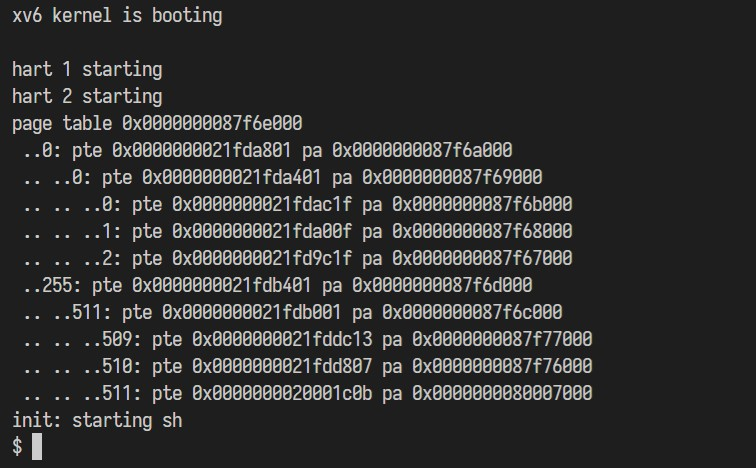
\includegraphics[width=0.8\textwidth]{pgtbl_vmprint.jpg}
  \caption{ \lstinline{vmprint()} 的输出结果}
\end{figure}

\section{追踪被访问的页}

现代很多编程语言都具备了内存垃圾回收的功能( GC , garbage collect ),而垃圾回收器功能的实现则需要得到一个页面自上次检查后是否被访问的信息。实现这种功能可以是纯软件的,但其效率低下;而利用页表的硬件机制(访问位)和操作系统相结合,在 xv6 中添加一个系统调用 \lstinline{pgaccess()} 用以读取页表的访问位并传递给用户态程序,从而告知他们一些内存页面自上次检查以来的访问情况,是一个较好的方法。

我们需要实现的 \lstinline{pgaccess()} 系统调用接受 3 个参数:第一个参数为需要检查页面的初始地址,第二个参数是从初始地址向后检查多少个页面,第三个参数则是一个指针,指向用于存储结果的位向量的首地址。

首先,按照前文提及的方法添加系统调用以及其在 \lstinline{kernel/sysproc.c} 中的实现 \lstinline{sys_pgaccess()} ,并使用 \lstinline{argint()} 和 \lstinline{argaddr()} 获取传入的参数:
\begin{lstlisting}[language=C]
int sys_pgaccess(void)
{
  uint64 srcva, st;
  int len;
  uint64 buf = 0;
  struct proc *p = myproc();

  acquire(&p->lock);

  argaddr(0, &srcva);
  argint(1, &len);
  argaddr(2, &st);
  ......
  return 0;
}
\end{lstlisting}

之后,对获取的参数进行预处理后,对每个需要检查的页面,使用 \lstinline{kernel/vm.c} 中提供的 \lstinline{walk(pagetable_t, uint64, int)} 来获取其页表项,重置该页表的 \lstinline{PTE_A} 访问位,并使用位运算将其访问状态置入临时位向量中;最后将临时位向量拷贝至用户内存空间指定的地址中。笔者的完整的实现如下:
\begin{lstlisting}[language=C]
extern pte_t *walk(pagetable_t, uint64, int);
int sys_pgaccess(void)
{
  // lab pgtbl: your code here.
  uint64 srcva, st;
  int len;
  uint64 buf = 0;
  struct proc *p = myproc();

  acquire(&p->lock);

  argaddr(0, &srcva);
  argint(1, &len);
  argaddr(2, &st);
  if ((len > 64) || (len < 1))
    return -1;
  pte_t *pte;
  for (int i = 0; i < len; i++)
  {
    pte = walk(p->pagetable, srcva + i * PGSIZE, 0);
    if(pte == 0){
      return -1;
    }
    if((*pte & PTE_V) == 0){
      return -1;
    }
    if((*pte & PTE_U) == 0){
      return -1;
    }
    if(*pte & PTE_A){
      *pte = *pte & ~PTE_A;
      buf |= (1 << i);  
    }
  }
  release(&p->lock);
  copyout(p->pagetable, st, (char *)&buf, ((len -1) / 8) + 1);
  return 0;
}
\end{lstlisting}

\begin{theorem}[再次提醒加锁] 
    页表也是内核数据结构,可能被多个处理器同时操作,故记得加锁。
\end{theorem}

至此, \lstinline{pgaccess()} 系统调用实现完成。编译并启动 xv6 后,在 shell 中运行 \lstinline{pgtbltest} ,即可看到预期的输出,如下图所示:
\begin{figure}[H]
  \centering
  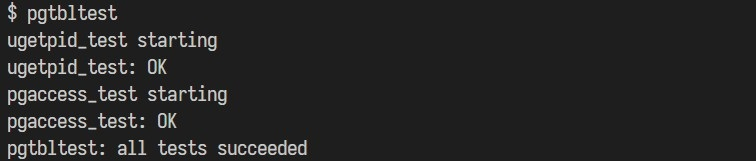
\includegraphics[width=0.8\textwidth]{pgtbl_pgaccess.jpg}
  \caption{ pgaccess 的测评结果}
\end{figure}

\paragraph*{实验结果} 在完成 Lab Page tables 中的所有实验后,根据 MIT 6.S081 的传统,需要在实验目录下创建一个名为 \lstinline{time.txt} 文本文件,其中只包含一行,为完成该实验的小时数。然后在终端中执行 \lstinline{make grade} ,即可对整个实验进行自动评分,笔者的结果如下:
\begin{figure}[H]
  \centering
  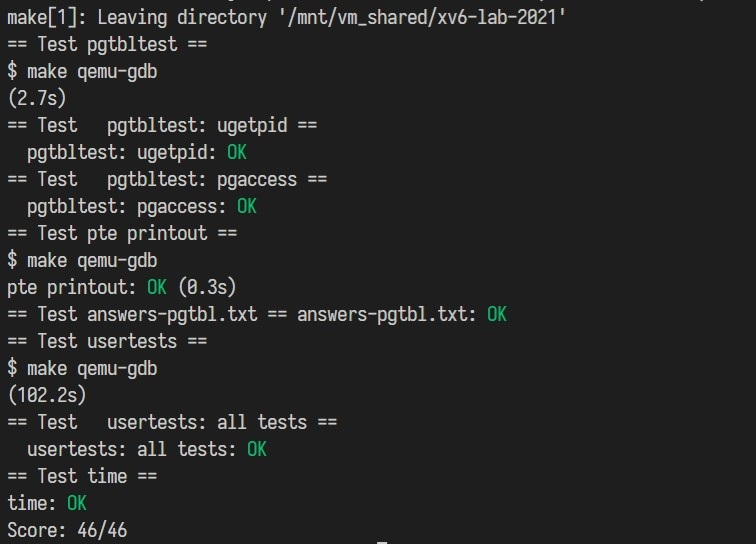
\includegraphics[width=0.8\textwidth]{pgtbl_grade.jpg}
  \caption{ Lab Page tables 的测评结果}
\end{figure}
可见测试全部通过,得分为满分。


\section{小结:RISC-V 的页表机制}

通过上面的几个实验,我们能够大致了解 RISC-V 的 MMU 硬件提供的分页机制与操作系统配合的全过程。但是,上面的实验里没有详细地总结 RISC-V 硬件的的分页机制,这里我们将参考 RISC-V 的手册 \textit{The RISC-V Instruction Set Manual: Volume II: Privileged Architecture} \footnote{\url{https://riscv.org/wp-content/uploads/2017/05/riscv-privileged-v1.10.pdf}} 对 RISC-V 中最常用的 Sv-39 ( Page-Based 39-bit Virtual-Memory System ) 分页机制进行一个小结。

\begin{figure}[H]
  \centering
  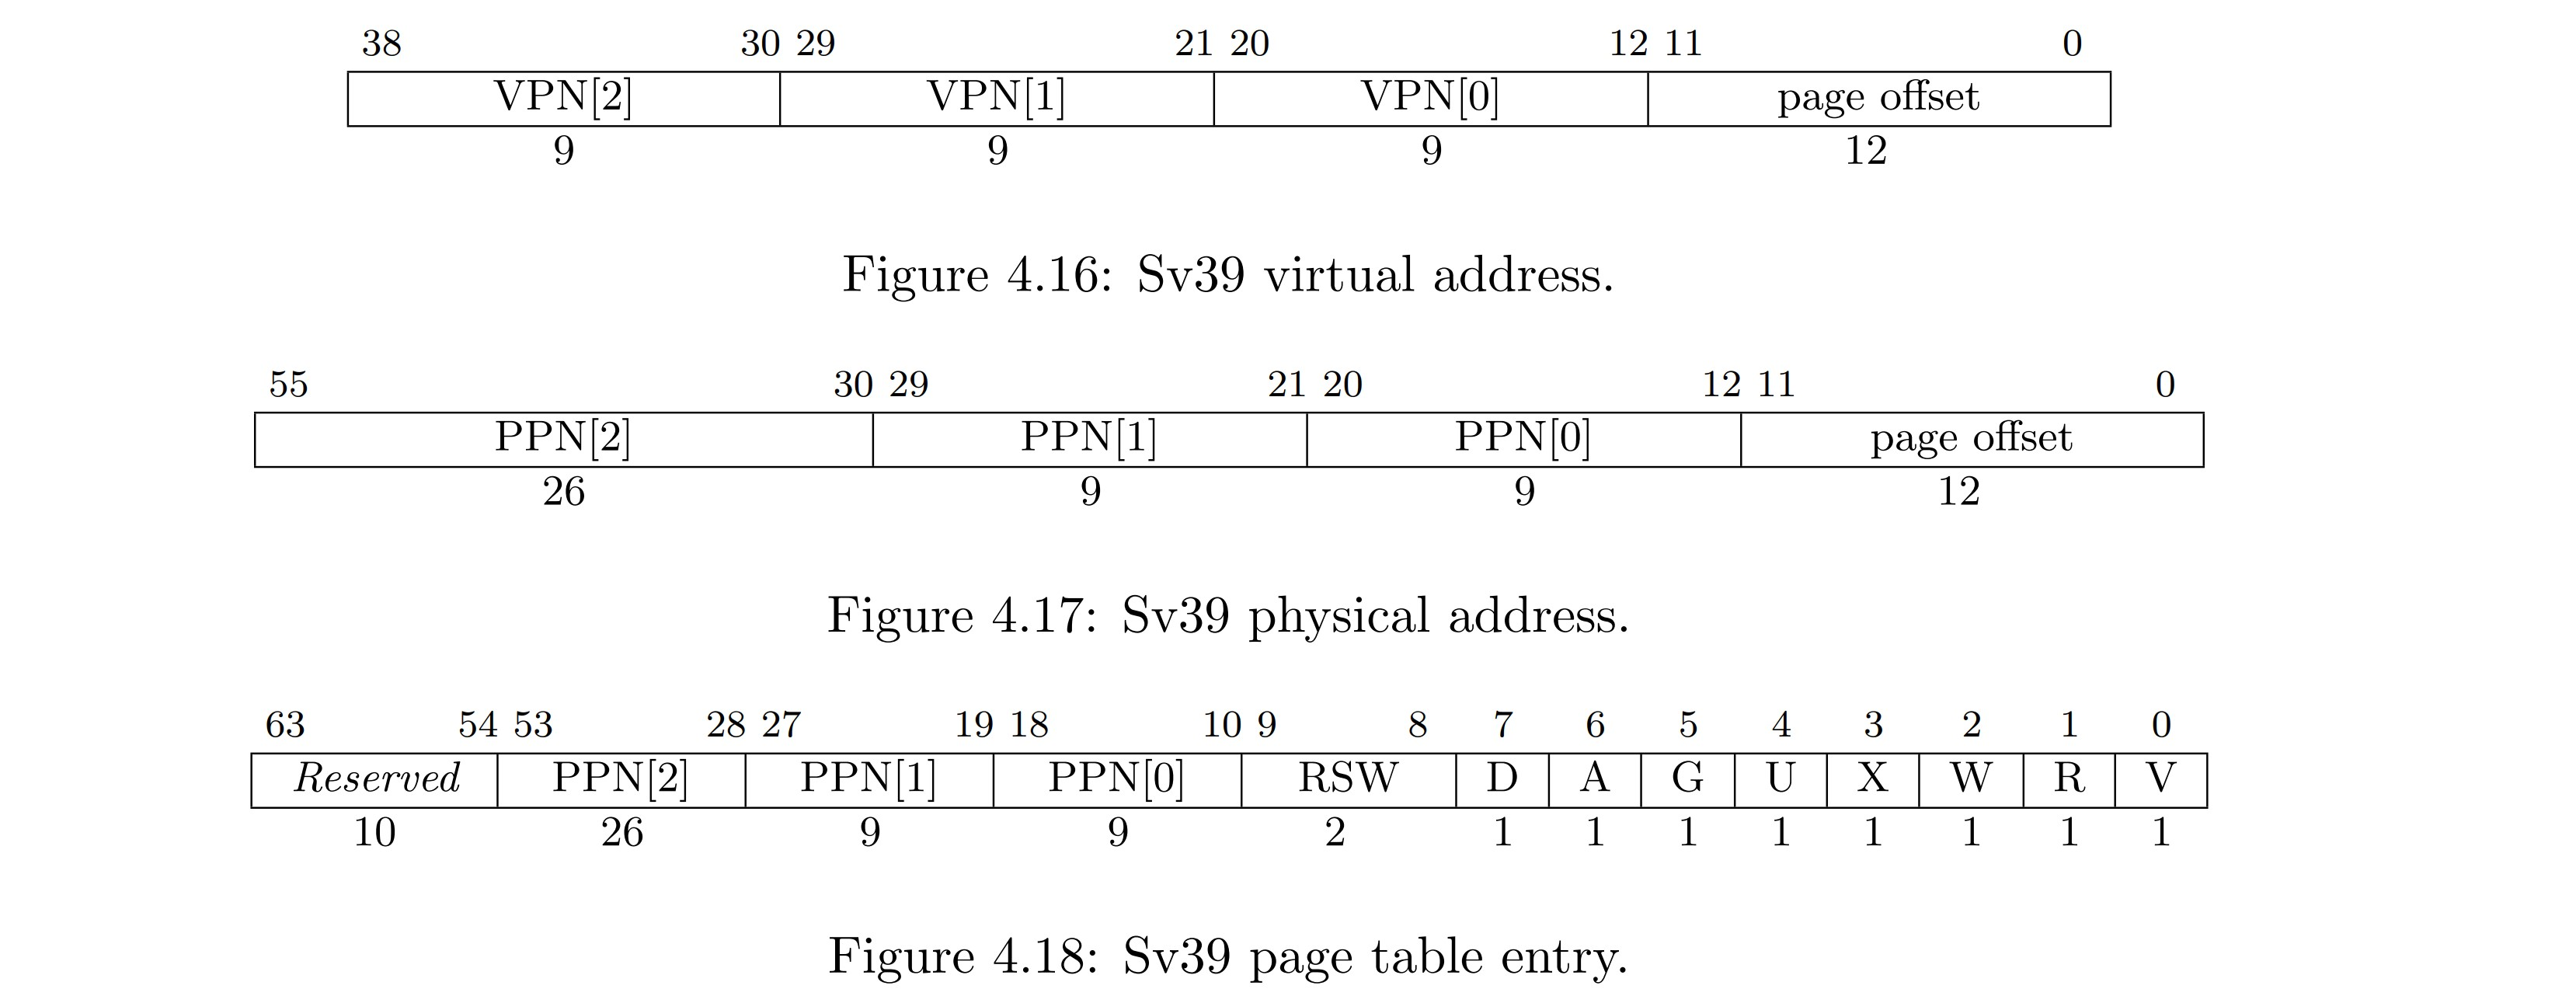
\includegraphics[width=1.0\textwidth]{pgtbl_sv39.jpg}
  \caption{ RISC-V 手册中关于 Sv-39 的图解(手册 p.63 ) }
\end{figure}

上图即RISC-V 手册中关于 Sv-39 的总结。参考对应上图中的 Figure 4.16 ,顾名思义, Sv-39 的支持 39 位的虚拟地址,即 64 位的低 39 位是有效的,高位均为第 38 位的值;其一个页面大小为 4KB (必须边界对齐,即页面起始地址的低 12 位必须均为 0 ) ,故整个 39 位的地址的 0 到 11 位是页内偏移,在地址变换时不发生变化。

除去页内偏移外,剩余高的 27 位被等分为了 3 段,每段各 9 位;每一段对应各级页表,故 Sv-39 是一个三级页表的系统 (比 x86 架构的 32 位二级页表要多一级),而每段的 9 位的 VPN (虚存页面编号)对应该级页表中的项,即每一个页表中有 $2^9 = 512$ 项,这与页面大小是匹配的,因为每个页表项为 64 位 (见上图中的 Figure 4.18 ),即 8 Byte ,故整个页表的大小恰好为 4KB ,即一页的大小。

在 Sv-39 中,物理地址的格式对应上图中的 Figure 4.17 ,与虚拟地址类似,页面大小为 4KB 且边界对齐;除了低位的 12 位页内偏移外,高位为物理的页号(共 44 位物理页号)。对于页表项,高位的未使用的 54 到 63 位始终置 0 ,而后是 44 位物理页号,而后的第 9 位和第 8 位是供操作系统自定义使用的,而后的第 0 到第 7 位是该页面的状态位、权限设置和属性等。具体的 0 到 7 位的含义如下:
\begin{itemize}
    \item 第 7 位, Dirty bit ,对应的页面被写入后会被硬件置为 1 ,可被操作系统置为 0
    \item 第 6 位, Access bit ,对应的页面被访问后会被硬件置为 1 ,可被操作系统置为 0
    \item 第 5 位, Global bit ,其为 1 表示该页表项的映射对所有的内存空间均有效
    \item 第 4 位到第 1 位, User/Read/Write/eXecute bit,用于控制页面的权限,由操作系统设置
    \item 第 0 位,Valid bit,页表项的有效位
\end{itemize}

在使用 Sv-39 分页机制进行内存地址转换时,根页表的物理页面号 PPN 会被存储在 SATP 寄存器的 PPN 号的区间内,且 SATP 寄存器的 MODE 段(分页模式)和 ASID 段(地址空间)都被设为进程对应的值。某个指令访问某个虚拟地址时,处理器会:
\begin{enumerate}
    \item 读取 SATP 寄存器的 PPN 对应的页表根页面,
    \item 然后依次沿着各级 VPN (虚存页面编号)找到虚拟地址对应的页表项,
    \item 检查权限无误后,根据指令的操作设置该页表项的 Dirty/Access 位,
    \item 并且用该页表项的 PPN 与指令的页内偏移拼接,得到物理地址,
    \item 然后执行指令的操作。
\end{enumerate}

更加形象化的表述如下图所示:
\begin{figure}[H]
  \centering
  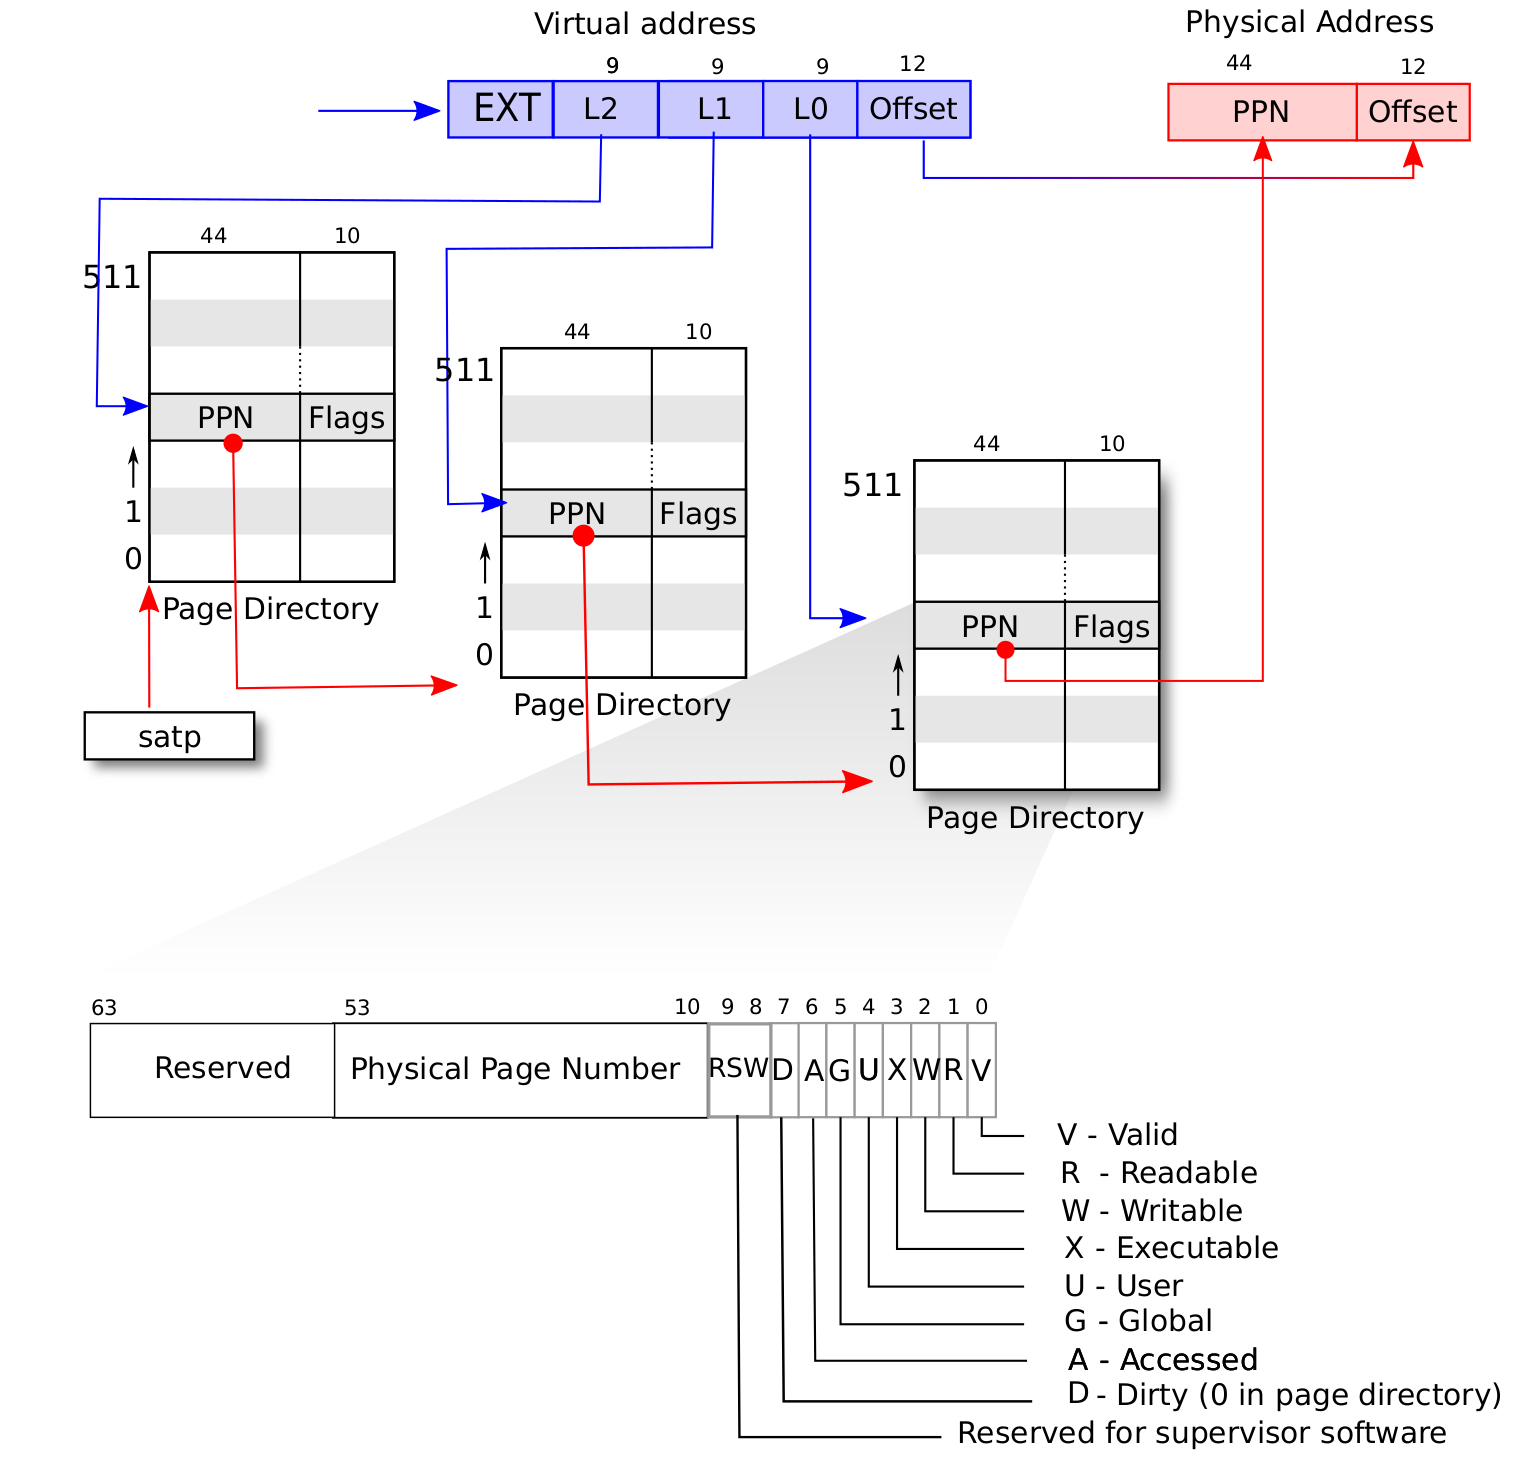
\includegraphics[width=0.8\textwidth]{pgtbl_sv39-full.png}
  \caption{ Sv-39 地址转换的过程(来源于 MIT 6.828 课程) }
\end{figure}

我们的 xv6 操作系统在 RISC-V 平台上借助的硬件分页机制就是 Sv39 ,若要将 xv6 移植到其它硬件平台上(如 s390x, 龙芯等),则需要根据其硬件提供的分页机制重写有关分页机制初始化和页表操作的代码。

\begin{proposition}[关于大页 ( Huge Page )]
    由于现代的应用软件占据的内存逐渐增大,主流的计算机硬件(如 x64 平台)逐渐开始支持较大的页面(如 x64 支持的 2MiB 的大页)。RISC-V 作为先进的架构,同样也在 Sv39 分页模式中支持大页,而且其支持两种不同尺寸的大页:大小为 2MiB 的页被称为 \textit{megapages} ,而大小为 1GiB 的页被称为 \textit{gigapages} 。这两类大页都需要进行边界对齐(例如一个 \textit{gigapage} 开始的物理地址和虚拟地址的低 30 位必须均为 0)。大页的机制提供了更好的访存性能,且可以很好地融入目前的 Sv39 分页模式中。
\end{proposition}

得益于硬件制造技术的进步, Sv-39 提供的 39 位虚拟地址空间和 56 位物理地址空间逐渐无法适应一些新的硬件:越来越多的计算机已经配置了超过 512 GiB 的物理内存(比如笔者的工作站,安装的物理内存为 1.5 TiB )。 RISC-V 除了提供 Sv-39 的分页机制外,同样也提供了基于四级页表的 Sv-48 分页机制。该机制支持 48 位的虚拟地址,且提供了 4KB , 2MB , 1GB和 512GB 四种可选的页面大小,预计足够未来数年的硬件使用。
\chapter{Lab Traps:中断实验}
\begin{introduction}
    \item 学习 RISC-V 汇编
    \item 实现 Backtrace 
    \item 实现定时器系统调用
    \item RISC-V 的中断机制
\end{introduction}

除了上一章实验的页表机制外,中断机制也是组成操作系统不可或缺的部分。本章的实验主要集中于 xv6 的中断机制,通过改进 xv6 的中断机制来学习并应用关于中断的一些概念。

\section{学习 RISC-V 汇编}

由于本次实验及之后的实验中,会涉及到机器指令级别的操作和调试,故而了解一些关于 RISC-V 汇编的知识将有助于实验的进行。这个实验几乎不需要编写代码,主要内容是观察一些汇编代码和它们的行为。

我们首先需要使用\lstinline{make} 将 \lstinline{user/call.c} 源文件编译为对应的目标代码,在这个过程中, xv6 的 Makefile 会自动生成反汇编后的代码。编译完成后,打开新生成的 \lstinline{user/call.asm},回答 xv6 实验手册中提出的问题。

\begin{lstlisting}
user/_call:     file format elf64-littleriscv


Disassembly of section .text:

0000000000000000 <g>:
#include "kernel/param.h"
#include "kernel/types.h"
#include "kernel/stat.h"
#include "user/user.h"

int g(int x) {
   0:	1141                	addi	sp,sp,-16
   2:	e422                	sd	s0,8(sp)
   4:	0800                	addi	s0,sp,16
  return x+3;
}
   6:	250d                	addiw	a0,a0,3
   8:	6422                	ld	s0,8(sp)
   a:	0141                	addi	sp,sp,16
   c:	8082                	ret

000000000000000e <f>:

int f(int x) {
   e:	1141                	addi	sp,sp,-16
  10:	e422                	sd	s0,8(sp)
  12:	0800                	addi	s0,sp,16
  return g(x);
}
  14:	250d                	addiw	a0,a0,3
  16:	6422                	ld	s0,8(sp)
  18:	0141                	addi	sp,sp,16
  1a:	8082                	ret

000000000000001c <main>:

void main(void) {
  1c:	1141                	addi	sp,sp,-16
  1e:	e406                	sd	ra,8(sp)
  20:	e022                	sd	s0,0(sp)
  22:	0800                	addi	s0,sp,16
  printf("%d %d\n", f(8)+1, 13);
  24:	4635                	li	a2,13
  26:	45b1                	li	a1,12
  28:	00000517          	auipc	a0,0x0
  2c:	7c050513          	addi	a0,a0,1984 # 7e8 <malloc+0xea>
  30:	00000097          	auipc	ra,0x0
  34:	610080e7          	jalr	1552(ra) # 640 <printf>
  exit(0);
  38:	4501                	li	a0,0
  3a:	00000097          	auipc	ra,0x0
  3e:	27e080e7          	jalr	638(ra) # 2b8 <exit>
......
\end{lstlisting}

\begin{exercise}
    Which registers contain arguments to functions? For example, which register holds 13 in main's call to \lstinline{printf}?
\end{exercise}

\begin{solution}
根据 RISC-V 的 ABI 手册 \footnote{\url{https://pdos.csail.mit.edu/6.828/2021/readings/riscv-calling.pdf}} ,寄存器 a0 到 a7 (即寄存器 x10 到 x17 )用于存放函数调用的参数。

对于上面 \lstinline{user/call.c} 中的\lstinline{printf} ,我们查阅其汇编代码,关注如下代码段:
\begin{lstlisting}
......
  printf("%d %d\n", f(8)+1, 13);
  24:	4635                	li	a2,13
  26:	45b1                	li	a1,12
  28:	00000517          	auipc	a0,0x0
  2c:	7c050513          	addi	a0,a0,1984 # 7e8 <malloc+0xea>
  30:	00000097          	auipc	ra,0x0
  34:	610080e7          	jalr	1552(ra) # 640 <printf>
......
\end{lstlisting}

不难发现,在 \lstinline{jalr 1552(ra)} 跳转至 \lstinline{printf} 执行前,一条指令 \lstinline{li	a2,13} 将参数 13 存放在寄存器 a2 中。
\end{solution}

\begin{proposition}[寄存器的名字] 
我们在查看 RISC-V 的文档时,时常会发现两种寄存器的名字:一种以 x 开头,后面直接跟寄存器的编号;一种则表示寄存器的通常用途,如 ra 、 sp 、 tp 、 a0 等。这两种用法都十分常见,可能后者使用得要略多一点。对于不熟悉操作系统的同学来说,如 ra 、 sp 、 a0 等寄存器的名字会有些费解,其实这些名字都是英文短语的缩写,例如 ra 是 return address (返回地址)的缩写, sp 是 stack pointer (栈指针)的缩写,而 a0 等名称中的 a 则是 argument (参数)的缩写。
\end{proposition}

\begin{exercise}
    Where is the call to function \lstinline{f} in the assembly code for main? Where is the call to \lstinline{g}? (Hint: the compiler may inline functions.)
\end{exercise}

\begin{solution}

由于在 \lstinline{user/call.c} 中, \lstinline{f} 被 \lstinline[language=C]{printf("%d %d\n", f(8)+1, 13)} 调用,故而我们先查看汇编代码中与 \lstinline{printf} 相关的代码:
\begin{lstlisting}
......
  printf("%d %d\n", f(8)+1, 13);
  24:	4635                	li	a2,13
  26:	45b1                	li	a1,12
  28:	00000517          	auipc	a0,0x0
  2c:	7c050513          	addi	a0,a0,1984 # 7e8 <malloc+0xea>
  30:	00000097          	auipc	ra,0x0
  34:	610080e7          	jalr	1552(ra) # 640 <printf>
......
\end{lstlisting}

在跳转至 \lstinline{printf} 执行前,一条指令 \lstinline{li	a1,12} 直接将立即数 12 存放在寄存器 a1 中,而该立即数恰好是调用 \lstinline{f(8)+1} 结果,可见编译器优化直接通过常量优化的方式将常量值计算出来填入了 \lstinline{printf} 的参数中,而没有真正执行 \lstinline{f} 。

对于 \lstinline{g} 的调用,关注如下代码段:
\begin{lstlisting}
......
000000000000000e <f>:

int f(int x) {
   e:	1141                	addi	sp,sp,-16
  10:	e422                	sd	s0,8(sp)
  12:	0800                	addi	s0,sp,16
  return g(x);
}
  14:	250d                	addiw	a0,a0,3
  16:	6422                	ld	s0,8(sp)
  18:	0141                	addi	sp,sp,16
  1a:	8082                	ret
......
\end{lstlisting}

在 \lstinline{f} 中调用了 \lstinline{g} ,但是编译器对于这种较短的函数,直接将函数内联至 \lstinline{f} 中,以减少压栈和跳转的开销。实际上执行 \lstinline{g} 的代码是 \lstinline{14:	250d addiw a0,a0,3} 。
\end{solution}

\begin{theorem}[关于编译器优化]
    现代编译器优化的能力已经达到了“令人发指”的地步,以至于专业的汇编语言程序员都很难写出和打开了 \lstinline{-O2} 优化选项一样高效的汇编代码。常见的编译优化手段,如复写传播,删除死代码, 强度削弱,归纳变量删除,代码外提等,配合一些启发式的优化手段,可以大大提高高级语言书写的程序在实际机器上运行的效率。但这些强大的优化手段也带来了调试上的困难,一个经常遇到的情况是,当在使用 gdb 等调试器调试代码时,一些变量会给出形如 \lstinline{<value optimized out>} 的结果,从而妨碍调试的进行。为了解决这种问题,一般有几种方法: 1)在 Makefile 里指定编译优化选项为 \lstinline{-O0} 或 \lstinline{-Og} ; 2)使用特定的编译选项如 \lstinline{-fno-inline} ;3)对特定的函数添加 attribute ,如 \lstinline{int func(int arg) __attribute__((noinline))}。
\end{theorem}

\begin{exercise}
    At what address is the function printf located?
\end{exercise}

\begin{solution}
关注 \lstinline{user/call.asm} 中的如下代码:
\begin{lstlisting}
......
0000000000000640 <printf>:

void
printf(const char *fmt, ...)
{
 640:	711d                	addi	sp,sp,-96
......
\end{lstlisting}

故其地址为 0x640 。
\end{solution}

\begin{exercise}
    What value is in the register ra just after the jalr to printf in main?
\end{exercise}

\begin{solution}
关注 \lstinline{user/call.asm} 中的如下代码:
\begin{lstlisting}
......
34:	610080e7          	jalr	1552(ra) # 640 <printf>
......
\end{lstlisting}

故 ra 寄存器中存储的地址为 0x38 。
\end{solution}

\begin{exercise}
Run the following code.
\begin{lstlisting}
	unsigned int i = 0x00646c72;
	printf("H%x Wo%s", 57616, &i);
\end{lstlisting}
What is the output? Here's an ASCII table \footnote{http://web.cs.mun.ca/~michael/c/ascii-table.html} that maps bytes to characters.

The output depends on that fact that the RISC-V is little-endian. If the RISC-V were instead big-endian what would you set i to in order to yield the same output? Would you need to change 57616 to a different value?
\end{exercise}

\begin{solution}
将上述代码加入到 \lstinline{user/call.c} 中,编译运行,得到的输出为: \lstinline{HE110 World} 。

57616 的十六进制表示是 E110, 且 0x72, 0x6c, 0x64 转为 ASCII 为 r, l和 d。 如果是大端序的话,将 i 改为 0x726c6400 即可,无需改变 57616。
\end{solution}

\begin{exercise}
    In the following code, what is going to be printed after \lstinline{'y='}? (note: the answer is not a specific value.) Why does this happen?
\begin{lstlisting}
    printf("x=%d y=%d", 3);
\end{lstlisting}
\end{exercise}

\begin{solution}
将上述代码加入到 \lstinline{user/call.c} 中,编译运行,得到的输出为: \lstinline{x=3 y=1} 。产生这样输出的原因在于恰好后一个 \lstinline{%d} 访问的地址中的数据的十进制表示为 1 。
\end{solution}

\section{实现 Backtrace }

因为 gdb 等调试工具很难进行内核态的调试,为了便于调试内核,在内核中实现 backtrace 函数是大有裨益的。我们需要在 \lstinline{kernel/printf.c} 实现 \lstinline{backtrace()} ,并且在 \lstinline{sys_sleep} 调用中插入一个 \lstinline{backtrace()} 函数,用以打印当时的栈。为了检验实现的正确性, xv6 实验提供了 \lstinline{bttest} 程序,运行时打印的内容应当如下:
\begin{lstlisting}
backtrace:
0x0000000080002cda
0x0000000080002bb6
0x0000000080002898
\end{lstlisting}

看到上述内容,退出 qemu 后,运行 \lstinline{riscv64-unknown-elf-addr2line -e kernel/kernel} ,将 \lstinline{bttest} 程序的输出粘贴进去,按下 Ctrl + D ,即可得到如下的输出:
\begin{lstlisting}
    $ addr2line -e kernel/kernel
    0x0000000080002de2
    0x0000000080002f4a
    0x0000000080002bfc
    Ctrl-D
    kernel/sysproc.c:74
    kernel/syscall.c:224
    kernel/trap.c:85
\end{lstlisting}

为了实现 \lstinline{backtrace()} 函数,我们需要阅读 RISC-V ABI 文档和一些已经编译好的汇编代码。再次回顾上面的 \lstinline{user/call.asm} 中一个函数的调用过程:
\begin{lstlisting}
......
void main(void) {
  1c:	1141                	addi	sp,sp,-16
  1e:	e406                	sd	ra,8(sp)
  20:	e022                	sd	s0,0(sp)
  22:	0800                	addi	s0,sp,16
  printf("%d %d\n", f(8)+1, 13);
  24:	4635                	li	a2,13
  26:	45b1                	li	a1,12
  28:	00000517          	auipc	a0,0x0
  2c:	7c050513          	addi	a0,a0,1984 # 7e8 <malloc+0xea>
  30:	00000097          	auipc	ra,0x0
  34:	610080e7          	jalr	1552(ra) # 640 <printf>
......
\end{lstlisting}

进入 \lstinline{main} 函数前,由于栈是从高地址向低地址扩展,所以该程序首先执行 \lstinline{addi sp,sp,-16} 将栈向下生长,然后执行两条指令将返回地址 ra 和 栈的基地址 s0 存储到栈中。调用其它函数的最开始的几个指令也如出一辙,如 \lstinline{printf} 函数:
\begin{lstlisting}
......
0000000000000640 <printf>:

void
printf(const char *fmt, ...)
{
 640:	711d                	addi	sp,sp,-96
 642:	ec06                	sd	ra,24(sp)
 644:	e822                	sd	s0,16(sp)
 646:	1000                	addi	s0,sp,32
 648:	e40c                	sd	a1,8(s0)
 64a:	e810                	sd	a2,16(s0)
 64c:	ec14                	sd	a3,24(s0)
 64e:	f018                	sd	a4,32(s0)
 650:	f41c                	sd	a5,40(s0)
 652:	03043823          	sd	a6,48(s0)
 656:	03143c23          	sd	a7,56(s0)
......
\end{lstlisting}

只是顺带多保存了一些参数到栈中供 \lstinline{printf} 函数使用,其 sp 、 ra 、 s0 的相对位置关系仍然和文档中一致。

我们的 \lstinline{backtrace()} 函数只需打印每次保存的 ra 即可,然后根据 s0 的值寻找上一个栈帧,然后继续打印保存的 ra ,如此往复直到到达栈底。根据 xv6 实验指导的提醒,我们首先在 \lstinline{kernel/riscv.h} 中加入以下内联汇编函数用于读取当前的 s0 寄存器:
\begin{lstlisting}[language=C]
static inline uint64
r_fp()
{
  uint64 x;
  asm volatile("mv %0, s0" : "=r" (x) );
  return x;
}
\end{lstlisting}

然后利用上面的思想,在 \lstinline{kernel/printf.c} 实现 \lstinline{backtrace()}, 笔者的实现如下:
\begin{lstlisting}[language=C]
void
backtrace(void)
{
  printf("backtrace:\n");
  for (uint64 *fp = (uint64 *)r_fp(); (uint64)fp < PGROUNDUP((uint64)fp); fp = (uint64 *)(*(fp-2)))
  {
    printf("%p\n",*(fp-1));
  }
}
\end{lstlisting}

其中用到了一些关于指针算数的小技巧。实现完成后,在 \lstinline{sys_sleep} 调用中插入一个 \lstinline{backtrace()} 函数:
\begin{lstlisting}[language=C]
uint64
sys_sleep(void)
{
  int n;
  uint ticks0;
  backtrace();
......
\end{lstlisting}

然后编译运行 xv6 ,然后执行 \lstinline{bttest} , 将其输出粘贴到 \lstinline{addr2line -e kernel/kernel} 中,结果如下图所示:
\begin{figure}[H]
  \centering
  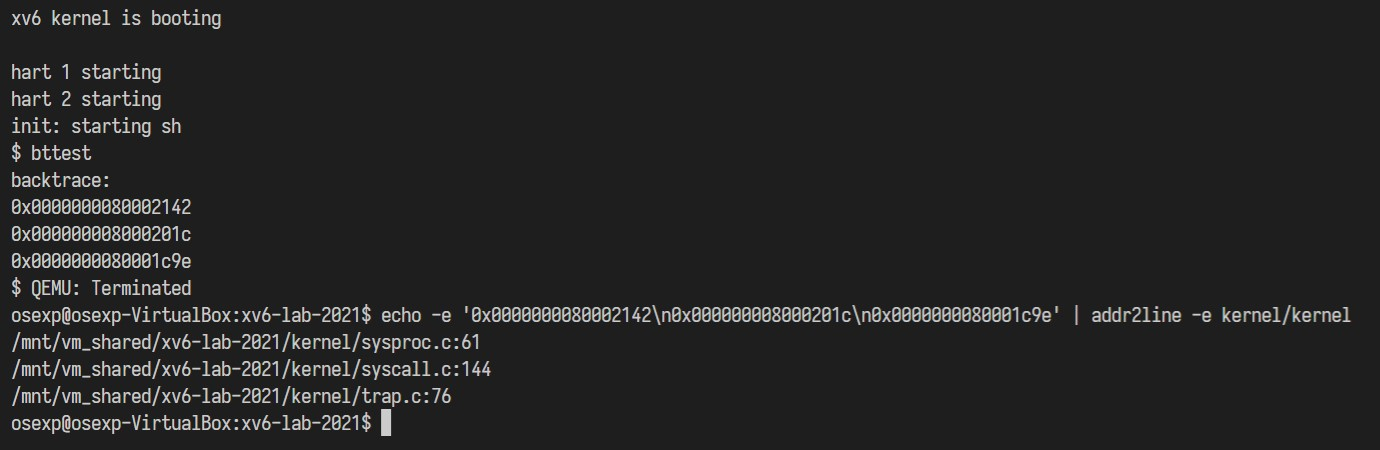
\includegraphics[width=0.8\textwidth]{traps_bttest.jpg}
  \caption{ 验证 \lstinline{backtrace()} 正确性的结果 }
\end{figure}
可见与预期相同,说明实现正确。

\section{实现定时器系统调用}

为了让一个进程能够在消耗一定的 CPU 时间后被告知,我们需要实现 \lstinline{sigalarm(n, fn)} 系统调用。用户程序执行 \lstinline{sigalarm(n, fn)} 系统调用后,将会在其每消耗 n 个 tick 的 CPU 时间后被中断并且运行其给定的函数 fn 。这个系统调用对于不希望占用过多 CPU 时间,或希望进行周期性操作的程序来说是及其有用的。此外,实现 \lstinline{sigalarm(n, fn)} 系统调用有利于我们学会如何构建用户态的中断和中断处理程序,这样就可以使用类似的方法使用户态程序可以处理缺页等常见的异常。

如果我们的实现正确,则运行 \lstinline{usertests} 和 \lstinline{alarmtest} 均会通过。

正确实现 \lstinline{sigalarm(n, fn)} 系统调用面临以下几个问题:
\begin{enumerate}
    \item 如何保存每个进程的 \lstinline{sigalarm} 参数;
    \item 如何并更新每个已经消耗的 tick 数;
    \item 如何在已经消耗的 tick 数符合要求时使进程调用中断处理过程 fn ;
    \item 中断处理过程 fn 执行完毕后如何返回。
\end{enumerate}

在解决这些问题前,我们先照例在 \lstinline{user/user.h} 加入两个系统调用的入口,分别用于设置定时器和从定时器中断处理过程中返回:
\begin{lstlisting}[language=C]
    int sigalarm(int ticks, void (*handler)());
    int sigreturn(void);
\end{lstlisting}

首先解决第一个问题,联想到 Lab System calls 中 trace 的实现,我们需要在每个进程的控制块的数据结构中加入存储 \lstinline{sigalarm(n, fn)} 中参数的项,即在 \lstinline{kernel/proc.h} 的 \lstinline{struct proc}中加入如下的项:
\begin{lstlisting}[language=C]
    int alarminterval;           // sys_sigalarm() alarm interval in ticks
    int alarmticks;              // sys_sigalarm() alarm interval in ticks
    void (*alarmhandler)();      // sys_sigalarm() pointer to the alarm handler
    int sigreturned;
\end{lstlisting}

然后在 \lstinline{kernel/proc.c} 的 \lstinline{allocproc(void)} 中对这些变量进行初始化:
\begin{lstlisting}[language=C]
static struct proc*
allocproc(void)
{
......
  // Initialize alarmticks
  p->alarmticks = 0;
  p->alarminterval = 0;
  p->sigreturned = 1;
  return p;
}
\end{lstlisting}

初始化后,在调用 \lstinline{sigalarm(n, fn)} 系统调用时,执行的 \lstinline{kernel/sysproc.c} 中的 \lstinline{sys_sigalarm()} 需根据传入的参数设置 \lstinline{struct proc} 的对应项:
\begin{lstlisting}[language=C]
uint64
sys_sigalarm(void)
{
  int ticks;
  uint64 handler;
  struct proc *p = myproc();
  if(argint(0, &ticks) < 0 || argaddr(1, &handler) < 0)
    return -1;
  p->alarminterval = ticks;
  p->alarmhandler = (void (*)())handler;
  p->alarmticks = 0;
  return 0;
}
\end{lstlisting}

可以在 \lstinline{sys_sigalarm(void)} 加入打印语句用于 debug ,确认参数传入无误后可以着手解决第二个问题。

如何并更新每个已经消耗的 tick 数,我们需要修改定时器中断发生时的行为,为每个有 \lstinline{sigalarm} 的进程更新其已经消耗的 tick 数。打开 \lstinline{kernel/trap.c} ,在 \lstinline{usertrap()} 中的判断是否为定时器中断的 if 语句块中加入对应的实现:

\begin{lstlisting}[language=C]
......
  if(which_dev == 2)
  {
    p->alarmticks += 1;
......
\end{lstlisting}

然后顺手解决第三个问题,判断该进程已经使用的 tick 数是否已经足以触发 alarm :
\begin{lstlisting}[language=C]
......
if(which_dev == 2)
{
  p->alarmticks += 1;
  if ((p->alarmticks >= p->alarminterval) && (p->alarminterval > 0))
  {
    p->alarmticks = 0;
......
  }
  yield();
}
......
\end{lstlisting}

若 ticks 达到了预先设定的值,则将计数器清零,并使得用户进程跳至预设的处理过程 fn 处执行。首先我们需要在 \lstinline{struct proc} 增设 \lstinline{alarmtrapframe} 用于备份进程当前的上下文:
\begin{lstlisting}[language=C]
......
  int alarminterval;           // sys_sigalarm() alarm interval in ticks
  int alarmticks;              // sys_sigalarm() alarm interval in ticks
  void (*alarmhandler)();      // sys_sigalarm() pointer to the alarm handler
  struct trapframe alarmtrapframe; // for saving registers
  int sigreturned;
......
\end{lstlisting}

然后,在 \lstinline{usertrap()} 中备份当前的上下文,并将用户态的程序计数器设置到 fn 处,然后完成该定时器调用,返回到用户态:
\begin{lstlisting}[language=C]
......
if(which_dev == 2)
{
  p->alarmticks += 1;
  if ((p->alarmticks >= p->alarminterval) && (p->alarminterval > 0))
  {
    p->alarmticks = 0;
    if (p->sigreturned == 1)
    {
      p->alarmtrapframe = *(p->trapframe);
      p->trapframe->epc = (uint64)p->alarmhandler;
      p->sigreturned = 0;
      usertrapret();
    }
  }
  yield();
}
......
\end{lstlisting}

这样整个触发 \lstinline{sigalarm} 的过程便成功完成了。此时还剩最后一个问题没有解决:当传入的 fn 执行完毕后,如何返回到进程正常的执行过程中。由于之前我们保存了进程执行的上下文,故而在 fn 调用 \lstinline{sigreturn()} 时,我们需要在内核态对应的 \lstinline{sys_sigreturn()} 中将备份的上下文恢复,然后返回用户态,该实现依然放在 \lstinline{kernel/sysproc.c} 中:
\begin{lstlisting}[language=C]
......
uint64
sys_sigreturn(void)
{
  struct proc *p = myproc();
  p->sigreturned = 1;
  *(p->trapframe) = p->alarmtrapframe;
  usertrapret();
  return 0;
}
......
\end{lstlisting}

至此,整个 alarm 机制便实现完成了。编译并启动 xv6 后,在 shell 中运行 \lstinline{alarmtest} ,即可看到预期的输出,如下图所示:
\begin{figure}[H]
  \centering
  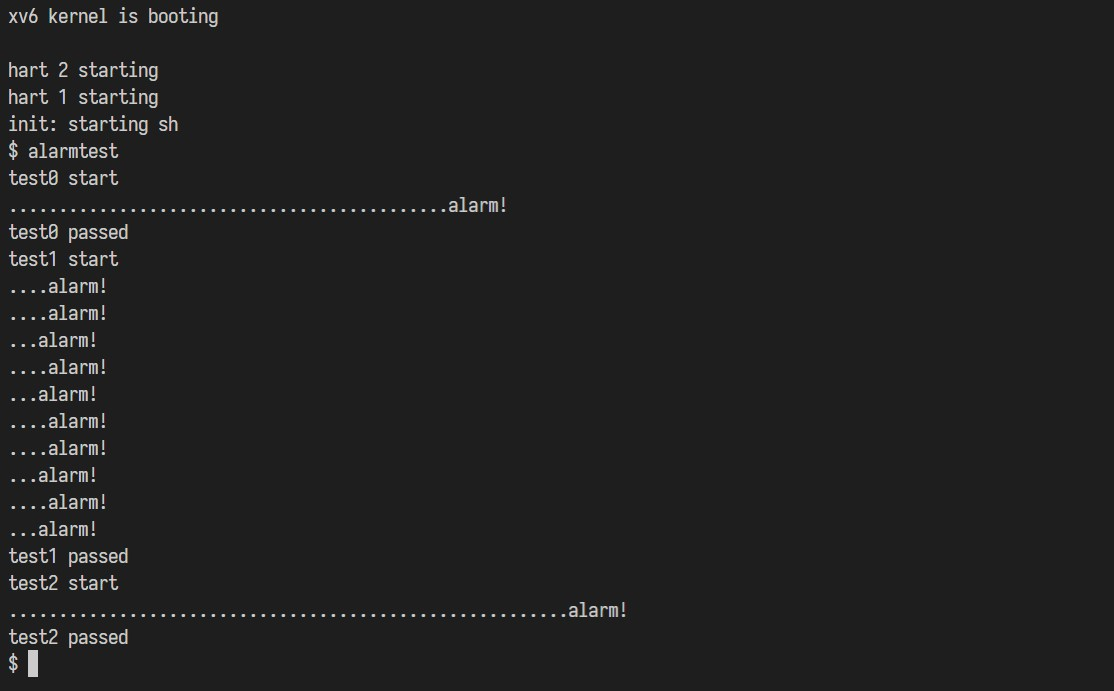
\includegraphics[width=0.8\textwidth]{traps_alarmtest.jpg}
  \caption{ 验证 alarm 机制的正确性 }
\end{figure}

\paragraph*{实验结果} 在完成 Lab Traps 中的所有实验后,根据 MIT 6.S081 的传统,需要在实验目录下创建一个名为 \lstinline{time.txt} 文本文件,其中只包含一行,为完成该实验的小时数。然后在终端中执行 \lstinline{make grade} ,即可对整个实验进行自动评分,笔者的结果如下:
\begin{figure}[H]
  \centering
  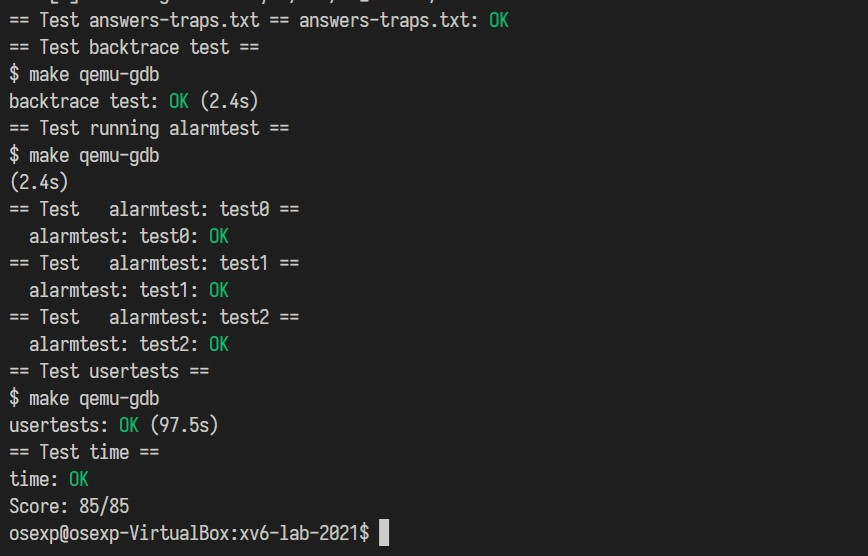
\includegraphics[width=0.8\textwidth]{traps_grade.jpg}
  \caption{ Lab Traps 的测评结果}
\end{figure}
可见测试全部通过,得分为满分。

\section{小结:RISC-V 的中断机制}

上面的实验中,我们首先了解了 RISC-V 的汇编及其 ABI 的一些内容,从而结合定时器中断来实现 alarm 的机制。实验中没有详细地讲解整个 RISC-V 的中断机制,故而笔者在这里对 xv6 涉及到的 RISC-V 的中断机制进行一个小结,这里我们主要参考 RISC-V 的手册 \textit{The RISC-V Instruction Set Manual: Volume II: Privileged Architecture} \footnote{\url{https://riscv.org/wp-content/uploads/2017/05/riscv-privileged-v1.10.pdf}} 。

我们首先考察 xv6 在启动时执行的一些初始化代码,在 \lstinline{kernel/start.c} 中,有如下的代码段:
\begin{lstlisting}[language=C]
......
  // set the machine-mode trap handler.
  w_mtvec((uint64)timervec);

  // enable machine-mode interrupts.
  w_mstatus(r_mstatus() | MSTATUS_MIE);
......
\end{lstlisting}

在 \lstinline{kernel/main.c} 中,有如下的代码段:
\begin{lstlisting}[language=C]
......
    trapinit();      // trap vectors
    trapinithart();  // install kernel trap vector
    plicinit();      // set up interrupt controller
    plicinithart();  // ask PLIC for device interrupts
......
\end{lstlisting}


这些初始化用的函数与中断相关。从这些初始化代码中不难发现, RiSC-V 管理中断的方式主要有几类:(裸机启动时的)定时器中断、来自内核的中断和通过 PLIC 管理的设备中断。

以来自内核态的中断为例展开介绍。对于内核态的中断,我们初始化时已经将对应的中断处理程序 \lstinline{kernel/kernelvec.S} 的地址放在了 STVEC 寄存器( Supervisor Trap Vector Base Address Register )中,见 \lstinline{kernel/trap.c} :
\begin{lstlisting}[language=C]
// set up to take exceptions and traps while in the kernel.
void
trapinithart(void)
{
  w_stvec((uint64)kernelvec);
}
\end{lstlisting}

这样,当内核态的中断发生时, CPU 会自动从 STVEC 寄存器指向的指令开始执行,即执行 \lstinline{kernel/kernelvec.S} 中的代码,具体工作为在内核栈中保存上下文,并调用 \lstinline{kernel/trap.c} 中的 \lstinline{kerneltrap()} ,调用完成后恢复栈中保存的上下文,继续运行内核原来正在进行的代码。

在 \lstinline{kerneltrap()} 中,涉及到一些描述中断状态的寄存器,其中较为重要的有 SEPC (  Supervisor Exception Program Counter 用于记录中断时的 PC )、 SSTATUS ( Supervisor Status Register 用于记录中断时的状态 )和 SCAUSE ( Supervisor Cause Register 用于记录中断的原因 )。 \lstinline{kerneltrap()} 会检查这些寄存器,从而判断中断是否合法。

类似的,对于由 \lstinline{ecall} 导致的中断,CPU 同样会自动从 STVEC 寄存器指向的指令开始执行,只是此时由于进程运行在用户态,故而 STVEC 寄存器在之前就已经被设为了 \lstinline{trampoline} 过程对应的首地址(在 \lstinline{kernel/trap.c} 中):
\begin{lstlisting}[language=C]
void
usertrapret(void)
{
......
  // send syscalls, interrupts, and exceptions to trampoline.S
  w_stvec(TRAMPOLINE + (uservec - trampoline));
......
\end{lstlisting}

在 \lstinline{kernel/trampoline.S} 调用 \lstinline{usertrap()} 后,处理器已经进入内核态(S态),此时 STVEC 寄存器的指向的地址又被设为了 \lstinline{kernel/kernelvec.S} 的地址:
\begin{lstlisting}[language=C]
void
usertrap(void)
{
......
  // send interrupts and exceptions to kerneltrap(),
  // since we're now in the kernel.
  w_stvec((uint64)kernelvec);
......
\end{lstlisting}

如此,通过 STVEC 寄存器的变化,我们可以根据需要方便地选取我们需要的中断处理程序 ( kernelvec 或 trampoline ),并且结合 SSTATUS 和 SCAUSE 寄存器的信息判断中断的种类,从而实现丰富的功能。

具体的一些例子,例如处理缺页异常的中断等,在下文的实验中将有所涉及。而对于 SSTATUS 和 SCAUSE 寄存器的各种取值及其含义,在手册 \textit{The RISC-V Instruction Set Manual: Volume II: Privileged Architecture} 中有详细的描述,需要时可以方便地查阅到。

\chapter{Lab Copy on-write:写时复制实验}
\begin{introduction}
    \item 实现写时复制的 Fork 系统调用
    \item 写时复制的好处
\end{introduction}

写时复制( COW )机制是操作系统中一种常见的惰性机制,在很多场景下可以提供较好的性能和比物理资源多很多的虚拟资源量,因而机制在内存管理中使用较多。实现 COW 机制需要我们将前几个实验的涉及的概念(进程、分页和中断)融会贯通,从这个实验开始,我们的工作将遍及 xv6 内核的各个部分。

\section{实现写时复制的 Fork 系统调用}

我们早在第三章 Lab Utilities 中就已经接触了 xv6 中用于生成子进程的系统调用 fork ,该系统调用由于其实用的设计被后世的类 Unix 系统一直沿用,可谓 Unix v6 留下的宝贵遗产。在原始的 xv6 的实现中, fork 会将父进程的所有页面完整地复制到一份,映射到子进程中。然而很多时候,子进程只会读取这些页面的内容,而不会写入这些页面。为了节约内存的实际用量,我们可以在子进程(或父进程)真正需要写入页面时才分配新的页面并进行数据的复制,这种机制被称为 COW fork 。

在本实验中,我们需要改进原先 xv6 的 fork ,使其使用 COW 机制。为了验证实现的正确性, xv6 提供了 \lstinline{cowtest} 用户程序供验证。

由于这个实验涉及到将进程、分页和中断综合起来,故整个实现较为困难。我们首先修改物理内存分配器,由于 COW 中一个物理页面不仅被映射给一个页表,故而我们需要一个数据结构维护其引用的数量,故而在 \lstinline{kalloc.c} 中添加以下变量:
\begin{lstlisting}[language=C]
......
struct spinlock reflock;
uint8 referencecount[PHYSTOP/PGSIZE];
......
\end{lstlisting}

然后在初始化内存管理器的 \lstinline{kinit} 中添加初始化引用计数锁的语句:
\begin{lstlisting}[language=C]
void
kinit()
{
  initlock(&kmem.lock, "kmem");
  initlock(&reflock, "ref");
  freerange(end, (void*)PHYSTOP);
}
\end{lstlisting}

之后更改释放物理页面的代码,使得每次释放仅将引用计数减一,直到引用计数为 0 后才真正释放页面:
\begin{lstlisting}[language=C]
void
freerange(void *pa_start, void *pa_end)
{
  char *p;
  p = (char*)PGROUNDUP((uint64)pa_start);
  for(; p + PGSIZE <= (char*)pa_end; p += PGSIZE)
  {
    acquire(&reflock);
    referencecount[(uint64)p / PGSIZE] = 0;
    release(&reflock);
    
    kfree(p);
  }
}
\end{lstlisting}

完成修改物理内存分配器的准备工作后,再考虑完成 COW 的前半部分:将父进程的页面映射给子进程,并给父进程和子进程的页表设为只读。

首先找到 fork 系统调用的实现,从 \lstinline{sysproc.c} 中的 \lstinline{sys_fork} 开始,找到 \lstinline{proc.c} 中的 \lstinline{fork()} 。我们发现, \lstinline{fork()} 中用于拷贝父进程页面到子进程的代码如下:
\begin{lstlisting}[language=C]
int
fork(void)
{
......
  // Copy user memory from parent to child.
  if(uvmcopy(p->pagetable, np->pagetable, p->sz) < 0){
    freeproc(np);
    release(&np->lock);
    return -1;
  }
......
\end{lstlisting}

其中调用了 \lstinline{uvmcopy} ,找到 \lstinline{uvmcopy} 在 \lstinline{vm.c} 中的实现:
\begin{lstlisting}[language=C]
int
uvmcopy(pagetable_t old, pagetable_t new, uint64 sz)
{
......
  for(i = 0; i < sz; i += PGSIZE){
......
    pa = PTE2PA(*pte);
    flags = PTE_FLAGS(*pte);
    if((mem = kalloc()) == 0)
      goto err;
    memmove(mem, (char*)pa, PGSIZE);
    if(mappages(new, i, PGSIZE, (uint64)mem, flags) != 0){
      kfree(mem);
      goto err;
    }
  }
......
}
\end{lstlisting}

其确实尝试分配页面并拷贝数据。

对 \lstinline{uvmcopy} 进行修改,使用 \lstinline{mappages} 只映射页面、增加引用计数并修改权限为只读,而不分配页面:
\begin{lstlisting}[language=C]
int
uvmcopy(pagetable_t old, pagetable_t new, uint64 sz)
{
......
  for(i = 0; i < sz; i += PGSIZE){
......
    *pte &= ~(PTE_W);
    *pte |= PTE_COW;
    pa = PTE2PA(*pte);
    flags = PTE_FLAGS(*pte);
    if(mappages(new, i, PGSIZE, (uint64)pa, flags) != 0){
      goto err;
    }
    acquire(&reflock);
    referencecount[PGROUNDUP((uint64)pa)/PGSIZE]++;
    release(&reflock);
  }
......
}
\end{lstlisting}
这里使用了分页机制中为软件使用保留的第 8 位作为标志位,若其为 1 ,则说明其为 COW 页。

由于 \lstinline{uvmcopy} 引入了引用计数,在删除页面映射的过程 \lstinline{uvmunmap} 中也要加入对应的操作,从而可以使得引用计数保持正确:
\begin{lstlisting}[language=C]
extern struct spinlock reflock;
extern uint8 referencecount[PHYSTOP/PGSIZE];
void
uvmunmap(pagetable_t pagetable, uint64 va, uint64 npages, int do_free)
{
......
    acquire(&reflock);
    referencecount[PGROUNDUP((PTE2PA(*pte)))/PGSIZE]--;
    if(do_free && referencecount[PGROUNDUP((PTE2PA(*pte)))/PGSIZE] < 1){
      uint64 pa = PTE2PA(*pte);
      kfree((void*)pa);
    }
    release(&reflock);
    *pte = 0;
......
}
\end{lstlisting}

此时就完成了 COW 的前半部分,如果父进程和子进程都在 fork 后没有写入内存,则一切相安无事;而若其中一个进程尝试写入内存,则会引发页面权限错误,从而产生一个中断最终调用 \lstinline{usertrap()}。

查阅手册 \textit{The RISC-V Instruction Set Manual: Volume II: Privileged Architecture}  \footnote{\url{https://riscv.org/wp-content/uploads/2017/05/riscv-privileged-v1.10.pdf}} ,得知写页面权限造成的错误引发的中断会使得 SCAUSE 寄存器被设为 12 或 15 ,且 STVAL 寄存器中会存储违反权限的虚拟内存地址。我们通过 \lstinline{riscv.h} 中提供的读寄存器函数获取这两个寄存器的内容后,就可以稍作判断,若违例访问确为 COW 引起的,就可以分配页面、复制数据并进行释放页面、修改页面权限和标志等后续工作,否则杀死进程并进行善后工作。具体笔者在 \lstinline{trap.c} 中的实现如下:
\begin{lstlisting}[language=C]
void
usertrap(void)
{
......
  } else if (r_scause() == 12 || r_scause() == 15){
    // deal with cow pages
    pte_t *pte;
    uint64 pa, va;
    uint flags;
    char *mem;

    va = r_stval();
    if(va >= MAXVA)
    {
      p->killed = 1;
      exit(-1);
    }
      
    if((pte = walk(p->pagetable, va, 0)) == 0)
    {
      p->killed = 1;
      exit(-1);
    }
    if((*pte & PTE_V) == 0)
    {
      p->killed = 1;
      exit(-1);
    }
    if((*pte & PTE_COW) == 0)
    {
      p->killed = 1;
      exit(-1);
    }

    pa = PTE2PA(*pte);
    flags = PTE_FLAGS(*pte) | PTE_W;
    flags &= ~(PTE_COW);

    if((mem = kalloc()) == 0)
    {
      p->killed = 1;
      exit(-1);
    }
    memmove(mem, (char*)pa, PGSIZE);
    uvmunmap(p->pagetable, PGROUNDDOWN(va), 1, 1);
    if(mappages(p->pagetable, PGROUNDDOWN(va), PGSIZE, (uint64)mem, flags) != 0){
      kfree(mem);
      panic("cowhandler: mappages failed");
    }
  }
......
  usertrapret();
}
\end{lstlisting}

此时 COW fork 的机制基本完成,但 xv6 的实验手册还提醒我们,需要修改 \lstinline{copyout()} 使得其能够适应 COW 机制:因为 \lstinline{copyout()} 是在内核态修改用户态的页面内存,故而不会引发从用户态来的违例访问,因此需要我们做特殊处理。查看 \lstinline{vm.c} 中 \lstinline{copyout()} 的实现,相关代码如下:
\begin{lstlisting}[language=C]
int
copyout(pagetable_t pagetable, uint64 dstva, char *src, uint64 len)
{
  uint64 n, va0, pa0;

  while(len > 0){
    va0 = PGROUNDDOWN(dstva);
    pa0 = walkaddr(pagetable, va0);
    if(pa0 == 0)
      return -1;
    n = PGSIZE - (dstva - va0);
    if(n > len)
      n = len;
    memmove((void *)(pa0 + (dstva - va0)), src, n);

    len -= n;
    src += n;
    dstva = va0 + PGSIZE;
  }
  return 0;
}
\end{lstlisting}

我们判断一个页面是否为 COW 页面使用的是上面提到的 \lstinline{#define PTE_COW (1L << 8)} 标志位,然后使用与处理违例访问相似的方法,进行分配页面、复制数据并进行释放页面、修改页面权限和标志等后续工作。笔者的实现如下:
\begin{lstlisting}[language=C]
int
copyout(pagetable_t pagetable, uint64 dstva, char *src, uint64 len)
{
  uint64 n, va0, pa0;
  pte_t *pte;
  while(len > 0){
    va0 = PGROUNDDOWN(dstva);
    pa0 = walkaddr(pagetable, va0);
    if(dstva >= MAXVA)
      return -1;
    pte = walk(pagetable, va0, 0);
    if(pa0 == 0)
      return -1;
    n = PGSIZE - (dstva - va0);
    if(n > len)
      n = len;
    if (*pte & PTE_COW)
    {
      uint flags;
      char *mem;
      flags = PTE_FLAGS(*pte) | PTE_W;
      flags &= ~(PTE_COW);
      if((mem = kalloc()) == 0)
      {
        return -1;
      }
      memmove(mem, (char*)pa0, PGSIZE);
      uvmunmap(pagetable, va0, 1, 1);
      if(mappages(pagetable, va0, PGSIZE, (uint64)mem, flags) != 0)
      {
        kfree(mem);
        panic("copyout: mappages failed");
      }
    }
    pa0 = walkaddr(pagetable, va0);
    memmove((void *)(pa0 + (dstva - va0)), src, n);

    len -= n;
    src += n;
    dstva = va0 + PGSIZE;
  }
  return 0;
}
\end{lstlisting}

至此,整个 COW fork 机制便实现完成了。

\paragraph*{实验结果} 在完成 Lab Copy on-write 中的所有实验后,根据 MIT 6.S081 的传统,需要在实验目录下创建一个名为 \lstinline{time.txt} 文本文件,其中只包含一行,为完成该实验的小时数。然后在终端中执行 \lstinline{make grade} ,即可对整个实验进行自动评分,笔者的结果如下:
\begin{figure}[H]
  \centering
  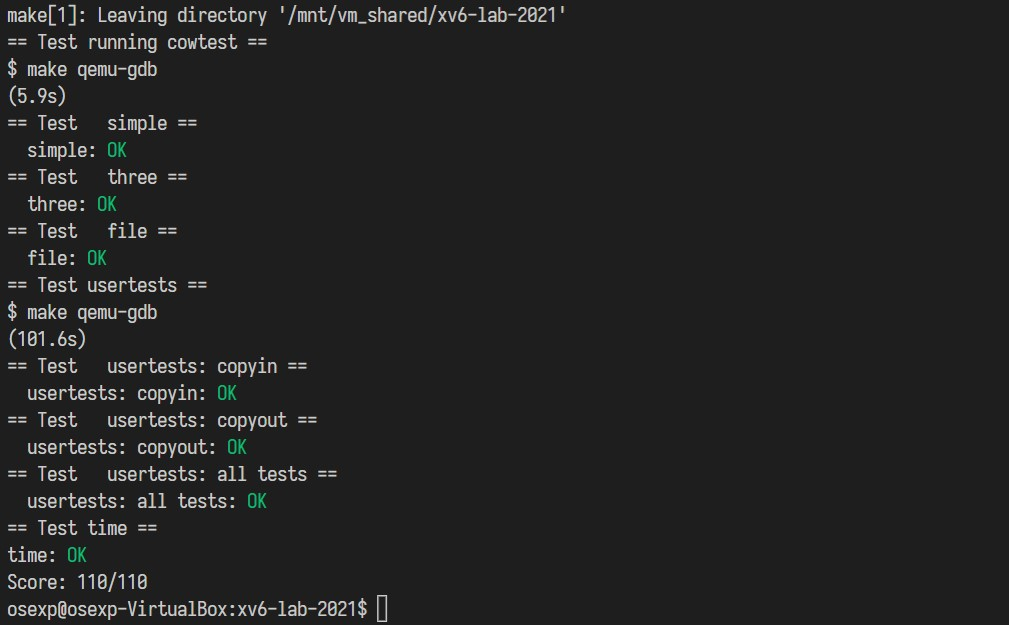
\includegraphics[width=0.8\textwidth]{cow_grade.jpg}
  \caption{ Lab Copy on-write 的测评结果}
\end{figure}
可见测试全部通过,得分为满分。


\section{小结:写时复制(和其它惰性机制)的讨论}

软件工程中有一句重要的论述,出自 Butler Lampson 之手: \textit{All problems in computer science can be solved by another level of indirection.} 通过增加一层中间层,就有了可以引入一些优化机制的空间,这一点不仅在操作系统中极其常见,在其它软件工程的实践中也比比皆是。

在我们本次实验的 COW fork 的例子中,不直接分配页面,而是通过 COW 机制惰性地在程序需要时再分配页面,至少带来了如下几点好处:
\begin{enumerate}
    \item 由于初次 fork 无需真正复制内存, fork 执行地更快
    \item 对于计算密集型的任务,可能子进程无需写内存,故而可以超出物理内存的限制而执行更多的进程
    \item 由于程序局部性原理的存在,即便子进程需要对某些页面进行写入,存放代码段的页面也是父子进程共享的
    \item 共享的内存页面可以大幅度提高处理器中 cache 的效率,提高速度
\end{enumerate}

事实上, COW 机制除了在内存管理中被使用外,在文件系统乃至操作系统外的软件(如数据库)中,也被用于实现一部分的惰性。惰性机制除了 COW 外,我们熟悉的内存交换机制和一些编程语言中提供的惰性求值等,也是惰性机制的体现。惰性机制的核心在于“按需分配”,从而能够避免资源浪费。

避免资源浪费在大多数情况下已经足够优秀了,但在具有更高性能需求的场景,仅仅避免浪费还不够,它们需要系统能够提前准备好程序恰好需要的资源。所以在现代的软件系统中,除了惰性机制,一些基于启发式算法的预测机制也被引入以提高性能。作为惰性机制的反面,提前预测的机制在预测成功时会带来受益,但预测失败则会造成更大的资源浪费与性能损失。在操作系统的层面上,由于预测失败的惩罚较大,故而更多的优化还是从保守的避免浪费的观点出发。
\chapter{Lab Multithreading:多线程实验}
\begin{introduction}
    \item 用户态进程 Uthread
    \item 线程的使用
    \item 线程屏障
    \item 线程、互斥与同步
\end{introduction}

用户态线程作为轻量级的进程,相比于进程有着更加方便的通信机制和更加灵活的使用方法。本次实验的主题是用户态线程,我们将主要在用户态进行线程相关的实验。

\section{用户态进程 Uthread}

在本实验中,我们需要完成一个用户态线程库中的功能。 xv6 为该实验提供了基本的代码: \lstinline{user/uthread.c} 和 \lstinline{user/uthread_switch.S} 。我们需要在 \lstinline{user/uthread.c} 中实现 \lstinline{thread_create()} 和 \lstinline{thread_schedule()} ,并且在 \lstinline{user/uthread_switch.S} 中实现 \lstinline{thread_switch} 用于切换上下文。

首先我们查看 \lstinline{user/uthread.c} 中关于线程的一些数据结构:
\begin{lstlisting}[language=C]
/* Possible states of a thread: */
#define FREE        0x0
#define RUNNING     0x1
#define RUNNABLE    0x2

#define STACK_SIZE  8192
#define MAX_THREAD  4


struct thread {
  char       stack[STACK_SIZE]; /* the thread's stack */
  int        state;             /* FREE, RUNNING, RUNNABLE */
};
struct thread all_thread[MAX_THREAD];
struct thread *current_thread;
\end{lstlisting}

线程的数据结构十分简洁, \lstinline{struct thread} 中,一个字节数组用作线程的栈,一个整数用于表示线程的状态。不难发现我们还需要增加一个数据结构用于保存每个线程的上下文,故参照内核中关于进程上下文的代码,增加以下内容:
\begin{lstlisting}[language=C]
// Saved registers for user context switches.
struct context {
  uint64 ra;
  uint64 sp;

  // callee-saved
  uint64 s0;
  uint64 s1;
  uint64 s2;
  uint64 s3;
  uint64 s4;
  uint64 s5;
  uint64 s6;
  uint64 s7;
  uint64 s8;
  uint64 s9;
  uint64 s10;
  uint64 s11;
};

struct thread {
  char       stack[STACK_SIZE]; /* the thread's stack */
  int        state;             /* FREE, RUNNING, RUNNABLE */
  struct context context;       // uthread_switch() here to switch the thread
};
struct thread all_thread[MAX_THREAD];
struct thread *current_thread;
\end{lstlisting}

参考 xv6 实验手册的提示,除了 sp 、 s0 和 ra 寄存器,我们只需要保存 callee-saved 寄存器,因此构造了上面的 \lstinline{struct context} 结构体。有了该结构体,我们仿照 \lstinline{kernel/trampoline.S} 的结构,按照 \lstinline{struct context} 各项在内存中的位置,在 \lstinline{user/uthread_switch.S} 中加入如下的代码:
\begin{lstlisting}
thread_switch:
	/* YOUR CODE HERE */
	/* Save registers */
    sd ra, 0(a0)
    sd sp, 8(a0)
    sd s0, 16(a0)
    sd s1, 24(a0)
    sd s2, 32(a0)
    sd s3, 40(a0)
    sd s4, 48(a0)
    sd s5, 56(a0)
    sd s6, 64(a0)
    sd s7, 72(a0)
    sd s8, 80(a0)
    sd s9, 88(a0)
    sd s10, 96(a0)
    sd s11, 104(a0)

	/* Restore registers */
    ld ra, 0(a1)
    ld sp, 8(a1)
    ld s0, 16(a1)
    ld s1, 24(a1)
    ld s2, 32(a1)
    ld s3, 40(a1)
    ld s4, 48(a1)
    ld s5, 56(a1)
    ld s6, 64(a1)
    ld s7, 72(a1)
    ld s8, 80(a1)
    ld s9, 88(a1)
    ld s10, 96(a1)
    ld s11, 104(a1)
	ret    /* return to ra */
\end{lstlisting}

这样就完成了上下文切换的功能,接下来需要完成创建线程和调度线程的部分。创建线程时,我们需要将线程的栈设置好,并且需要保证在线程被调度运行时能够将 pc 跳转到正确的位置。上面的 \lstinline{thread_switch} 在保存第一个进程的上下文后会加载第二个进程的上下文,然后跳至刚刚加载的 ra 地址处开始执行,故而我们在创建进程时只需将 ra 设为我们所要执行的线程的函数地址即可。于是 \lstinline{thread_create()} 的实现如下:
\begin{lstlisting}[language=C]
void 
thread_create(void (*func)())
{
  struct thread *t;

  for (t = all_thread; t < all_thread + MAX_THREAD; t++) {
    if (t->state == FREE) break;
  }
  t->state = RUNNABLE;
  // YOUR CODE HERE
  t->context.ra = (uint64)func;
  t->context.sp = (uint64)&t->stack[STACK_SIZE];
}
\end{lstlisting}

类似的,在调度线程时,我们选中下一个可运行的线程后,使用 \lstinline{thread_switch} 切换上下文即可,实现如下:
\begin{lstlisting}[language=C]
void 
thread_schedule(void)
{
......
    /* YOUR CODE HERE
     * Invoke thread_switch to switch from t to next_thread:
     * thread_switch(??, ??);
     */
    // t->state = RUNNABLE;
    thread_switch((uint64)&t->context, (uint64)&current_thread->context);
......
}
\end{lstlisting}

\begin{theorem}[为何调度时不将原有线程的状态改为 RUNNABLE]
    这里一个常见的错误是在调度时很自然地将原有线程的状态改为 RUNNABLE 。事实上,由于本实验中的线程是主动让出的非抢占式调度,在线程主动让出 CPU 时调用的 \lstinline{thread_yield()} 中已经进行了状态的改变,故而此处无需对原线程状态进行修改。若在 \lstinline{thread_schedule()} 中执行 \lstinline{t->state = RUNNABLE} ,则会导致初始化用的 0 号线程也被多次唤醒,导致调度上的错误。
\end{theorem}

这样便完成了线程库的基本功能。编译运行 xv6 ,然后执行 \lstinline{uthread} ,便可看到各线程井然有序地执行,如下图所示:
\begin{figure}[H]
  \centering
  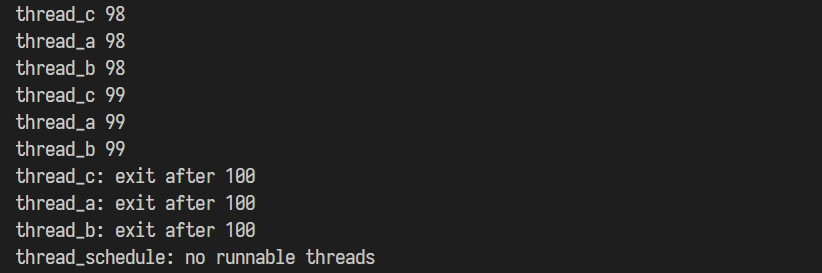
\includegraphics[width=0.8\textwidth]{thread_uthread.jpg}
  \caption{ \lstinline{uthread} 的执行结果}
\end{figure}
说明该用户态线程库的实现是正确的。

\section{线程的使用}

本部分的第二个实验不涉及到 xv6 ,而是在常规的拥有多核的 Linux 机器下进行(需要将我们的虚拟机的 CPU 数量调整为大于 1 的值),使用著名的 \lstinline{pthread} 库来研究多线程中的一些问题。本实验中,我们需要修改 \lstinline{notxv6/ph.c} ,使之在多线程读写一个哈希表的情况下能够产生正确的结果。

首先运行 \lstinline{make ph} 编译 \lstinline{notxv6/ph.c} ,运行 \lstinline{./ph 1} ,可以获得类似下面输出:
\begin{lstlisting}
    100000 puts, 3.991 seconds, 25056 puts/second
    0: 0 keys missing
    100000 gets, 3.981 seconds, 25118 gets/second
\end{lstlisting}

不难发现,写入哈希表的数据被完整地读出,没有遗漏。然后运行 \lstinline{./ph 2} ,则输出如下:
\begin{lstlisting}
    100000 puts, 1.885 seconds, 53044 puts/second
    1: 16579 keys missing
    0: 16579 keys missing
    200000 gets, 4.322 seconds, 46274 gets/second
\end{lstlisting}

在多线程同时读写的情况下,部分数据由于竞争访问,一些数据没有被正确写入到哈希表中,因而我们需要解决这个问题。一个常规的解决方案是给共享数据结构加上锁,获得锁的线程才可以写该数据结构。查阅 \lstinline{man pthreads} 和其它关于 \lstinline{pthread} 的线程加锁的资料后,我们首先定义一个保护哈希表的互斥锁:
\begin{lstlisting}[language=C]
......
    pthread_mutex_t lock;
......
\end{lstlisting}
然后在开始线程前对其进行初始化:
\begin{lstlisting}[language=C]
    pthread_mutex_init(&lock, NULL);
\end{lstlisting}
最后在写入操作哈希表时加上获取锁的操作,并在写入完成后释放锁:
\begin{lstlisting}[language=C]
static 
void put(int key, int value)
{
......
    // the new is new.
    pthread_mutex_lock(&lock);
    insert(key, value, &table[i], table[i]);
    pthread_mutex_unlock(&lock);
......  
}
\end{lstlisting}

此时再使用  \lstinline{make ph} 编译 \lstinline{notxv6/ph.c} ,运行 \lstinline{./ph 2} ,则发现没有读出的数据缺失,如下图所示:
\begin{figure}[H]
  \centering
  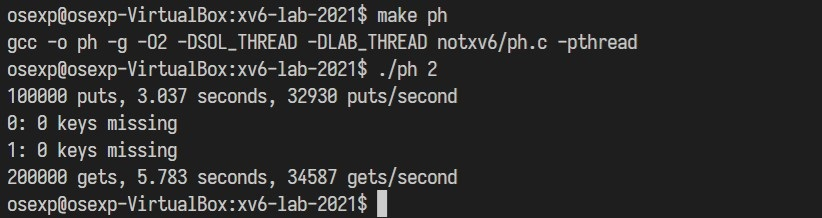
\includegraphics[width=0.8\textwidth]{thread_ph.jpg}
  \caption{ \lstinline{./ph 2} 的执行结果}
\end{figure}

\begin{proposition}[为何读时不加锁] 
    事实上,我们在一些对于数据一致性要求较高的程序(如数据库)中,一个线程在读取数据时,如果不对相应的资源加锁,则可能读到过时或“脏”的数据,这个现象在数据库中被称为“幻读”。数据库根据其需求,设置了各种隔离级别,只有在较高的隔离级别上才会使用加锁或完全串行化操作的方式解决幻读等问题。在上面的 \lstinline{ph} 程序中,由于不涉及到对数据的并发修改或删除,故而在读取时无需加锁。
\end{proposition}

\section{线程屏障}

除了锁以外,线程屏障 \lstinline{barrier} 也是线程进行同步的重要机制。线程屏障 \lstinline{barrier} 可以看成线程的检查点,即某个参与 \lstinline{barrier} 的线程先执行到 \lstinline{barrier()} 语句处时,其需要等待其它尚未到达 \lstinline{barrier()} 处的线程;当所有参与线程屏障的线程都到达 \lstinline{barrier()} 语句处时,所有参与线程屏障的线程都继续运行。

首先运行 \lstinline{make barrier} 编译 \lstinline{notxv6/barrier.c} ,运行 \lstinline{./barrier 2} ,可以获得类似下面输出:
\begin{lstlisting}
    $ make barrier
    $ ./barrier 2
    barrier: notxv6/barrier.c:42: thread: Assertion `i == t' failed.
\end{lstlisting}
说明该 \lstinline{barrier()} 并未正确实现。

根据 xv6 实验手册中的提示,可以使用条件变量来实现 \lstinline{barrier} 机制。首先查看 \lstinline{barrier.c} 中相关的数据结构:
\begin{lstlisting}[language=C]
    struct barrier {
        pthread_mutex_t barrier_mutex;
        pthread_cond_t barrier_cond;
        int nthread;      // Number of threads that have reached this round of the barrier
        int round;     // Barrier round
      } bstate;
\end{lstlisting}

为实现线程屏障,需要维护一个互斥锁、一个条件变量、用以记录到达线程屏障的线程数的整数和记录线程屏障轮数的整数。在初始化用的 \lstinline{barrier_init()} 中,互斥锁、条件变量及 \lstinline{nthread} 被初始化。此后在某个线程到达 \lstinline{barrier()} 时,需要获取互斥锁进而修改 \lstinline{nthread}。当 \lstinline{nthread} 与预定的值相等时,将 \lstinline{nthread} 清零,轮数加一,并唤醒所有等待中的线程。最后不要忘记在 \lstinline{barrier()} 中释放互斥锁。笔者的实现如下所示:
\begin{lstlisting}[language=C]
static void 
barrier()
{
  // YOUR CODE HERE
  pthread_mutex_lock(&bstate.barrier_mutex);
  bstate.nthread ++;
  if (bstate.nthread == nthread)
  {
    bstate.round++;
    bstate.nthread = 0;
    pthread_cond_broadcast(&bstate.barrier_cond);
  } else {
    pthread_cond_wait(&bstate.barrier_cond, &bstate.barrier_mutex);
  }
  pthread_mutex_unlock(&bstate.barrier_mutex);
}
\end{lstlisting}

此时使用 \lstinline{make barrier} 编译 \lstinline{notxv6/barrier.c} ,运行 \lstinline{./barrier 2} ,则通过测试,如下图所示:
\begin{figure}[H]
  \centering
  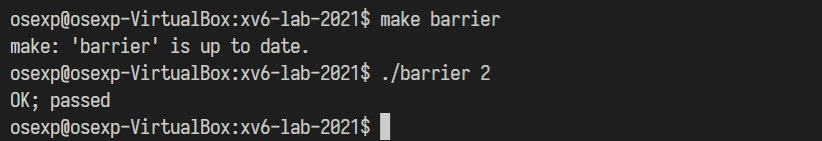
\includegraphics[width=0.8\textwidth]{thread_barrier.jpg}
  \caption{ \lstinline{./barrier 2} 的执行结果}
\end{figure}

\paragraph*{实验结果} 在完成 Lab Multithreading 中的所有实验后,根据 MIT 6.S081 的传统,需要在实验目录下创建一个名为 \lstinline{time.txt} 文本文件,其中只包含一行,为完成该实验的小时数。然后在终端中执行 \lstinline{make grade} ,即可对整个实验进行自动评分,笔者的结果如下:
\begin{figure}[H]
  \centering
  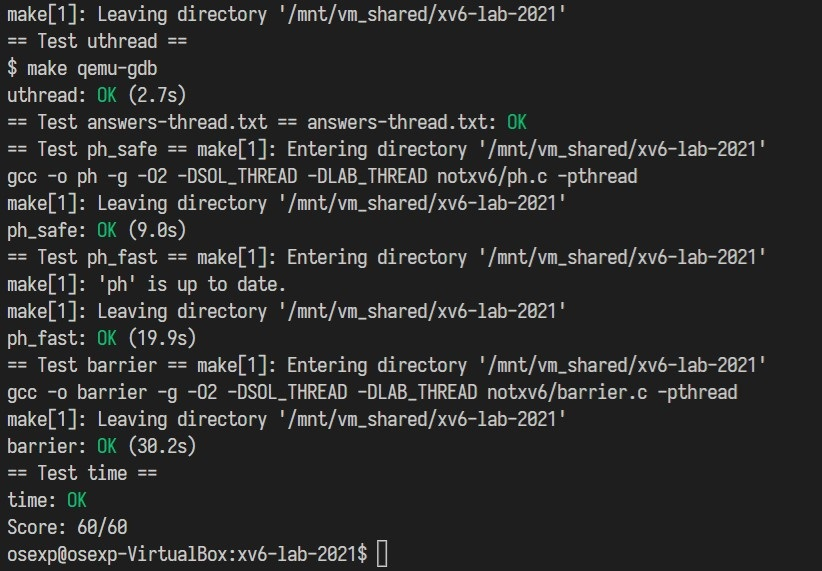
\includegraphics[width=0.8\textwidth]{thread_grade.jpg}
  \caption{ Lab Multithreading 的测评结果}
\end{figure}
可见测试全部通过,得分为满分。

\section{小结:线程、互斥与同步}

Lab Multithreading 中的三个实验并不困难,但是其十分准确地阐释了线程的三个重要概念:上下文切换、互斥与同步。

上下文的切换需要设计存储上下文的数据结构,并在用户态结合 ABI 的规范及使用汇编实现切换程序,从而保存并设置各寄存器(重要的是 ra 和 sp 寄存器)。

由于各线程共享内存空间,在可能发生数据的竞争写入等需要线程互斥的场景,一般使用线程库提供的互斥锁实现线程的互斥。

各线程协作时,可能需要在代码执行到某个位置时使得线程同步,在本部分的实验中,使用条件变量实现的 \lstinline{barrier} 来进行线程同步。

此外,由于线程共享内存空间的特性,线程间通信并不需要特殊的讨论,只需利用内存中共享的数据结构即可完成通信(例如带锁的全局变量等)。


\chapter{Lab network driver:网卡驱动实验}
\begin{introduction}
    \item 实现 Intel E1000 网卡的驱动
    \item 编写驱动程序的一般步骤
\end{introduction}

驱动程序是操作系统的重要组成部分,负责沟通操作系统和实际工作的硬件。在本次实验中,我们会在 xv6 中为一个现实中广泛使用的硬件: Intel E1000 网卡,编写驱动程序,从而体会编写驱动程序的一般步骤。

\section{实现 Intel E1000 网卡的驱动}

Intel E1000 网卡是一类常见的千兆以太网卡,广泛用于各类个人电脑和服务器中。由于其支持较为完善,且文档齐全,故而在我们的 qemu 中也有软件模拟的 E1000 设备,可供 xv6 实验使用。

在开始编写驱动程序前,我们需要获取 Intel 提供的关于 E1000 网卡的驱动的开发者文档 \textit{Intel E1000 Software Developer's Manual} \footnote{\url{https://pdos.csail.mit.edu/6.828/2021/readings/8254x_GBe_SDM.pdf}} ,其中包含了关于该网卡硬件特性和工作机制的说明。根据 xv6 的实验手册,我们主要需要关注以下内容:
\begin{enumerate}
    \item Section 2 :关于 E1000 的基本信息
    \item Section 3.2 :接收数据包的简介
    \item Section 3.3 和 Section 3.4 :发送数据包的简介
    \item Section 13 : E1000 使用到的寄存器
    \item Section 14 : E1000 的设备初始化过程
\end{enumerate}

大致浏览过上面的内容后,我们主要需要实现 \lstinline{kernel/e1000.c} 中的两个函数: 用于发送数据包的 \lstinline{e1000_transmit()} 和用于接收数据包的 \lstinline{e1000_recv()} 。用于初始化设备的 \lstinline{e1000_init()} 已经被实现好了,我们主要关注的是其涉及到的一些数据结构:
\begin{lstlisting}[language=C]
    #define TX_RING_SIZE 16
    static struct tx_desc tx_ring[TX_RING_SIZE] __attribute__((aligned(16)));
    static struct mbuf *tx_mbufs[TX_RING_SIZE];
    
    #define RX_RING_SIZE 16
    static struct rx_desc rx_ring[RX_RING_SIZE] __attribute__((aligned(16)));
    static struct mbuf *rx_mbufs[RX_RING_SIZE];
    
    // remember where the e1000's registers live.
    static volatile uint32 *regs;
    
    struct spinlock e1000_lock;
\end{lstlisting}

其中最重要的是两个环形缓冲区: \lstinline{tx_ring} 和 \lstinline{rx_ring} 。根据 \textit{Intel E1000 Software Developer's Manual} 上的描述,我们只需要将需要发送的数据包放入环形缓冲区中,设置好对应的参数并更新管理缓冲区的寄存器,即可视为完成了数据包的发送。此后网卡的硬件会自动在合适的时间将我们放入的数据包按照配置发送出去,在 \lstinline{kernel/e1000.c} 中的实现如下:
\begin{lstlisting}[language=C]
int
e1000_transmit(struct mbuf *m)
{
  //
  // Your code here.
  acquire(&e1000_lock);
  printf("e1000_transmit: called mbuf=%p\n",m);
  uint32 idx = regs[E1000_TDT]; 
  if (tx_ring[idx].status != E1000_TXD_STAT_DD)
  {
    __sync_synchronize();
    release(&e1000_lock);
    return -1;
  } else {
    if (tx_mbufs[idx] != 0)
    {
      mbuffree(tx_mbufs[idx]);
    }
    tx_ring[idx].addr = (uint64) m->head;
    tx_ring[idx].length = (uint16) m->len;
    tx_ring[idx].cso = 0;
    tx_ring[idx].css = 0;
    tx_ring[idx].cmd = 1;
    tx_mbufs[idx] = m;
    regs[E1000_TDT] = (regs[E1000_TDT] + 1) % TX_RING_SIZE;
  }
  release(&e1000_lock);
  return 0;
}
\end{lstlisting}

\begin{theorem}[关于锁和\lstinline{__sync_synchronize}]
    由于网卡本身就是仅有一份、只能独占的资源,故而对其进行操作时需要加锁。但在上面的代码中,当缓冲区满时,我们加入了一行 \lstinline{__sync_synchronize()} ,简单来说,其起到内存屏障的作用,即保证对内存的操作严格按照我们指定的顺序进行。若没有这个语句,则在发包缓冲区满时会出现一些难以调试的错误。
\end{theorem}

对于 \lstinline{e1000_recv()} 也依样画瓢,只是在将数据包拷贝出 \lstinline{rx_ring} 时,需要使用合适的函数。根据 xv6 实验手册的提示,我们无需自己实现该拷贝过程,而只需要调用 \lstinline{net.c} 中的 \lstinline{net_rx()} 即可。注意当网卡硬件产生一次中断后,我们的中断处理过程 \lstinline{e1000_intr} 会执行 \lstinline{regs[E1000_ICR] = 0xffffffff} 从而告知网卡我们已经完成了这次中断中所有数据包的处理,故而我们的 \lstinline{e1000_recv()} 需要将 \lstinline{rx_ring} 中的所有内容都拷贝出去,实现如下:
\begin{lstlisting}[language=C]
extern void net_rx(struct mbuf *);
static void
e1000_recv(void)
{
  //
  // Your code here.
  uint32 idx = (regs[E1000_RDT] + 1) % RX_RING_SIZE;
  struct rx_desc* dest = &rx_ring[idx];
  while (rx_ring[idx].status & E1000_RXD_STAT_DD)
  {
    acquire(&e1000_lock);

    struct mbuf *buf = rx_mbufs[idx];
    mbufput(buf, dest->length);
    if (!(rx_mbufs[idx] = mbufalloc(0)))
      panic("mbuf alloc failed");
    dest->addr = (uint64)rx_mbufs[idx]->head;
    dest->status = 0;
    regs[E1000_RDT] = idx;

    __sync_synchronize();
    release(&e1000_lock);
    net_rx(buf);
    idx = (regs[E1000_RDT] + 1) % RX_RING_SIZE;
    dest = &rx_ring[idx];
  }
}
\end{lstlisting}

这里同样需要加锁保证互斥,并使用 \lstinline{__sync_synchronize} 保证内存访问顺序,否则会使接收数据包的顺序产生变化。

至此,在 E1000 中我们需要做的工作便完成了。使用 \lstinline{make server} 运行 qemu 宿主机的服务器,然后用 \lstinline{make qemu} 编译并启动 xv6 ,在 xv6 中运行 \lstinline{nettests} ,可以得到如下图的结果:
\begin{figure}[H]
  \centering
  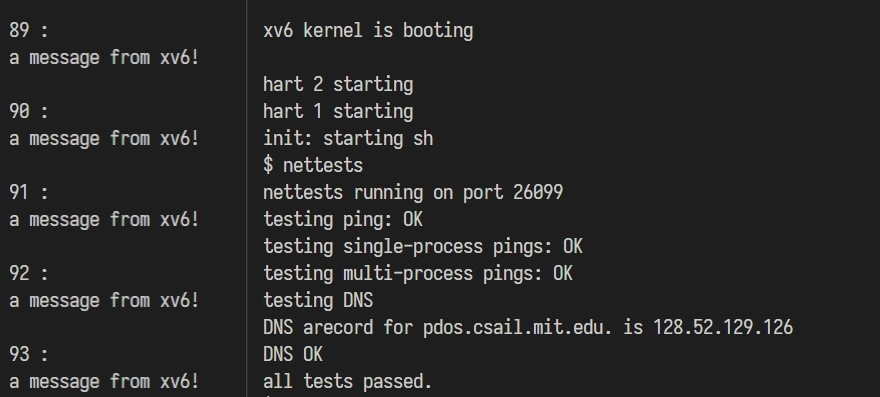
\includegraphics[width=0.8\textwidth]{net_nettests.jpg}
  \caption{网卡驱动的测试结果}
\end{figure}

可见结果符合预期。

\begin{proposition}[关于 DMA] 
    这里的 E1000 网卡驱动就是一个典型的使用 DMA ( Direct Memory Access ,直接存储器访问)的例子。网卡在初始化配置好后,会将收到的数据包和关于这些数据包的信息直接拷贝到内存的指定位置中,而无需 CPU 的参与。当网卡认为有必要让 CPU 处理这些数据时,就使用设备中断的方式通知 CPU 。从编写程序的角度看,我们并没有书写任何直接从网卡拷贝数据的代码,但对应的数据结构中已经被填充完成了;处理好一次中断收到的数据后,只要设置对应的寄存器,就可以告知网卡我们已经妥善处理其通过 DMA 传入的数据。
\end{proposition}

\paragraph*{实验结果} 在完成 Lab network driver 中的所有实验后,根据 MIT 6.S081 的传统,需要在实验目录下创建一个名为 \lstinline{time.txt} 文本文件,其中只包含一行,为完成该实验的小时数。先打开一个终端,在其中使用 \lstinline{make server} 运行 qemu 宿主机的服务器;然后打开另一个终端,在其中执行 \lstinline{make grade} ,即可对整个实验进行自动评分,笔者的结果如下:
\begin{figure}[H]
  \centering
  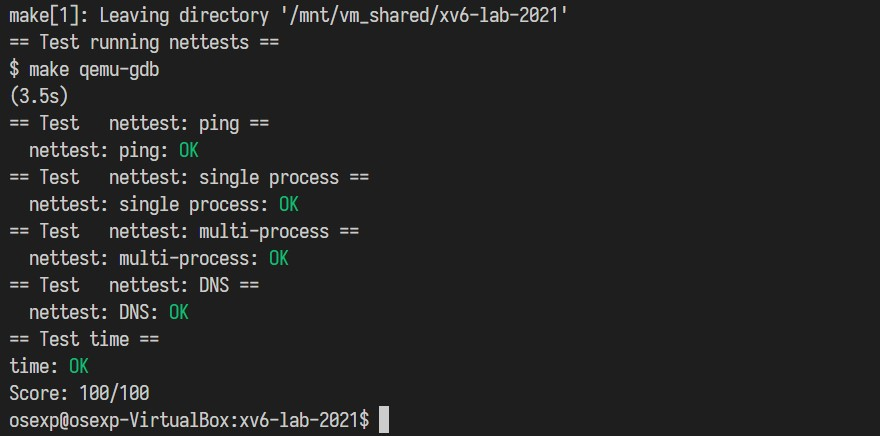
\includegraphics[width=0.8\textwidth]{net_grade.jpg}
  \caption{ Lab network driver 的测评结果}
\end{figure}
可见测试全部通过,得分为满分。

\section{小结:编写驱动程序的一般步骤}

由于现代大多数外设都通过 DMA 方式来与系统进行数据交换,故而很多外设驱动的编写的思路和本部分实验的一致。这里我们对编写驱动程序的一般步骤进行小结:
\begin{enumerate}
    \item 获取设备相关的文档
    \item 了解设备工作的大致过程
    \item 设计与设备交换数据的数据结构
    \item 创建对应的内核模块
    \item 编写设备初始化代码
    \item 编写具体功能
    \item 测试与验证
\end{enumerate}
\chapter{Lab Lock:锁的实验}
\begin{introduction}
    \item 实现每个 CPU 独占的内存分配器
    \item 实现 IO 缓存
    \item 减少加锁开销
\end{introduction}

前面的很多实验中都涉及到了加锁的问题。锁作为一种互斥机制,对于开发者而言实现简单,理解其行为也不复杂,且能提供可靠的互斥保障。但过多的加锁操作会显著地降低系统的并行性,从而使得多处理机系统无法发挥其应有的性能。本部分实验中,主要涉及对于加锁机制的优化,从而增加 xv6 内核的并行性。

\section{实现每个 CPU 独占的内存分配器}

在这个实验中, xv6 提供了用户态程序 \lstinline{kalloctest} ,用于对 xv6 的内存分配器进行压力测试。用户态程序 \lstinline{kalloctest} 产生三个进程,这些进程会不断分配并释放内存,使得原始的 xv6 中的只有一个空闲链表的数据结构的锁被不断获取和释放,且大多数时候对锁的 \lstinline{acquire()} 会被阻塞。用户态程序 \lstinline{kalloctest} 会统计 \lstinline{acquire()} 时被阻塞消耗的循环次数,用以估计加锁产生的额外开销。

在我们没有改进 xv6 的内存分配器之前,编译并运行 xv6 ,然后运行 \lstinline{kalloctest} ,会得到类似下面的结果:
\begin{lstlisting}
    $ kalloctest
    start test1
    test1 results:
    --- lock kmem/bcache stats
    lock: kmem: #fetch-and-add 83375 #acquire() 433015
    lock: bcache: #fetch-and-add 0 #acquire() 1260
    --- top 5 contended locks:
    lock: kmem: #fetch-and-add 83375 #acquire() 433015
    lock: proc: #fetch-and-add 23737 #acquire() 130718
    lock: virtio_disk: #fetch-and-add 11159 #acquire() 114
    lock: proc: #fetch-and-add 5937 #acquire() 130786
    lock: proc: #fetch-and-add 4080 #acquire() 130786
    tot= 83375
    test1 FAIL
\end{lstlisting}

可见 \lstinline{acquire()} 时被阻塞消耗的循环的计数十分巨大,说明内存分配时等待获取锁会浪费大量时间,从而使得内存分配的效率较低。

根据 xv6 手册的提示,一种降低加锁引起的开销的方法是为每一个 CPU 核心设置一个单独的空闲链表和对应的锁,这样运行在某 CPU 上的进程在试图分配内存时,会获取自己所在的 CPU 上空闲链表的锁然后尝试分配内存,只有当无法分配内存时,内存分配器才会到其它 CPU 的空闲链表中借取空闲的页面。

\begin{proposition}[资源重复设置与减小加锁开销] 
    从另一个角度看,这里为每个 CPU 设置一个内存分配器属于资源的重复设置。通过重复设置资源,可以使得进程直接获得锁而无需等待的概率大大提高,从而降低了进程等待时间的期望值,故整个系统的效率能够得到提高。但是,资源重复设置可能会引起诸如数据一致性等问题,故而会大大增加软件的复杂度。
\end{proposition}

首先,我们修改 \lstinline{kalloc.c} 中的数据结构,使单一的空闲链表变为多个空闲链表的数组:
\begin{lstlisting}[language=C]
    struct {
        struct spinlock lock;
        struct run *freelist;
      } kmem[NCPU];
\end{lstlisting}

然后,我们需要根据上面的分配与释放的逻辑,对 \lstinline{kalloc()} 进行修改。首先需要利用 \lstinline{cpuid()} 读取特殊寄存器以获得当前运行的 CPU 的编号,该编号对应着一个空闲链表,在获取该编号时需要关闭中断,以免发生不测。
\begin{lstlisting}[language=C]
void *
kalloc(void)
{
  struct run *r;
  push_off();
  int c = cpuid();
  pop_off();
......
\end{lstlisting}

成功获取 CPU 编号后,我们需要获取对应的空闲链表的锁,然后试图分配页面:
\begin{lstlisting}[language=C]
......
  acquire(&kmem[c].lock);
  r = kmem[c].freelist;
  if(r)
  {
    kmem[c].freelist = r->next;
    release(&kmem[c].lock);
......
\end{lstlisting}

若该 CPU 的空闲链表中没有空闲页面,则到其它 CPU 中借用一个:
\begin{lstlisting}[language=C]
......
} else {
    release(&kmem[c].lock);
    for (int i = 0; i<NCPU; i++)
    {
      acquire(&kmem[i].lock);
      r = kmem[i].freelist;
      if(r)
      {
        kmem[i].freelist = r->next;
        release(&kmem[i].lock);
        break;
      } else {
        release(&kmem[i].lock);
      }
    }
  }
......
\end{lstlisting}

最后若分配成功,则返回获取的页面,笔者完整的实现如下:
\begin{lstlisting}[language=C]
void *
kalloc(void)
{
  struct run *r;
  push_off();
  int c = cpuid();
  pop_off();

  acquire(&kmem[c].lock);
  r = kmem[c].freelist;
  if(r)
  {
    kmem[c].freelist = r->next;
    release(&kmem[c].lock);
  } else {
    release(&kmem[c].lock);
    for (int i = 0; i<NCPU; i++)
    {
      acquire(&kmem[i].lock);
      r = kmem[i].freelist;
      if(r)
      {
        kmem[i].freelist = r->next;
        release(&kmem[i].lock);
        break;
      } else {
        release(&kmem[i].lock);
      }
    }
  }
  if(r)
    memset((char*)r, 5, PGSIZE);  // fill with junk
  return (void*)r;
}
\end{lstlisting}

对分配内存的 \lstinline{kalloc()} 修改完成后,我们还需要修改对应的用于释放内存的 \lstinline{kfree()} ,直接将页面加入到当前的 CPU 空闲链表中(即便是借来的页面,也不归还了),实现如下:
\begin{lstlisting}[language=C]
void
kfree(void *pa)
{
  struct run *r;
  push_off();
  int c = cpuid();
  pop_off();

  if(((uint64)pa % PGSIZE) != 0 || (char*)pa < end || (uint64)pa >= PHYSTOP)
    panic("kfree");

  // Fill with junk to catch dangling refs.
  memset(pa, 1, PGSIZE);

  r = (struct run*)pa;

  acquire(&kmem[c].lock);
  r->next = kmem[c].freelist;
  kmem[c].freelist = r;
  release(&kmem[c].lock);
}
\end{lstlisting}

最后不要忘记初始化内存分配器的 \lstinline{kinit()} ,其需要初始化每个 CPU 的空闲链表和锁:
\begin{lstlisting}[language=C]
void
kinit()
{
  for (int i = 0; i<NCPU; i++)
  {
    initlock(&kmem[i].lock, "kmem");
  }
  freerange(end, (void*)PHYSTOP);
}
\end{lstlisting}

调用 \lstinline{freerange} 的 CPU 会在初始化时获得所有的空闲页面,不过无需担心分配不均,这些页面会在一次次的 \lstinline{kalloc()} 和 \lstinline{kfree()} 的过程中进入其它 CPU 的空闲链表中。

至此,对于 xv6 的内存分配器的改造已经完成,再次编译并运行 xv6 ,然后运行 \lstinline{kalloctest} ,会得到类似下图的结果:
\begin{figure}[H]
  \centering
  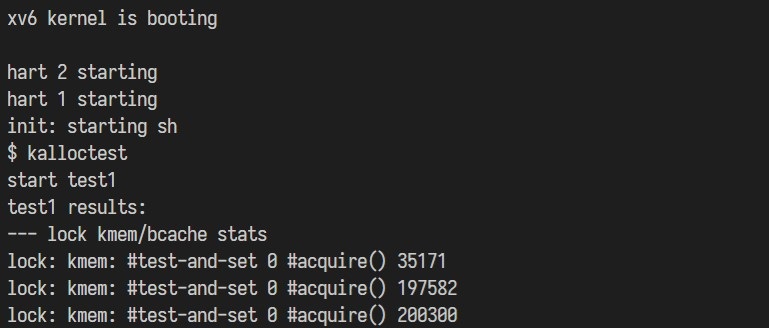
\includegraphics[width=0.8\textwidth]{lock_kalloctest.jpg}
  \caption{ \lstinline{kalloctest} 的测试结果}
\end{figure}
最后 \lstinline{kalloctest} 输出 \lstinline{test0 OK} 、 \lstinline{test1 OK} 和 \lstinline{test2 OK},且加锁开销远小于改进前的值,符合我们的预期。

\section{实现 IO 缓存}

由于磁盘等外存设备普遍读写速度较慢,故很多操作系统都会在其文件系统的机制中设置外存块的缓存,以提高整个系统的性能。在 xv6 中也有类似的机制,在 \lstinline{bio.c} 中可以看到其实现。

在原始的 xv6 中,对于缓存的读写是由单一的锁 \lstinline{bcache.lock} 来保护的,这就导致了如果系统中有多个进程在进行 IO 操作,则等待获取 \lstinline{bcache.lock} 的开销就会较大。为了减少加锁的开销, xv6 的实验手册提示我们可以将缓存分为几个桶,为每个同单独设置一个锁,这样如果两个进程访问的缓存块在不同的桶中,则可以同时获得两个锁从而进行操作,而无需等待加锁。我们的目标是将 \lstinline{bcachetest} 中统计值 \lstinline{tot} 降到规定值以下,在没有改进前, xv6 中运行 \lstinline{bcachetest} 的结果大致如下:
\begin{lstlisting}
    $ bcachetest
    start test0
    test0 results:
    --- lock kmem/bcache stats
    lock: kmem: #fetch-and-add 0 #acquire() 33035
    lock: bcache: #fetch-and-add 16142 #acquire() 65978
    --- top 5 contended locks:
    lock: virtio_disk: #fetch-and-add 162870 #acquire() 1188
    lock: proc: #fetch-and-add 51936 #acquire() 73732
    lock: bcache: #fetch-and-add 16142 #acquire() 65978
    lock: uart: #fetch-and-add 7505 #acquire() 117
    lock: proc: #fetch-and-add 6937 #acquire() 73420
    tot= 16142
    test0: FAIL
    start test1
    test1 OK
\end{lstlisting}


依照上面的思想,我们首先改造 \lstinline{bcache} 的数据结构,将单个锁改成多个锁,并将缓存块分组:
\begin{lstlisting}[language=C]
    struct {
        struct spinlock lock[NBUCKET];
        struct buf buf[NBUF];

        struct buf bucket[NBUCKET];
      } bcache;
\end{lstlisting}

然后,修改对应的一些头文件中的定义,如在 \lstinline{param.h} 中:
\begin{lstlisting}[language=C]
    #define NBUF         (MAXOPBLOCKS*12)  // size of disk block cache
\end{lstlisting}
在 \lstinline{defs.h} 中:
\begin{lstlisting}[language=C]
    int             can_lock(int, int);
\end{lstlisting}

在 \lstinline{buf.h} 中:
\begin{lstlisting}[language=C]
    struct buf {
        int valid;   // has data been read from disk?
        int disk;    // does disk "own" buf?
        uint dev;
        uint blockno;
        struct sleeplock lock;
        uint refcnt;
        struct buf *prev; // LRU cache list
        struct buf *next;
        uchar data[BSIZE];
        uint time;
      };
\end{lstlisting}

然后,修改对应的 \lstinline{bcache} 初始化函数 \lstinline{binit()} ,使之与修改后的数据结构相适应:
\begin{lstlisting}[language=C]
void binit(void)
{
  struct buf *b;

  for (int i = 0; i < NBUCKET; i++)
  {
    initlock(&bcache.lock[i], "bcache.bucket");
  }
  b = &bcache.bucket[0];
  for (int i = 0; i < NBUF; i++)
  {
    b->next = &bcache.buf[i];
    b = b->next;
    initsleeplock(&b->lock, "buffer");
  }
}
\end{lstlisting}

之后构建一个辅助函数 \lstinline{can_lock()} ,用于避免死锁:
\begin{lstlisting}[language=C]
int can_lock(int cur_idx, int req_idx)
{
  int mid = NBUCKET / 2;
  // non-reentrant
  if (cur_idx == req_idx)
  {
    return 0;
  }
  else if (cur_idx < req_idx)
  {
    if (req_idx <= (cur_idx + mid))
    {
      return 0;
    }
  }
  else
  {
    if (cur_idx >= (req_idx + mid))
    {
      return 0;
    }
  }
  return 1;
}
\end{lstlisting}

然后改造 \lstinline{bget()} ,按照上面提到的逻辑,将原来的集中管理改为分桶进行管理:
\begin{lstlisting}[language=C]
static struct buf *
bget(uint dev, uint blockno)
{
  int bucket_id = blockno % NBUCKET;
  struct buf *b;

  acquire(&bcache.lock[bucket_id]);
  b = bcache.bucket[bucket_id].next;
  while (b)
  {
    if (b->dev == dev && b->blockno == blockno)
    {
      b->refcnt++;
      release(&bcache.lock[bucket_id]);
      acquiresleep(&b->lock);
      return b;
    }
    b = b->next;
  }
  int index = -1;
  uint min_tick = 0xffffffff;
  for (int j = 0; j < NBUCKET; j++)
  {
    if (!can_lock(bucket_id, j))
    {
      continue;
    }
    else
    {
      acquire(&bcache.lock[j]);
    }
    b = bcache.bucket[j].next;
    while (b)
    {
      if (b->refcnt == 0)
      {
        if (b->time < min_tick)
        {
          min_tick = b->time;
          if (index != -1 && index != j && holding(&bcache.lock[index]))
          {
            release(&bcache.lock[index]);
          }
          index = j;
        }
      }
      b = b->next;
    }
    if (j != index && holding(&bcache.lock[j]))
    {
      release(&bcache.lock[j]);
    }
  }

  if (index == -1)
  {
    panic("bget: no buffers");
  }

  struct buf *move = 0;
  b = &bcache.bucket[index];
  while (b->next)
  {
    if (b->next->refcnt == 0 && b->next->time == min_tick)
    {
      b->next->dev = dev;
      b->next->blockno = blockno;
      b->next->valid = 0;
      b->next->refcnt = 1;
      // remove buf from the old bucket
      move = b->next;
      b->next = b->next->next;
      release(&bcache.lock[index]);
      break;
    }
    b = b->next;
  }
  b = &bcache.bucket[bucket_id];
  while (b->next)
  {
    b = b->next;
  }
  move->next = 0;
  b->next = move;
  release(&bcache.lock[bucket_id]);
  acquiresleep(&move->lock);
  return move;
}

\end{lstlisting}

对应的 \lstinline{brelse} 也要进行修改:
\begin{lstlisting}[language=C]
void brelse(struct buf *b)
{
  if (!holdingsleep(&b->lock))
    panic("brelse");

  releasesleep(&b->lock);

  int bucket_id = b->blockno % NBUCKET;
  acquire(&bcache.lock[bucket_id]);
  b->refcnt--;
  if (b->refcnt == 0)
  {
    b->time = ticks;
  }
  release(&bcache.lock[bucket_id]);
}
\end{lstlisting}

最后发现还有两个函数与 \lstinline{bcache} 的操作相关,一并进行修改:
\begin{lstlisting}[language=C]
void bpin(struct buf *b)
{
  int bucket_id = b->blockno % NBUCKET;
  acquire(&bcache.lock[bucket_id]);
  b->refcnt++;
  release(&bcache.lock[bucket_id]);
}

void bunpin(struct buf *b)
{
  int bucket_id = b->blockno % NBUCKET;
  acquire(&bcache.lock[bucket_id]);
  b->refcnt--;
  release(&bcache.lock[bucket_id]);
}
\end{lstlisting}

此时对 \lstinline{bcache} 的改进基本完成,再次编译并运行 xv6 ,然后运行 \lstinline{bcachetest} ,会得到类似下图的结果:
\begin{figure}[H]
  \centering
  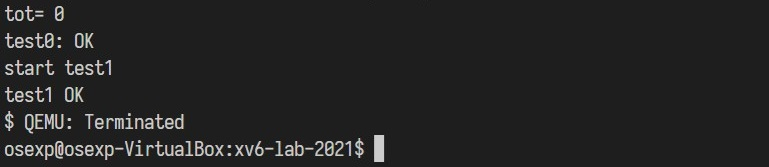
\includegraphics[width=0.8\textwidth]{lock_bcachetest.jpg}
  \caption{ \lstinline{bcachetest} 的测试结果}
\end{figure}
最后 \lstinline{bcachetest} 输出 \lstinline{test0 OK} 和 \lstinline{test1 OK},且加锁开销远小于改进前的值,符合我们的预期。

\paragraph*{实验结果} 在完成 Lab Lock 中的所有实验后,根据 MIT 6.S081 的传统,需要在实验目录下创建一个名为 \lstinline{time.txt} 文本文件,其中只包含一行,为完成该实验的小时数。然后在终端中执行 \lstinline{make grade} ,即可对整个实验进行自动评分,笔者的结果如下:
\begin{figure}[H]
  \centering
  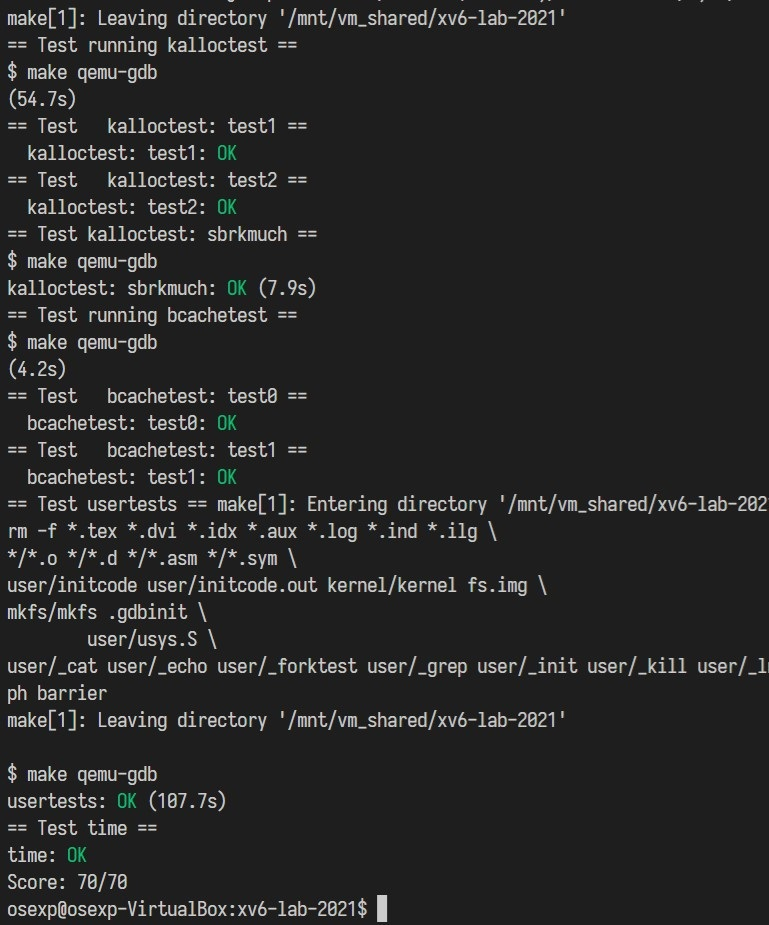
\includegraphics[width=0.5\textwidth]{lock_grade.jpg}
  \caption{ Lab Lock 的测评结果}
\end{figure}
可见测试全部通过,得分为满分。

\section{小结:减少加锁开销}

上面的两个实验很形象地展示了两种常见的减少加锁开销的方法,这里进行小结:
\begin{enumerate}
    \item 资源重复设置:在 \lstinline{kalloc} 中,通过设置多份资源以减少进程的等待概率;
    \item 细化加锁粒度:在 \lstinline{bcache} 中,通过精细化的加锁管理,减少资源加锁冲突的概率。
\end{enumerate}



\chapter{Lab File system:文件系统实验}
\begin{introduction}
    \item 使文件系统支持大文件
    \item 实现符号链接
    \item 现代的文件系统
\end{introduction}

文件系统作为操作系统的重要部分,在前面的实验中都没有涉及。因而,在本实验中,我们会深入改进 xv6 原先的文件系统,从而学习与文件系统相关的一些概念。

\section{使文件系统支持大文件}

在原始的 xv6 的实现中,其文件系统的部分与原版的 Unix v6 类似,均使用基于 inode 和目录的文件管理方式,但其 inode 仅为两级索引,共有 12 个直接索引块和 1 个间接索引块,间接索引块可以指向 256 个数据块,故而一个文件最多拥有 268 个数据块。我们需要将 xv6 的文件系统进行扩充,使之可以支持更大的文件。

xv6 的实验手册中推荐的方案是:使用三级索引,共有 11 个直接索引, 1 个间接索引块和 1 个 二级间接索引块,故总共支持文件大小为 $11 + 256 + 256 \times 256 = 65803$ 块。

首先我们修改 \lstinline{fs.h} 中的一些定义,使之符合三级索引的要求:
\begin{lstlisting}[language=C]
    #define NDIRECT 12
    #define NINDIRECT (BSIZE / sizeof(uint))
    #define MAXFILE (NDIRECT -1 + NINDIRECT + NINDIRECT * NINDIRECT)
\end{lstlisting}

由于文件的读写需要使用 \lstinline{bmap()} 来找到需要操作的文件块,故而我们修改 \lstinline{fs.c} 中用于找到文件块的 \lstinline{bmap()} ,使之能够支持三级索引。一个简单的思路是通过访问文件的位置来判断该位置是位于几级索引中,这样可以复用原先的大部分代码,而只需要实现二级间接索引的部分。笔者的实现如下:
\begin{lstlisting}[language=C]
static uint
bmap(struct inode *ip, uint bn)
{
  uint addr, *a;
  struct buf *bp;

  if(bn < NDIRECT - 1){
    if((addr = ip->addrs[bn]) == 0)
      ip->addrs[bn] = addr = balloc(ip->dev);
    return addr;
  }
  bn -= NDIRECT - 1;

  if(bn < NINDIRECT){
    // Load indirect block, allocating if necessary.
    if((addr = ip->addrs[NDIRECT - 1]) == 0)
      ip->addrs[NDIRECT - 1] = addr = balloc(ip->dev);
    bp = bread(ip->dev, addr);
    a = (uint*)bp->data;
    if((addr = a[bn]) == 0){
      a[bn] = addr = balloc(ip->dev);
      log_write(bp);
    }
    brelse(bp);
    return addr;
  }
  bn -= NINDIRECT;

  if(bn < NINDIRECT * NINDIRECT){
    uint dbr = bn / NINDIRECT;
    uint dbc = bn % NINDIRECT;
    if((addr = ip->addrs[NDIRECT]) == 0)
      ip->addrs[NDIRECT] = addr = balloc(ip->dev);
    
    bp = bread(ip->dev, addr);
    a = (uint*)bp->data;
    if((addr = a[dbr]) == 0){
      a[dbr] = addr = balloc(ip->dev);
      log_write(bp);
    }
    brelse(bp);

    bp = bread(ip->dev, addr);
    a = (uint*)bp->data;
    if((addr = a[dbc]) == 0){
      a[dbc] = addr = balloc(ip->dev);
      log_write(bp);
    }
    brelse(bp);
    return addr;
  }
  panic("bmap: out of range");
}
\end{lstlisting}

\begin{proposition}[使用 \lstinline{bmap} 的巧妙之处] 
    Unix 的文件系统中,将文件位置映射到块的位置的操作封装为 \lstinline{bmap()} 可谓十分经典的软件工程技巧。按照正常的实现思路,需要在读写函数中分别实现查找对应块的过程,而将该过程抽象出来单独处理,使得文件系统的实现更加灵活,且具有更好的可扩展性:因为若要更改文件系统的底层结构,读写的函数几乎无需更改,而只需改变文件块的查找规则即可。
\end{proposition}

此时 xv6 的文件系统应该能够支持上述的大文件,再次编译并运行 xv6 ,然后运行 \lstinline{bigfile} ,会得到类似下图的结果:
\begin{figure}[H]
  \centering
  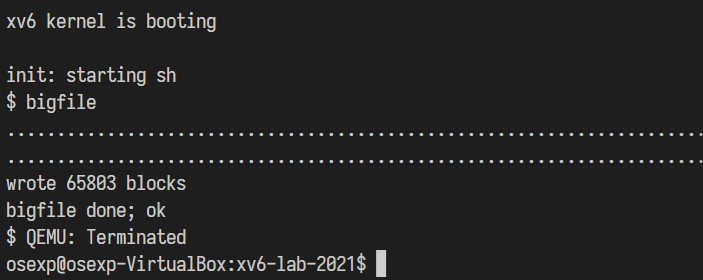
\includegraphics[width=0.8\textwidth]{fs_bigfile.jpg}
  \caption{ \lstinline{bigfile} 的测试结果}
\end{figure}

\section{实现符号链接}

在诸多类 Unix 系统中,为了方便文件管理,很多系统提供了符号链接的功能。符号链接(或软链接)是指通过路径名链接的文件; 当一个符号链接被打开时,内核会跟随链接指向被引用的文件。 符号链接类似于硬链接,但硬链接仅限于指向同一磁盘上的文件,而符号链接可以跨磁盘设备。我们需要实现一个系统调用 \lstinline{symlink(char *target, char *path)} 用于创建符号链接。

首先,按照通常的方法在 \lstinline{user/usys.pl} 和 \lstinline{user/user.h} 中加入该系统调用的入口,然后在 \lstinline{kernel/sysfile.c} 中加入空的 \lstinline{sys_symlink} 。修改头文件 \lstinline{kernel/stat.h} ,增加一个文件类型:
\begin{lstlisting}[language=C]
    #define T_SYMLINK 4   // Symbolic link
\end{lstlisting}

然后在头文件 \lstinline{kernel/fcntl.h} 加入一个标志位,供 \lstinline{open} 系统调用使用:
\begin{lstlisting}[language=C]
    #define O_NOFOLLOW  0x010
\end{lstlisting}

接着在 Makefile 中加入用户程序 \lstinline{symlinktest} ,此时应当能正常通过编译。这些准备工作完成后,我们可以真正着手实现 \lstinline{symlink(target, path)} 和对应的 \lstinline{open} 系统调用。在 \lstinline{sys_symlink} 中,仿照 \lstinline{sys_mknod} 的结构,创建节点并写入软链接的数据:
\begin{lstlisting}[language=C]
uint64 sys_symlink(void)
{
  char target[MAXPATH], path[MAXPATH];
  struct inode *ip;
  if(argstr(0, target, MAXPATH) < 0 || argstr(1, path, MAXPATH) < 0)
  {
    return -1;
  }
  begin_op();
  if((ip = namei(path)) == 0)
  {
    ip = create(path, T_SYMLINK, 0, 0);
    iunlock(ip);
  }
  ilock(ip);
  if(writei(ip, 0, (uint64)target, ip->size, MAXPATH) != MAXPATH)
  {
    return -1;
  }
  iunlockput(ip);
  end_op();
  return 0;
}
\end{lstlisting}

注意到其中调用了创建节点的函数 \lstinline{create} ,故我们也要对其进行修改:

然后修改 \lstinline{sys_open} ,使之能够跟随软链接并读取其指向的内容:
\begin{lstlisting}[language=C]
uint64
sys_open(void)
{
......
    if(ip->type == T_SYMLINK) 
    {
      if((omode & O_NOFOLLOW) == 0)
      {
        char target[MAXPATH];
        int recursive_depth = 0;
        while(1)
        {
          if(recursive_depth >= 10)
          {
	        iunlockput(ip);
	        end_op();
	        return -1;
	      }
          if(readi(ip, 0, (uint64)target, ip->size-MAXPATH, MAXPATH) != MAXPATH)
          {
	        return -1;
	      }
          iunlockput(ip);
	      if((ip = namei(target)) == 0)
          {
	        end_op();
	        return -1;
	      }
	      ilock(ip);
	      if(ip->type != T_SYMLINK)
          {
	      break;
	      }
	      recursive_depth++;
        }
      }
    }
......
\end{lstlisting}

至此,对于 xv6 的软链接功能已经完成,再次编译并运行 xv6 ,然后运行 \lstinline{symlinktest} ,会得到类似下图的结果:
\begin{figure}[H]
  \centering
  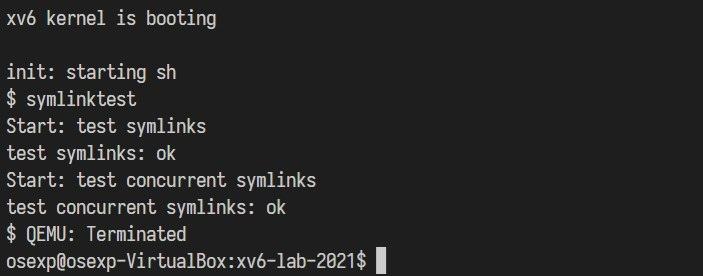
\includegraphics[width=0.8\textwidth]{fs_symlink.jpg}
  \caption{ \lstinline{symlinktest} 的测试结果}
\end{figure}

可见成功通过测试。

\paragraph*{实验结果} 在完成 Lab File system 中的所有实验后,根据 MIT 6.S081 的传统,需要在实验目录下创建一个名为 \lstinline{time.txt} 文本文件,其中只包含一行,为完成该实验的小时数。然后在终端中执行 \lstinline{make grade} ,即可对整个实验进行自动评分,笔者的结果如下:
\begin{figure}[H]
  \centering
  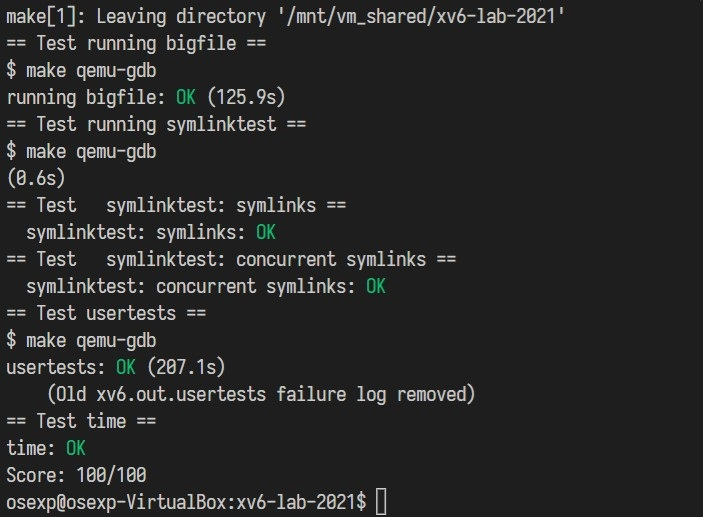
\includegraphics[width=0.8\textwidth]{fs_grade.jpg}
  \caption{ Lab File system 的测评结果}
\end{figure}

可见测试全部通过,得分为满分。

\begin{theorem}[注意 inode 加锁及其不同形态]
    在实现软链接的过程中,我们会碰到很多直接操作 inode 的情况。这些操作分布在不同的源文件中,有着复杂的加锁和写回机制,并且有着严格的执行条件。为了理清这些操作,需要理解 inode 、 inode 在内存中的映像和物理块等概念,并且仔细阅读各个函数前的说明:它们会提示我们该函数对目前加锁情况的要求,以及在函数完成后加锁情况的变化。
\end{theorem}
\section{小结:现代的文件系统}

在这个实验中,我们已经涉及了 Unix 文件系统的很多特性,且被我们完善过的 xv6 文件系统已经与一些较早的现代文件系统(如 ext2 )几乎一致,包括了如下的特性:
\begin{enumerate}
    \item 基于 inode 的多级索引文件组织
    \item 日志文件系统
    \item 硬链接和软链接
    \item inode 缓存与数据块缓存
    \item 基于缓存的写入优化
\end{enumerate}

但是,在上面的实验中,仍有一些现代文件系统的特性在 xv6 中没有被涉及,这里小结如下:
\begin{enumerate}
    \item 基于 Extent 的空间管理方式
    \item 成组的空间管理
    \item 基于 B 树的索引
    \item 原子性读写操作
    \item 跨物理卷管理
    \item 软件 Raid 机制
    \item 快照机制
    \item 只读文件系统优化
\end{enumerate}

上面一些机制在目前的一些文件系统中有着广泛的应用,就笔者的个人观点,参考学习 ext4 、 xfs 、 btrfs 、 erofs 这几个极具代表性的现代文件系统,便可以对上述特性的原理与实现有所了解,并且把握操作系统中文件系统的发展方向。
\chapter{Lab mmap:内存映射实验}
\begin{introduction}
    \item 实现 mmap 内存映射系统调用
    \item 再次俯瞰 xv6
\end{introduction}

虽然在现代的 Linux 操作系统中,由于新的机制的引入, mmap 系统调用已经成为 glibc 在很多情形下的备选方案,但这并不影响 mmap 作为经典的 Unix 系统调用的地位。为 xv6 实现 mmap 的过程会涉及修改操作系统的几乎每个部分,故而作为压轴实验供我们把玩。

\section{实现 mmap 内存映射系统调用}

真正的 mmap 为用户程序提供了精细化操作它们地址空间的手段,包括但不限于:共享进程间的地址空间,将文件映射到地址空间,用户处理缺页错误等功能。我们需要为 xv6 添加的 mmap 只需要实现将文件映射到地址空间的功能,其接受的参数如下:
\begin{lstlisting}[language=C]
void *mmap(void *addr, size_t length, int prot, int flags,
    int fd, off_t offset);
\end{lstlisting}

此外,另有一个用于取消 mmap 映射的系统调用 \lstinline{munmap(addr, length)} ,除了移除映射外,其根据实际情况可能需要将映射的文件写回。

xv6 实验和往常一样,为我们提供了用户态测评程序 \lstinline{mmaptest} 。在该测评程序中, addr 和 offset 总是为 0 ,意味着内核可以自由选择映射的地址,并总是从文件开头开始映射;若映射失败,则返回 \lstinline{0xffffffffffffffff} 。我们只需实现 \lstinline{mmaptest} 中用到的功能。

首先照例在 Makefile 中添加用户态测评程序 \lstinline{mmaptest} ,然后添加空的 \lstinline{mmap} 和 \lstinline{munmap} ,使得编译通过:
\begin{lstlisting}[language=C]
    Makefile:
    ==============================
    UPROGS=\
    ......
    	$U/_mmaptest\
    ......
    ==============================
    
    kernel/syscall.h
    ==============================
    ......
    #define SYS_mmap   22
    #define SYS_munmap 23
    ==============================
    
    kernel/syscall.c
    ==============================
    ......
    extern uint64 sys_mmap(void);
    extern uint64 sys_munmap(void);
    ......
    static uint64 (*syscalls[])(void) = {
    ......
    [SYS_mmap]    sys_mmap,
    [SYS_munmap]  sys_munmap,
    };
    ......
    ==============================
    
    kernel/sysproc.c
    ==============================
    ......
    void *sys_mmap(void)
    {
      return (void *)-1;
    }
    
    int sys_munmap(void)
    {
      return -1;
    }
    ......
    ==============================
    
    user/user.h
    ==============================
    ......
    void *mmap(void *, int, int, int, int, int);
    int munmap(void *, int);
    ......
    ==============================
    
    user/usys.pl
    ==============================
    ......
    entry("mmap");
    entry("munmap");
    ......
    ==============================
\end{lstlisting}

此时执行 \lstinline{make} ,应当能够编译通过。按照 xv6 实验手册的提示,在 \lstinline{proc.h} 中加入 VMA 数据结构的定义,并给进程控制块中加入 VMA 指针:
\begin{lstlisting}[language=C]
#define NVMA 16
#define VMA_START (MAXVA >> 1)

struct vma {
  uint64 start;
  uint64 end;
  uint64 length; // 0 -> not used
  uint64 off;

  int perm;
  int flags;
  struct file *file;
  struct vma *next;

  struct spinlock lock;
};

// Per-process state
struct proc {
......
  struct vma *vma;             // VMA item
};
\end{lstlisting}

为了避免于堆和栈冲突,这里我们决定将内存映射开始于最大地址的一半处。由于后续需要多次对 VMA 进行分配,故而将其封装为一个函数会更加方便,\lstinline{proc.c} 中加入:
\begin{lstlisting}[language=C]
......
// VMA list
struct vma vma_list[NVMA];

struct vma* vma_alloc() 
{
  for(int i = 0; i < NVMA; i++)
  {
    acquire(&vma_list[i].lock);
    if (vma_list[i].length == 0)
    {
      return &vma_list[i];
    } else 
    {
      release(&vma_list[i].lock);
    }
  }
  panic("no free vma");
}
......
\end{lstlisting}

然后,根据实验手册的提示,我们无需真正在 \lstinline{sys_mmap} 中完成内存映射,而是通过一个惰性机制,在出现缺页异常时再进行映射,故而我们在 \lstinline{sys_mmap} 中只需完成对 VMA 的设置:
\begin{lstlisting}[language=C]
#include "types.h"
#include "param.h"
#include "date.h"
#include "spinlock.h"
#include "sleeplock.h"
#include "fs.h"
#include "memlayout.h"
#include "riscv.h"
#include "defs.h"
#include "proc.h"
#include "fcntl.h"
#include "file.h"
......
extern struct vma *vma_alloc();
void *sys_mmap(void)
{
  uint64 addr;
  struct proc *p = myproc();
  int length, prot, flags, fd, offset;

  if (argaddr(0, &addr) < 0)
    return (void *)-1;
  if (argint(1, &length) < 0)
    return (void *)-1;
  if (argint(2, &prot) < 0)
    return (void *)-1;
  if (argint(3, &flags) < 0)
    return (void *)-1;
  if (argint(4, &fd) < 0)
    return (void *)-1;
  if (argint(5, &offset) < 0)
    return (void *)-1;
  if (addr != 0)
    addr = 0;
  if (offset != 0)
    offset = 0;

  struct file *f = p->ofile[fd];

  // Check flags
  int pte_flag = PTE_U;
  if (prot & PROT_READ)
  {
    if (!f->readable)
      return (void *)-1;
    pte_flag |= PTE_R;
  }
  if (prot & PROT_WRITE)
  {
    if (!f->writable && !(flags & MAP_PRIVATE))
      return (void *)-1;
    pte_flag |= PTE_W;
  }

  // Setting up vma
  struct vma *v = vma_alloc();
  v->perm = pte_flag;
  v->length = length;
  v->off = offset;
  v->file = myproc()->ofile[fd];
  v->flags = flags;
  filedup(f);
  struct vma *pv = p->vma;
  if (pv == 0)
  {
    v->start = VMA_START;
    v->end = length + v->start;
    p->vma = v;
  }
  else
  {
    while (pv->next)
      pv = pv->next;
    v->start = PGROUNDUP(pv->end);
    v->end = v->start + length;
    pv->next = v;
    v->next = 0;
  }
  addr = v->start;
  release(&v->lock);
  return (void *)(addr);
}
......
\end{lstlisting}

为了在 \lstinline{usertrap} 中处理 mmap 造成的缺页异常,我们首先编写相关的中断处理过程 \lstinline{mmap_alloc} :
\begin{lstlisting}[language=C]
#include "types.h"
#include "param.h"
#include "memlayout.h"
#include "riscv.h"
#include "spinlock.h"
#include "sleeplock.h"
#include "proc.h"
#include "defs.h"
#include "fs.h"
#include "file.h"
......
int mmap_alloc(uint64 va, int scause)
{
  struct proc *p = myproc();
  struct vma* v = p->vma;

  while(v != 0)
  {
    if (va >= v->start && va < v->end)
    {
      break;
    }
    v = v->next;
  }

  if (v == 0) 
    return -1; 
  if (scause == 13 && !(v->perm & PTE_R)) 
    return -1; 
  if (scause == 15 && !(v->perm & PTE_W)) 
    return -1;
  
  // load from file
  va = PGROUNDDOWN(va);
  char* mmem = kalloc();
  if (mmem == 0) 
    return -1;
  memset(mmem, 0, PGSIZE);

  if (mappages(p->pagetable, va, PGSIZE, (uint64)mmem, v->perm) != 0)
  {
    kfree(mmem);
    return -1;
  }

  struct file *f = v->file;
  ilock(f->ip);
  readi(f->ip, 0, (uint64)mmem, v->off + va - v->start, PGSIZE);
  iunlock(f->ip);
  return 0;
}
......
\end{lstlisting}

在 \lstinline{usertrap} 中调用 \lstinline{mmap_alloc} :
\begin{lstlisting}[language=C]
void
usertrap(void)
{
......
  } else if((r_scause() == 13) || (r_scause() == 15)){  // page fault
    if (mmap_alloc(r_stval(), r_scause()) != 0) 
    {
      printf("mmap: page fault\n");
      p->killed = 1;
    }
  } else {

}
\end{lstlisting}

此时, mmap 的前半部分基本完成,接下来需要实现 \lstinline{munmap} 。思路与之前类似,除了操作 VMA 外,一个难点在于写回。为此我们先实现写回的函数:
\begin{lstlisting}[language=C]
void write_back(struct vma *v, uint64 addr, int n)
{
  // no need to writeback
  if (!(v->perm & PTE_W) || (v->flags & MAP_PRIVATE))
    return;
  if ((addr % PGSIZE) != 0)
    panic("unmap: not aligned");
  struct file *f = v->file;
  int max = ((MAXOPBLOCKS - 1 - 1 - 2) / 2) * BSIZE;
  int i = 0;
  while (i < n)
  {
    int k = n - i;
    if (k > max)
      k = max;
    begin_op();
    ilock(f->ip);
    int wcnt = writei(f->ip, 1, addr + i, v->off + v->start - addr + i, k);
    iunlock(f->ip);
    end_op();
    i += wcnt;
  }
}
\end{lstlisting}

然后实现 \lstinline{sys_munmap} ,根据 xv6 的要求,只需分在头尾释放两种不同的情况,中间释放的部分无需考虑:
\begin{lstlisting}[language=C]
int sys_munmap(void)
{
  uint64 addr;
  int length;
  if (argaddr(0, &addr) < 0)
    return -1;
  if (argint(1, &length) < 0)
    return -1;
  struct proc *p = myproc();
  struct vma *v = p->vma;
  struct vma *pre = 0;
  while (v != 0)
  {
    if (addr >= v->start && addr < v->end)
      break;
    pre = v;
    v = v->next;
  }
  // not mapped
  if (v == 0)
    return -1;
  if (addr != v->start && addr + length != v->end)
    panic("munmap: middle of vma");
  if (addr == v->start)
  {
    write_back(v, addr, length);
    uvmunmap(p->pagetable, addr, length / PGSIZE, 1);
    if (length == v->length)
    {
      // free all
      fileclose(v->file);
      if (pre == 0)
      {
        p->vma = v->next;
      }
      else
      {
        pre->next = v->next;
        v->next = 0;
      }
      acquire(&v->lock);
      v->length = 0;
      release(&v->lock);
    }
    else
    {
      // head
      v->start -= length;
      v->off += length;
      v->length -= length;
    }
  }
  else
  {
    // tail
    v->length -= length;
    v->end -= length;
  }
  return 0;
}
\end{lstlisting}

至此, mmap 整体上就算完成了,但是仍有两个细节需要注意:一是 fork 时需要将父进程的 VMA 复制给子进程,二是进程退出时也需要写回所有内容。首先处理 fork :
\begin{lstlisting}[language=C]
int fork(void)
{
......
  acquire(&np->lock);
  np->state = RUNNABLE;
  np->vma = 0;
  struct vma *pvma = p->vma;
  struct vma *pre = 0;
  while (pvma)
  {
    struct vma *nvma = vma_alloc();
    nvma->start = pvma->start;
    nvma->end = pvma->end;
    nvma->off = pvma->off;
    nvma->length = pvma->length;
    nvma->perm = pvma->perm;
    nvma->flags = pvma->flags;
    nvma->file = pvma->file;
    filedup(nvma->file);
    nvma->next = 0;
    if (pre == 0)
    {
      np->vma = nvma;
    }
    else
    {
      pre->next = nvma;
    }
    pre = nvma;
    release(&nvma->lock);
    pvma = pvma->next;
  }
  release(&np->lock);

  return pid;
}
\end{lstlisting}

再处理 exit 系统调用:
\begin{lstlisting}[language=C]
extern void write_back(struct vma *v, uint64 addr, int n);
void exit(int status)
{
  struct proc *p = myproc();

  if (p == initproc)
    panic("init exiting");

  // mUnmap all vma
  struct vma *v = p->vma;
  struct vma *pvma;
  while (v)
  {
    write_back(v, v->start, v->length);
    uvmunmap(p->pagetable, v->start, PGROUNDUP(v->length) / PGSIZE, 1);
    fileclose(v->file);
    pvma = v->next;
    acquire(&v->lock);
    v->next = 0;
    v->length = 0;
    release(&v->lock);
    v = pvma;
  }

  // Close all open files.
......
}
\end{lstlisting}

至此, munmap 部分大致完成。编译并运行 xv6 ,然后运行 \lstinline{mmaptest} ,会基本通过测试,但最后一项中会得到 \lstinline{panic: uvmunmap: walk} 错误。由于 mmap 机制与原有页表的标志位含义有冲突,故此时需修改 \lstinline{vm.c} ,进行如下修改:
\begin{lstlisting}[language=C]
void
uvmunmap(pagetable_t pagetable, uint64 va, uint64 npages, int do_free)
{
  uint64 a;
  pte_t *pte;

  if((va % PGSIZE) != 0)
    panic("uvmunmap: not aligned");

  for(a = va; a < va + npages*PGSIZE; a += PGSIZE){
    if((pte = walk(pagetable, a, 0)) == 0)
      // panic("uvmunmap: walk");
      continue;
    if((*pte & PTE_V) == 0)
      // panic("uvmunmap: not mapped");
      continue;
    if(PTE_FLAGS(*pte) == PTE_V)
      panic("uvmunmap: not a leaf");
    if(do_free){
      uint64 pa = PTE2PA(*pte);
      kfree((void*)pa);
    }
    *pte = 0;
  }
}
......
void
freewalk(pagetable_t pagetable)
{
  // there are 2^9 = 512 PTEs in a page table.
  for(int i = 0; i < 512; i++){
    pte_t pte = pagetable[i];
    if((pte & PTE_V) && (pte & (PTE_R|PTE_W|PTE_X)) == 0){
      // this PTE points to a lower-level page table.
      uint64 child = PTE2PA(pte);
      freewalk((pagetable_t)child);
      pagetable[i] = 0;
    } else if(pte & PTE_V){
      // panic("freewalk: leaf");
      continue;
    }
  }
  kfree((void*)pagetable);
}
\end{lstlisting}

\begin{theorem}[为何此处忽视 panic]
    由于前文 mmap 映射的页的标志位会导致原先判断 panic 的条件被触发,从而使得在 fork 或 exit 时复制或释放页面时出现预期外的 panic ,故而此处将 panic 的语句均换为继续执行。
\end{theorem}

编译并运行 xv6 ,然后运行 \lstinline{mmaptest} ,得到类似下图的结果:
\begin{figure}[H]
  \centering
  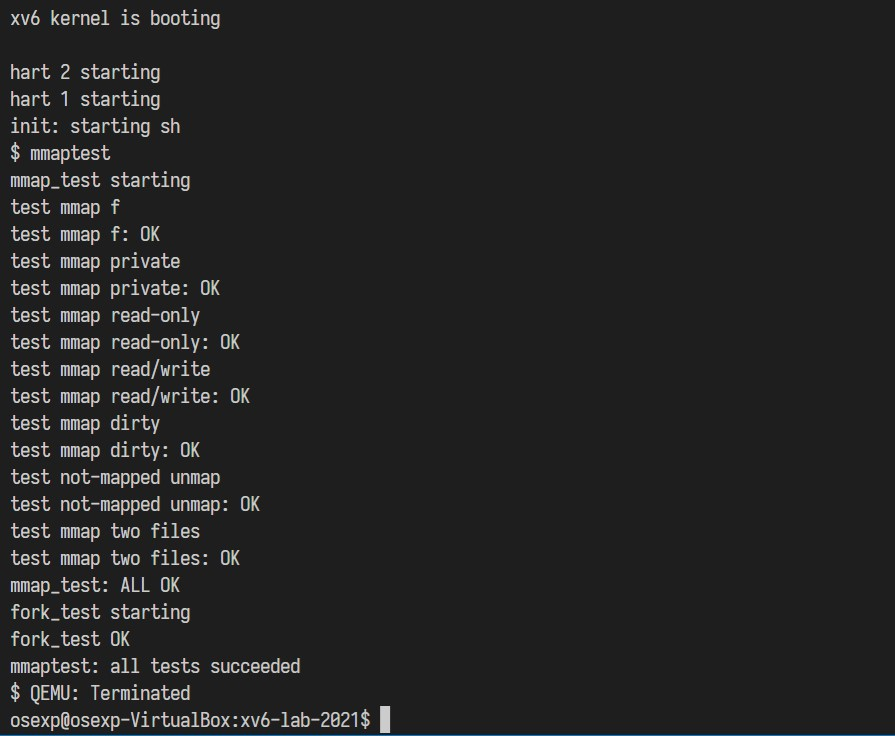
\includegraphics[width=0.6\textwidth]{mmap_mmaptest.jpg}
  \caption{ \lstinline{mmaptest} 的测试结果}
\end{figure}

测试成功通过。

\paragraph*{实验结果} 在完成 Lab mmap 中的所有实验后,根据 MIT 6.S081 的传统,需要在实验目录下创建一个名为 \lstinline{time.txt} 文本文件,其中只包含一行,为完成该实验的小时数。然后在终端中执行 \lstinline{make grade} ,即可对整个实验进行自动评分,笔者的结果如下:
\begin{figure}[H]
  \centering
  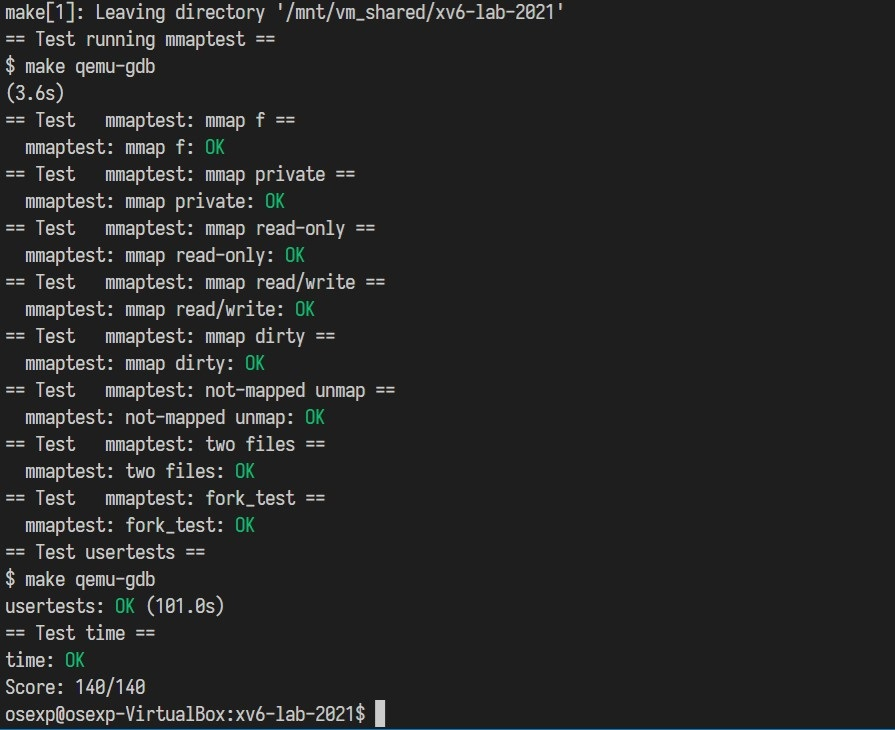
\includegraphics[width=0.6\textwidth]{mmap_grade.jpg}
  \caption{ Lab mmap 的测评结果}
\end{figure}

可见测试全部通过,得分为满分。

\section{小结:再次俯瞰 xv6}

在 mmap 实验中,我们用到了 xv6 提供的大部分机制,以它们为基础实现了较为复杂的功能。该实验作为 6.S081 提供的实验手册中的最后一次实验,起到了很好的总结作用,这里笔者也对整个 xv6 的结构做一个小结。

从用户侧来看,用户使用的主要是 \lstinline{user/user.h} ,其中包含系统调用的接口和一个 C 函数库提供的函数。系统调用接口的实现是在 \lstinline{user/usys.S} 中,而用户 C 函数库则是在 \lstinline{user/ulib.c} 中实现的。

\begin{figure}[H]
  \centering
  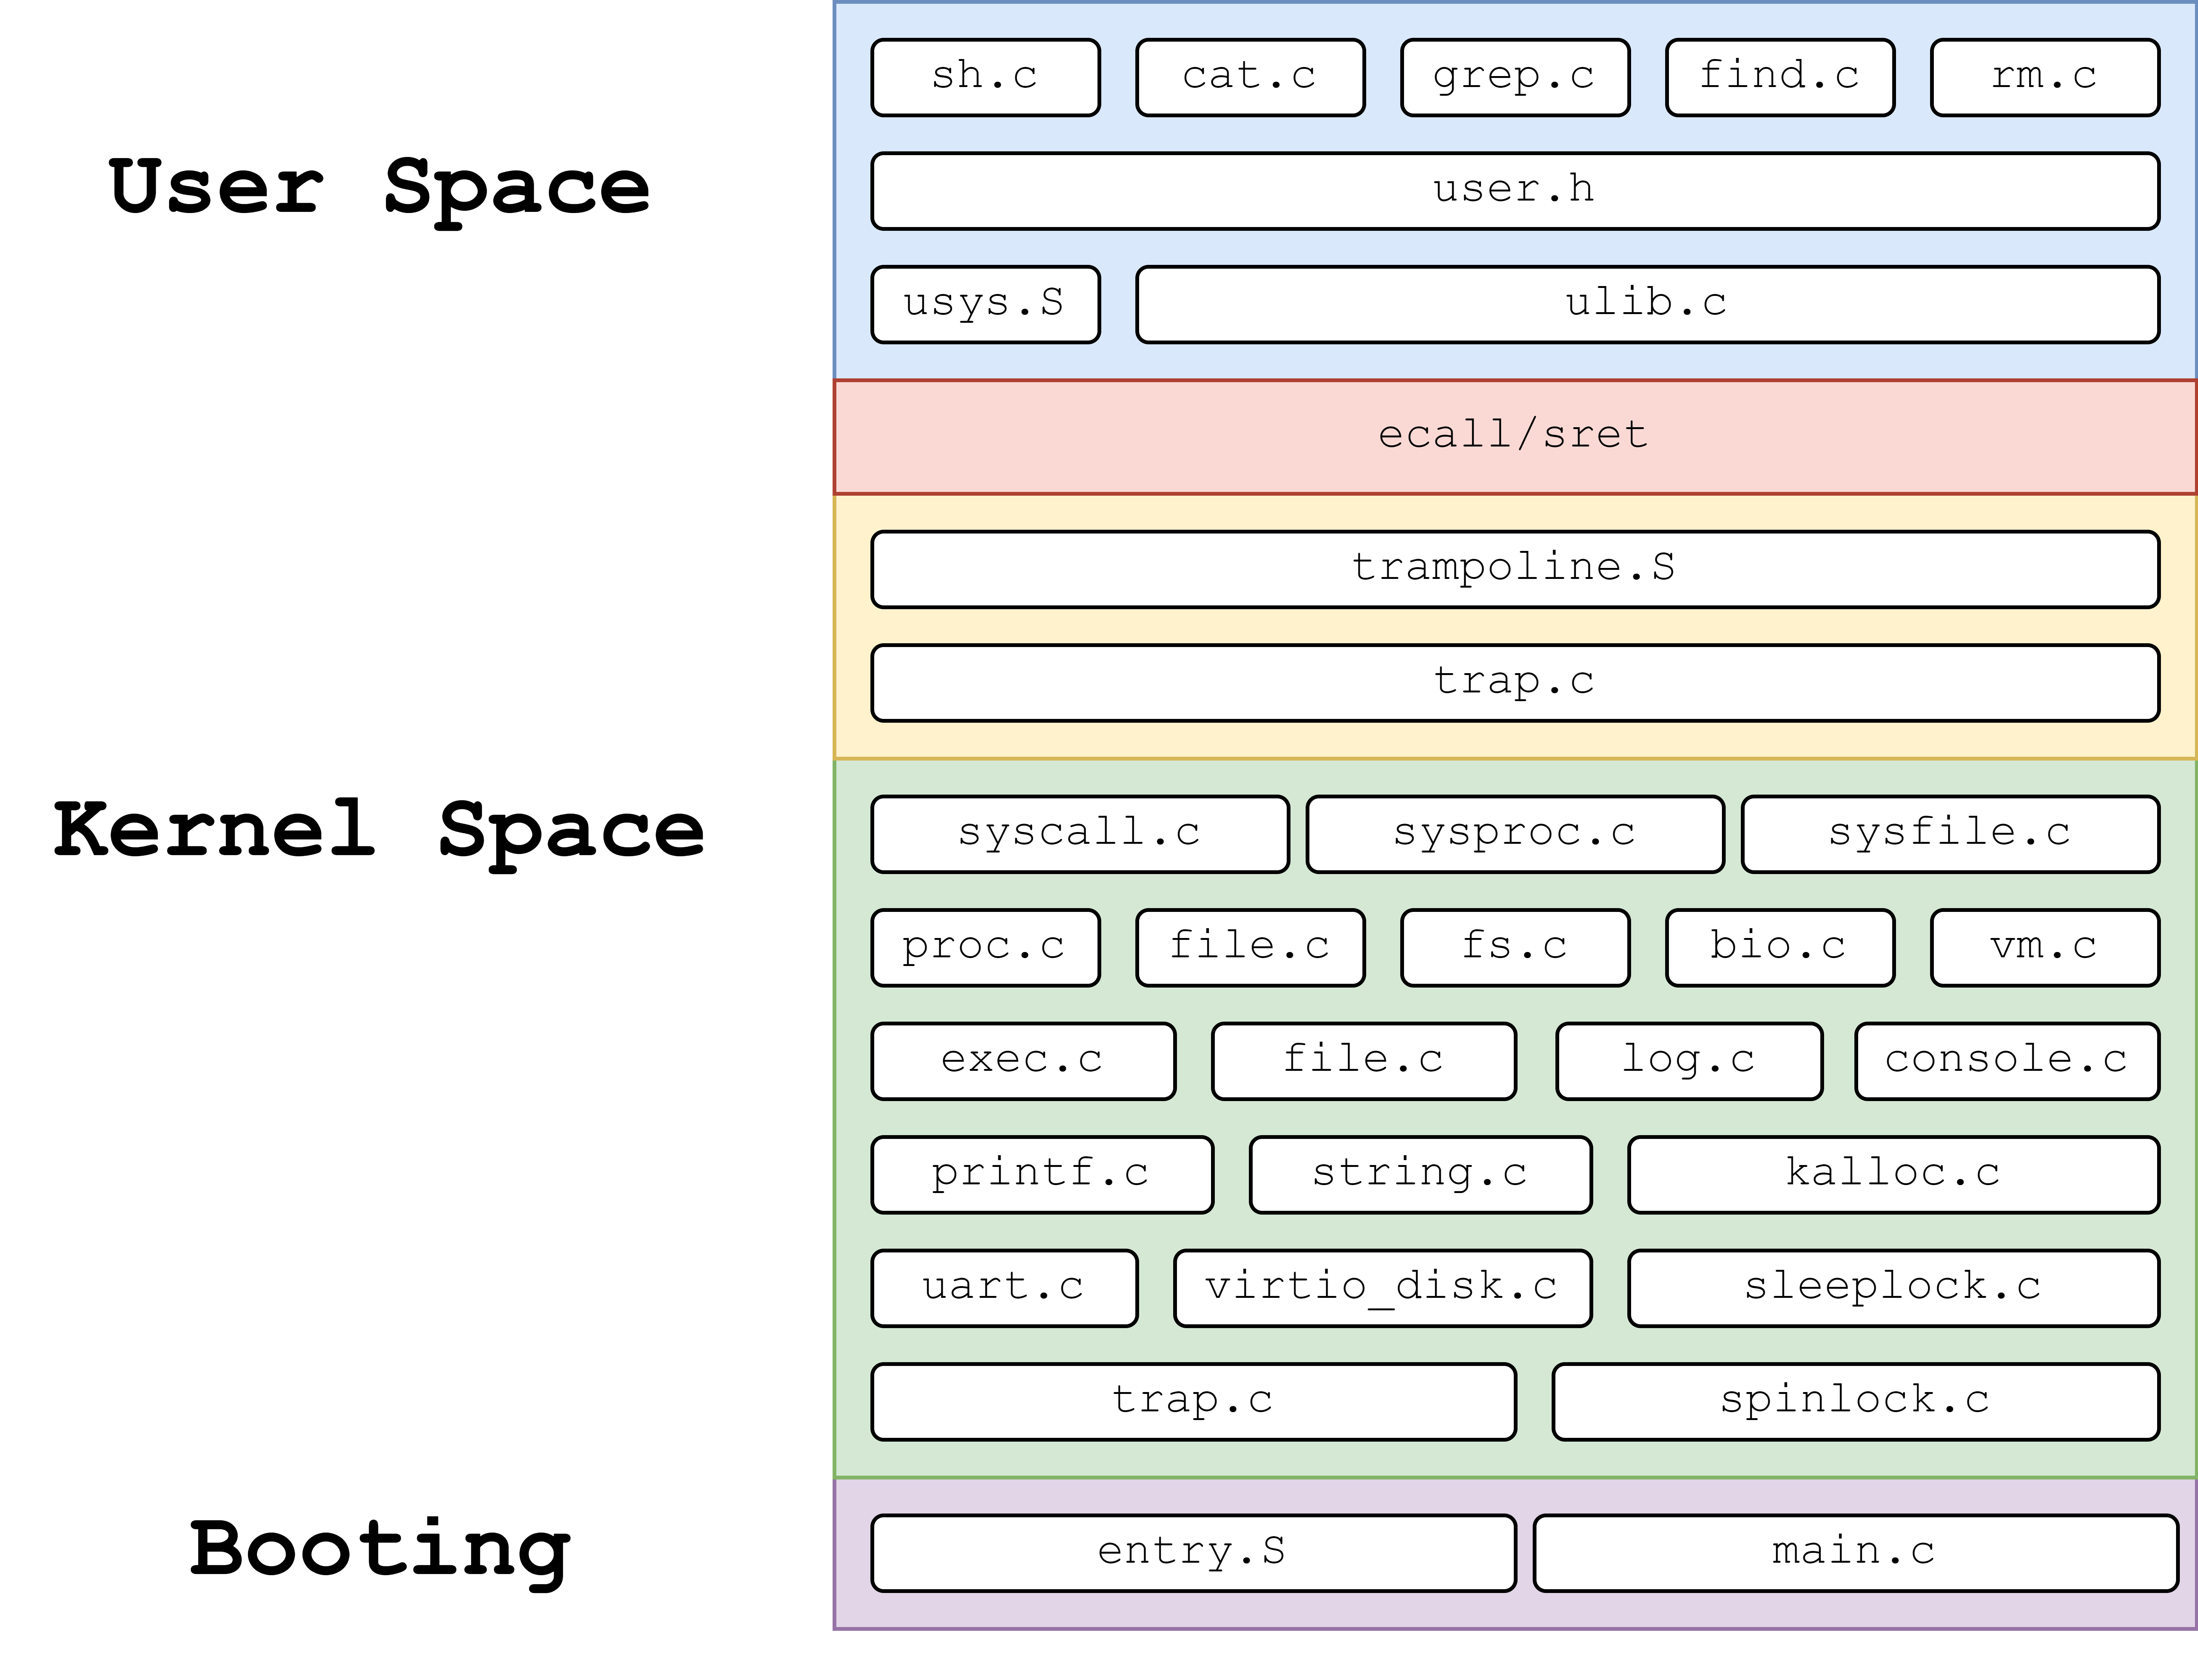
\includegraphics[width=0.8\textwidth]{xv6_arch.drawio.png}
  \caption{ xv6 结构概览 }
\end{figure}

通过 RISC-V 提供的特权指令,结合 \lstinline{trampoline.S} ,则可以完成从用户侧到内核态的跳跃; Trampoline 一词意为“蹦床”,十分形象得描述了这个过程。完成了用户侧到内核态的上下文保存与切换后,控制权移交给了 \lstinline{kernel/trap.c} 用于处理中断。内核中的诸多源文件实现了各类服务,虽然 xv6 是宏内核,但其中也有层次之分,一些较为靠近底层的功能实现和较靠近用户侧的实现是归入不同的源码文件中的:在上图中,越靠下的部分越接近硬件,诸如 \lstinline{uart.c} 等,是用于为内核中函数提供基本功能的驱动程序。还有一部分代码用于系统的初始化,这部分代码会负责从 M 态到 S 态的设置,并且为中断机制、内核内存布局进行初始化。

现代操作系统虽然也大致为分层的偏向宏内核的架构,但由于存在内核模块等机制,使得操作系统能够在运行时动态得加载或卸载功能,大大增加了操作系统的灵活性与可维护性。
\chapter{实验做好之后...}
\begin{introduction}
    \item 把 xv6 跑在国产硬件上
    \item 给 xv6 增加一个应用编程语言
    \item 更多好玩的计划
\end{introduction}

完成了全部的 xv6 实验后, xv6 作为现代体系结构上对 Unix v6 的一次复刻,其可玩性不只于 6.S081 提供的实验题目。下面笔者进行了两个额外的有趣的关于 xv6-riscv 的实验,供读者参考。

\section{把 xv6 跑在国产硬件上}

\subsection{Lichee RV 开发板概览}

虽然 RISC-V 架构仍然没有成熟的商业产品,但我国仍然有一些公司致力于开拓计算机系统结构的最新领域,并且产出了很好的成品。

今年年初,有一款国产 RISC-V 开发版凭借其极其低廉的价格迅速占据了市场,即 Lichee RV - Nezha CM \footnote{Lichee RV - Nezha CM \url{https://wiki.sipeed.com/hardware/zh/lichee/RV/RV.html}} 。该开发板使用的CPU是全志D1,其是一块基于阿里平头哥玄铁 C906 IP核的微处理器,兼容 RISC-V 的 RV64IMAC 指令集,拥有 512MB 的 DDR3 内存,并有可用的 MMU 提供对操作系统的支持。该开发板 CPU 的功能如下图所示:

\begin{figure}[H]
  \centering
  \includegraphics[width=0.5\textwidth]{c906.png}
  \caption{ C906 结构概览 }
\end{figure}

关于 C906 的文档可以在阿里平头哥的GitHub库里找到\footnote{参见:\url{https://github.com/T-head-Semi/openc906/tree/main/doc}},但对于 Lichee RV 开发板,由于一些商业上知识产权的原因,该开发板的很多外设的驱动都是不公开的;但幸运的是,运行 xv6 所需要的 uart 驱动是可用的,故而笔者在查阅了众多资料后,自费入手了一块 Lichee RV ,企图将 xv6 移植到其上并成功通过 \lstinline{usertests} 。

笔者购得的 Lichee RV 如下图所示:

\begin{figure}[H]
  \centering
  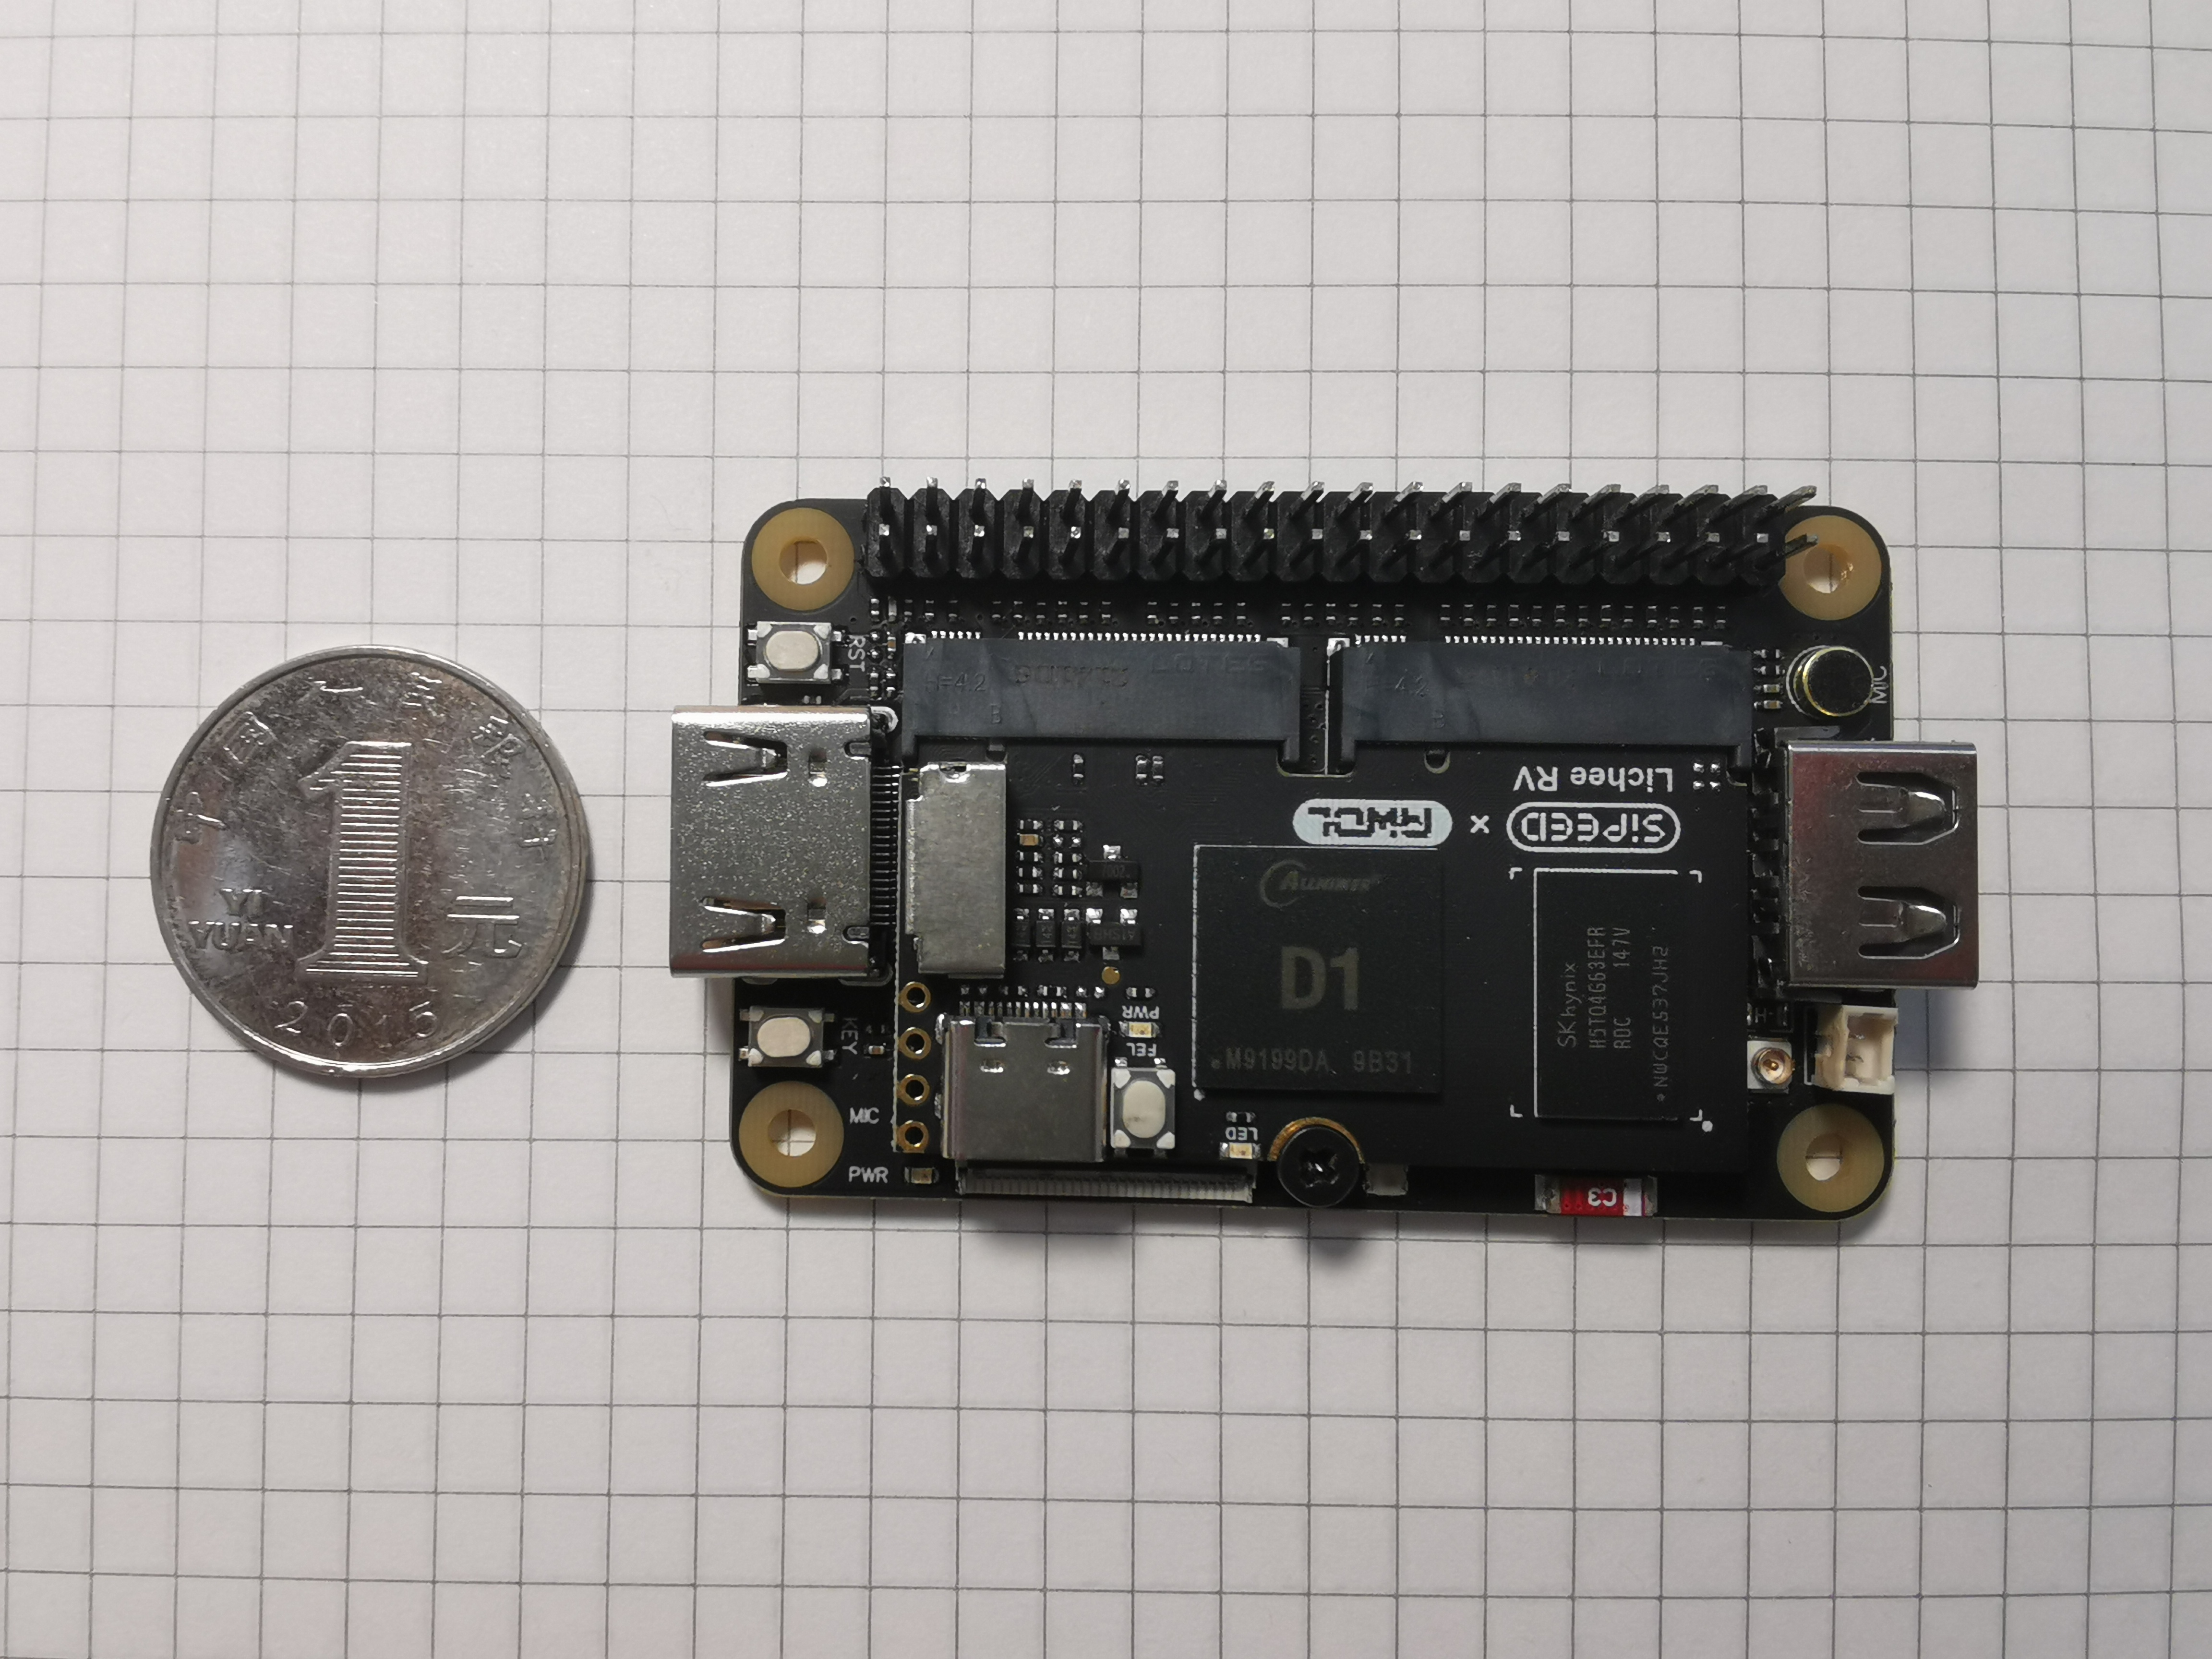
\includegraphics[width=0.7\textwidth]{LC_RV.jpg}
  \caption{ 笔者的 Lichee RV 开发板 }
\end{figure}

\subsection{前期准备}

在开始移植前,我们需要准备一份干净的 xv6-riscv 代码库,在终端中执行 \lstinline{git clone git://github.com/mit-pdos/xv6-riscv.git} 将代码库克隆到本地。

然后,我们需要从GitHub上下载用于调试开发板的工具 \lstinline{xfel} \footnote{\url{https://github.com/xboot/xfel}} 用于将我们移植好的 xv6 内核加载到开发板内存中并开始执行。之后需要准备串口通信软件,笔者使用的是 Putty。

\begin{theorem}[在 Windows 系统上使用 \lstinline{xfel}]
    在 Windows 系统上使用 \lstinline{xfel} 还需要安装 \lstinline{zadig-2.7.exe} 驱动,才能正常使用。Windows 平台驱动和预编译的 \lstinline{xfel} 程序可以在 \url{https://github.com/xboot/xfel/releases/download/v1.2.9/xfel-windows-v1.2.9.7z} 下载。
\end{theorem}

除了软件和开发板以外。我们还需要准备一根 USB C-type 线用于通过 \lstinline{xfel} 刷写开发板,以及一块诸如 CH341 的 USB 转串口的设备,用于通过 uart 与开发板进行通信。当然,几根杜邦线也是必不可少的,(除了一台PC机外)全部需要用到的设备如下图所示:

\begin{figure}[H]
  \centering
  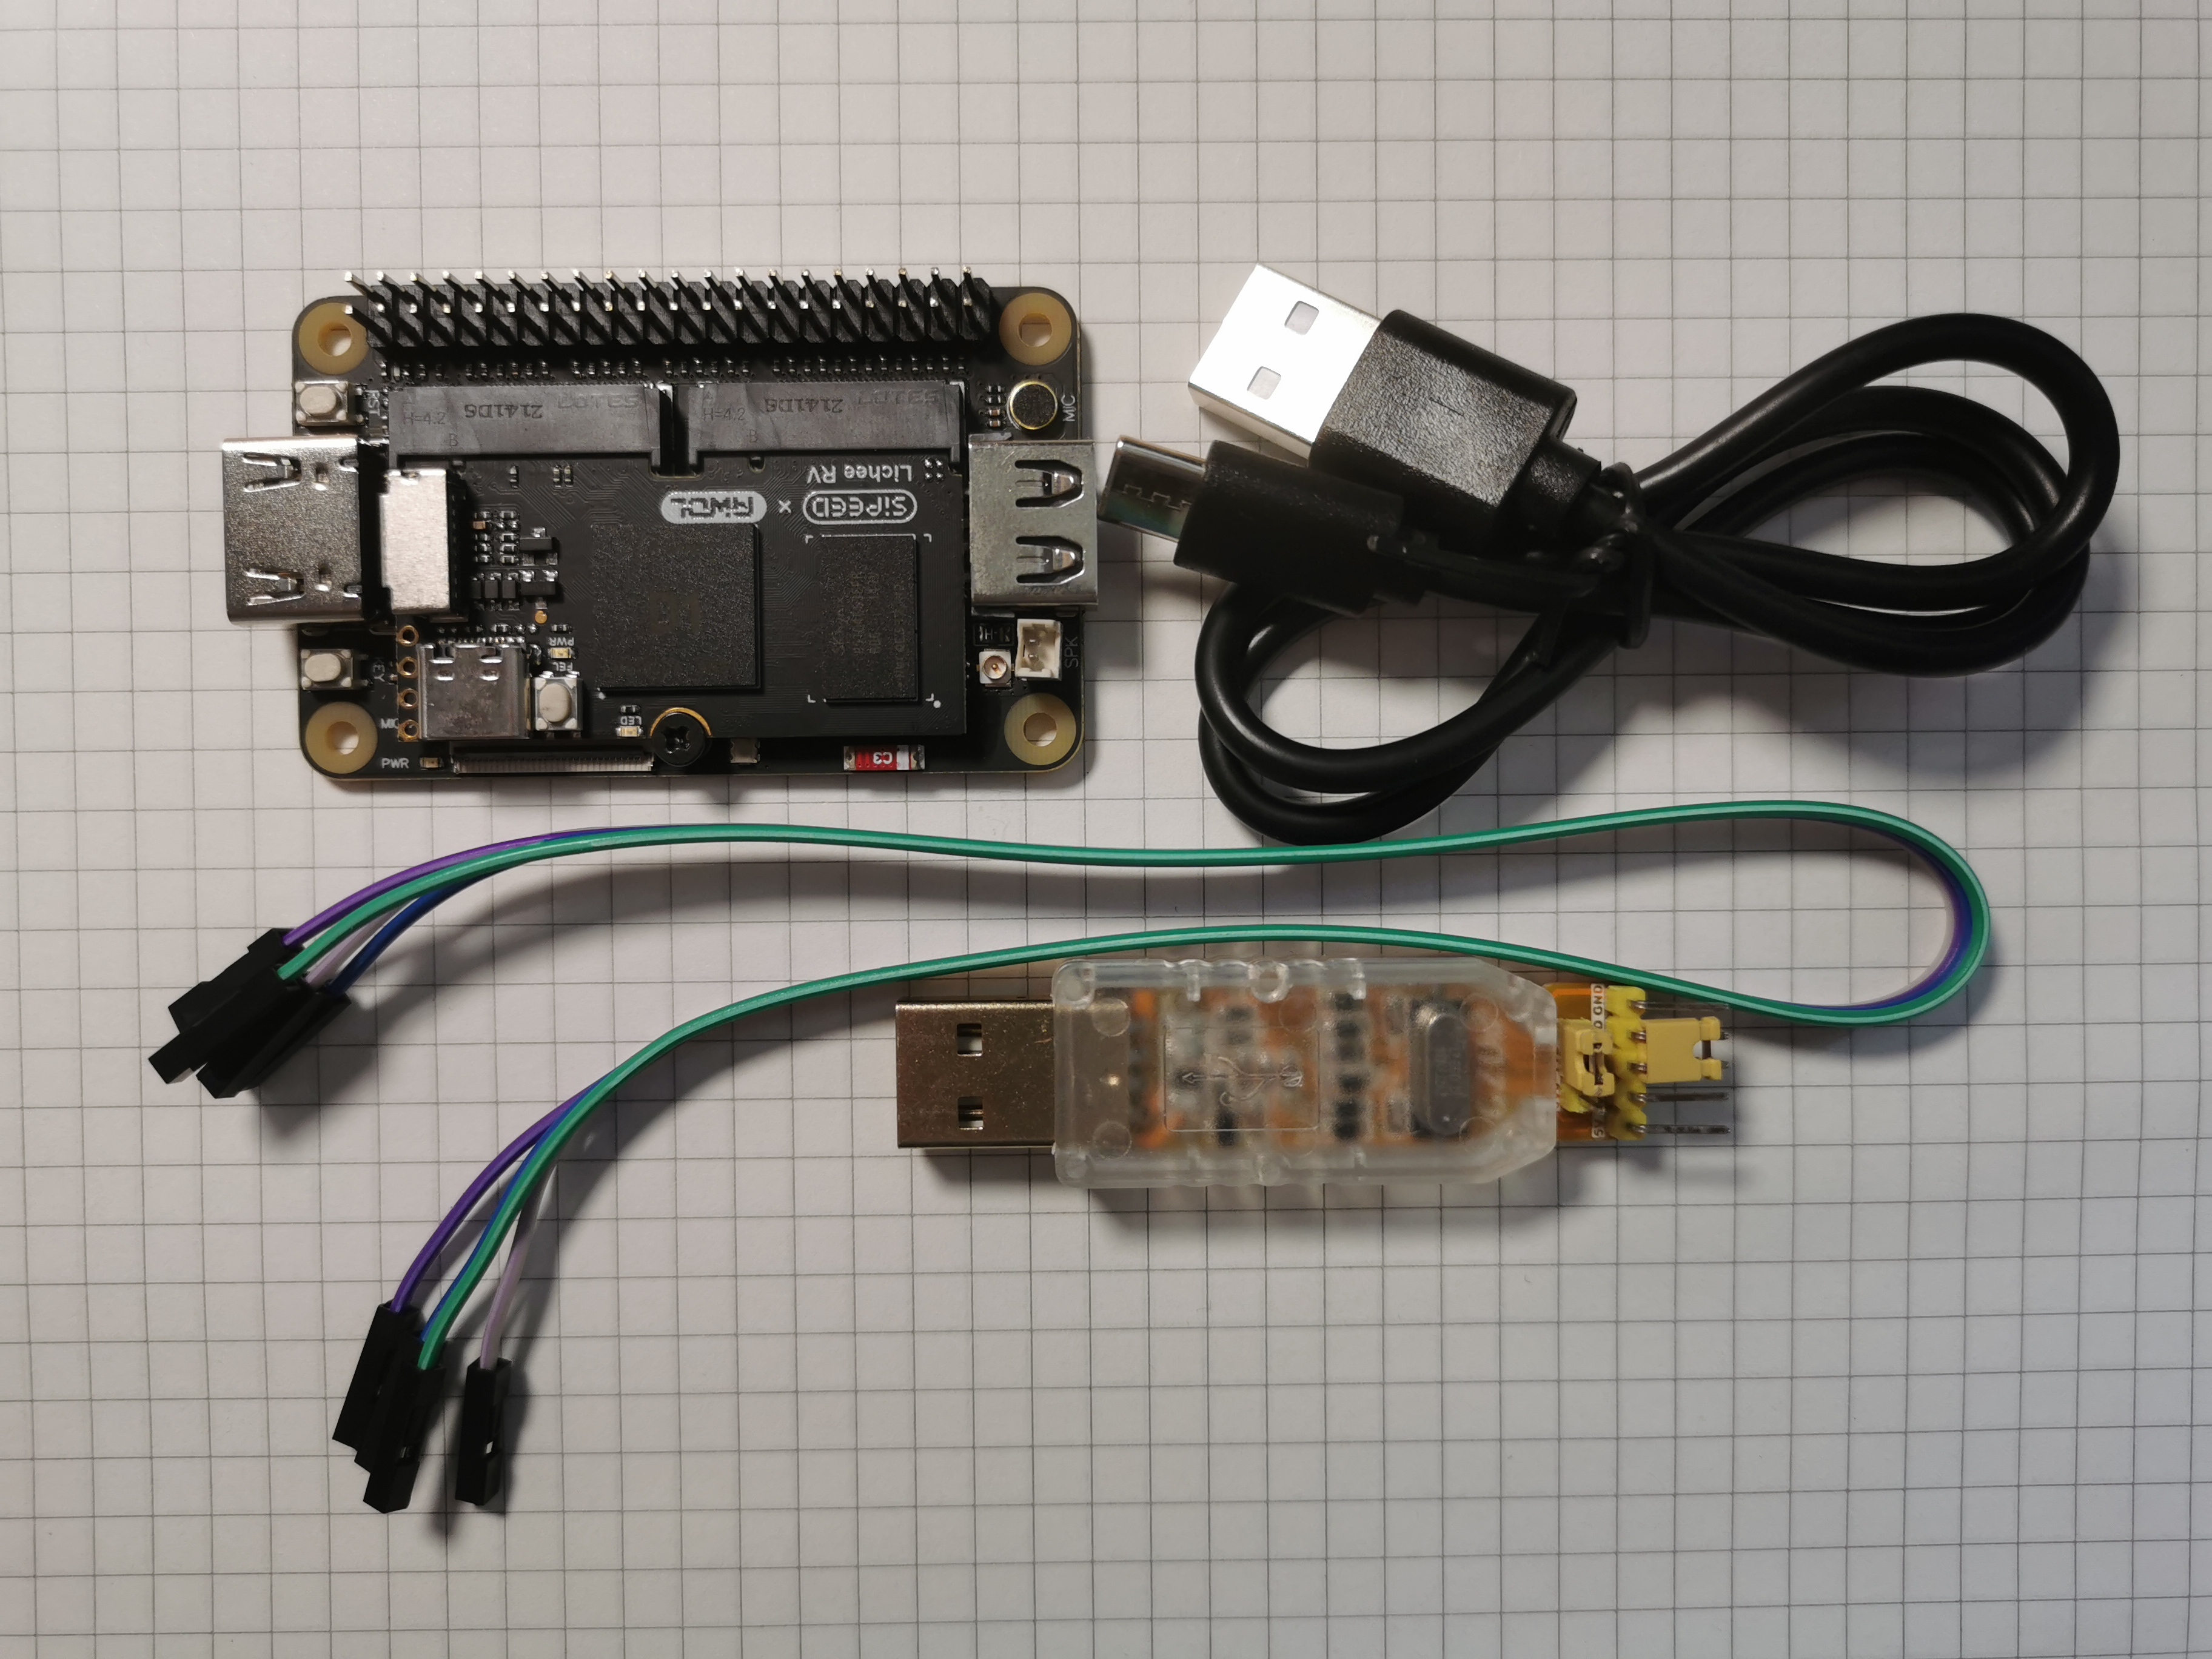
\includegraphics[width=0.7\textwidth]{RV_Kit.jpg}
  \caption{ 需要用到的硬件设备 }
\end{figure}

准备好这些设备后,使用 USB C 线将开发板连接到电脑,然后按一下开发板上的 fel 按钮, fel 按钮的位置在下图绿色LED灯上方的红框中:

\begin{figure}[H]
    \centering
    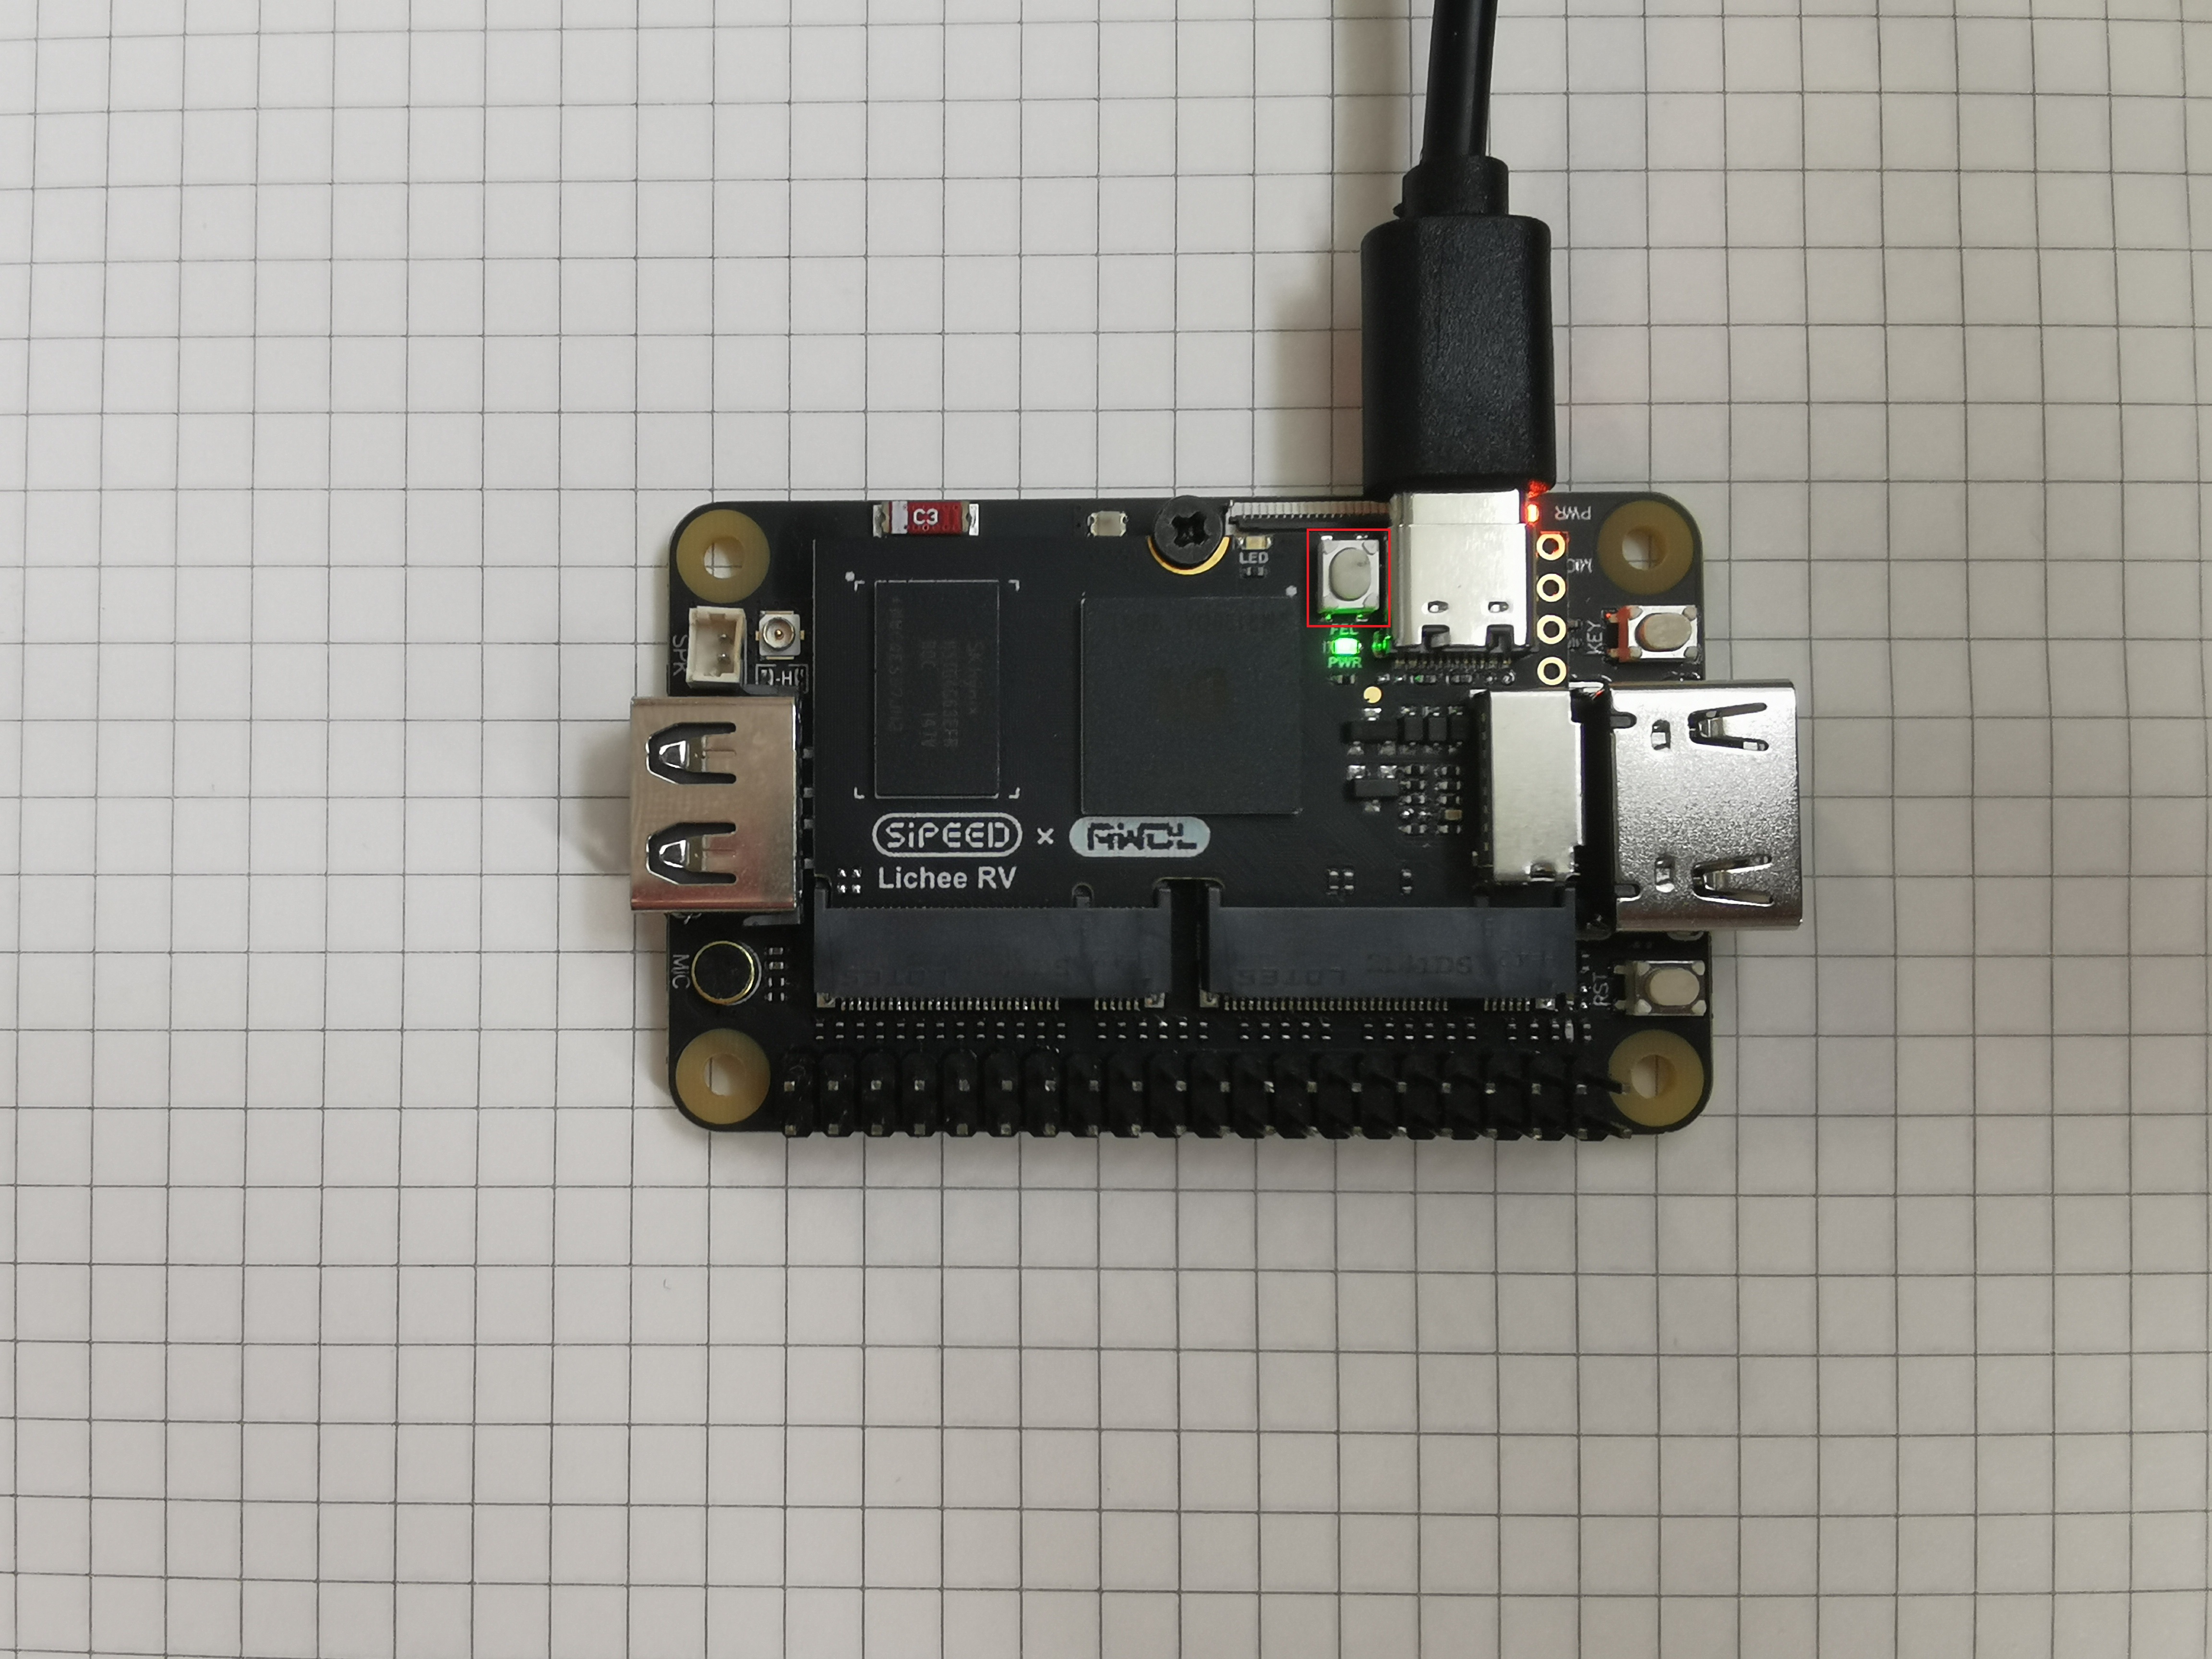
\includegraphics[width=0.8\textwidth]{RV_xfel1.jpg}
    \caption{ 测试开发板与 \lstinline{xfel} 的配置(1) }
\end{figure}

然后在终端中执行 \lstinline{xfel version} ,若出现类似下图所示的结果,即为 \lstinline{xfel} 正确识别开发板,开发板与 \lstinline{xfel} 的配置正确:
\begin{figure}[H]
    \centering
    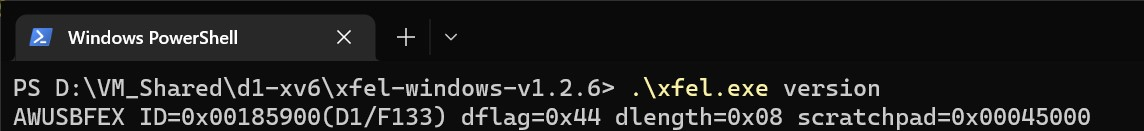
\includegraphics[width=0.7\textwidth]{RV_xfel2.jpg}
    \caption{ 测试开发板与 \lstinline{xfel} 的配置(2) }
\end{figure}

如果无法识别,则需要重新按下开发板上的 fel 按钮。由于不同批次的硬件的差异,上述结果可能略有不同,但大致上都会有诸如 \lstinline{D1/F133} 之类的字样出现。

\subsection{修改 xv6 代码}
这里大致说明一下修改代码的步骤,具体与原版 xv6 的不同点可以查看 \href{https://github.com/jwyjohn/xv6-riscv/commit/54745c4f7eea4af81f8e044953119ad81cd6822b#diff-c53dc675dd68c013f3e29c34d517877d7da3a48af39fe77b7b9541751aed722c}{这个diff} 的结果。

1. 将 xv6 移植到真实的硬件上时,第一个遇到的问题就是硬件的初始化问题。好在初始化时钟和硬件的代码已经有人写好\footnote{见 \url{https://github.com/bigmagic123/d1-nezha-baremeta}},我们拿来后(主要是 \lstinline{clk.c} 和 \lstinline{uartinit.c})略作修改就可以放入 xv6 的源码库中。

2. 为适配 Lichee RV,原来的 CLINT, PLIC, UART, UART IRQ 的地址按需修改,并且需要修改链接器脚本 \lstinline{kernel.ld} 使得内核的开始地址改为 \lstinline{0x40000000} 。

3. 由于 D1 具有物理内存保护机制(Physical Memory Protection (PMP)),相比于 qemu 虚拟机而言,需要初始化 PMP 才能成功地从 M 态切换到 S 态。

4. 由于该开发板的公司没有开源的 SD 卡驱动,故而我们使用内存盘模拟硬盘,而非使用 qemu 的 \lstinline{virtio}。

5. 对应的 Makefile 等配置也进行了修改,以方便将 \lstinline{fs.img} 链接入二进制的 \lstinline{kernel}。

\subsection{在开发板上启动 xv6 }

首先,使用 CH341 通过杜邦线连接到开发板的uart针脚,如下图所示:

\begin{figure}[H]
    \centering
    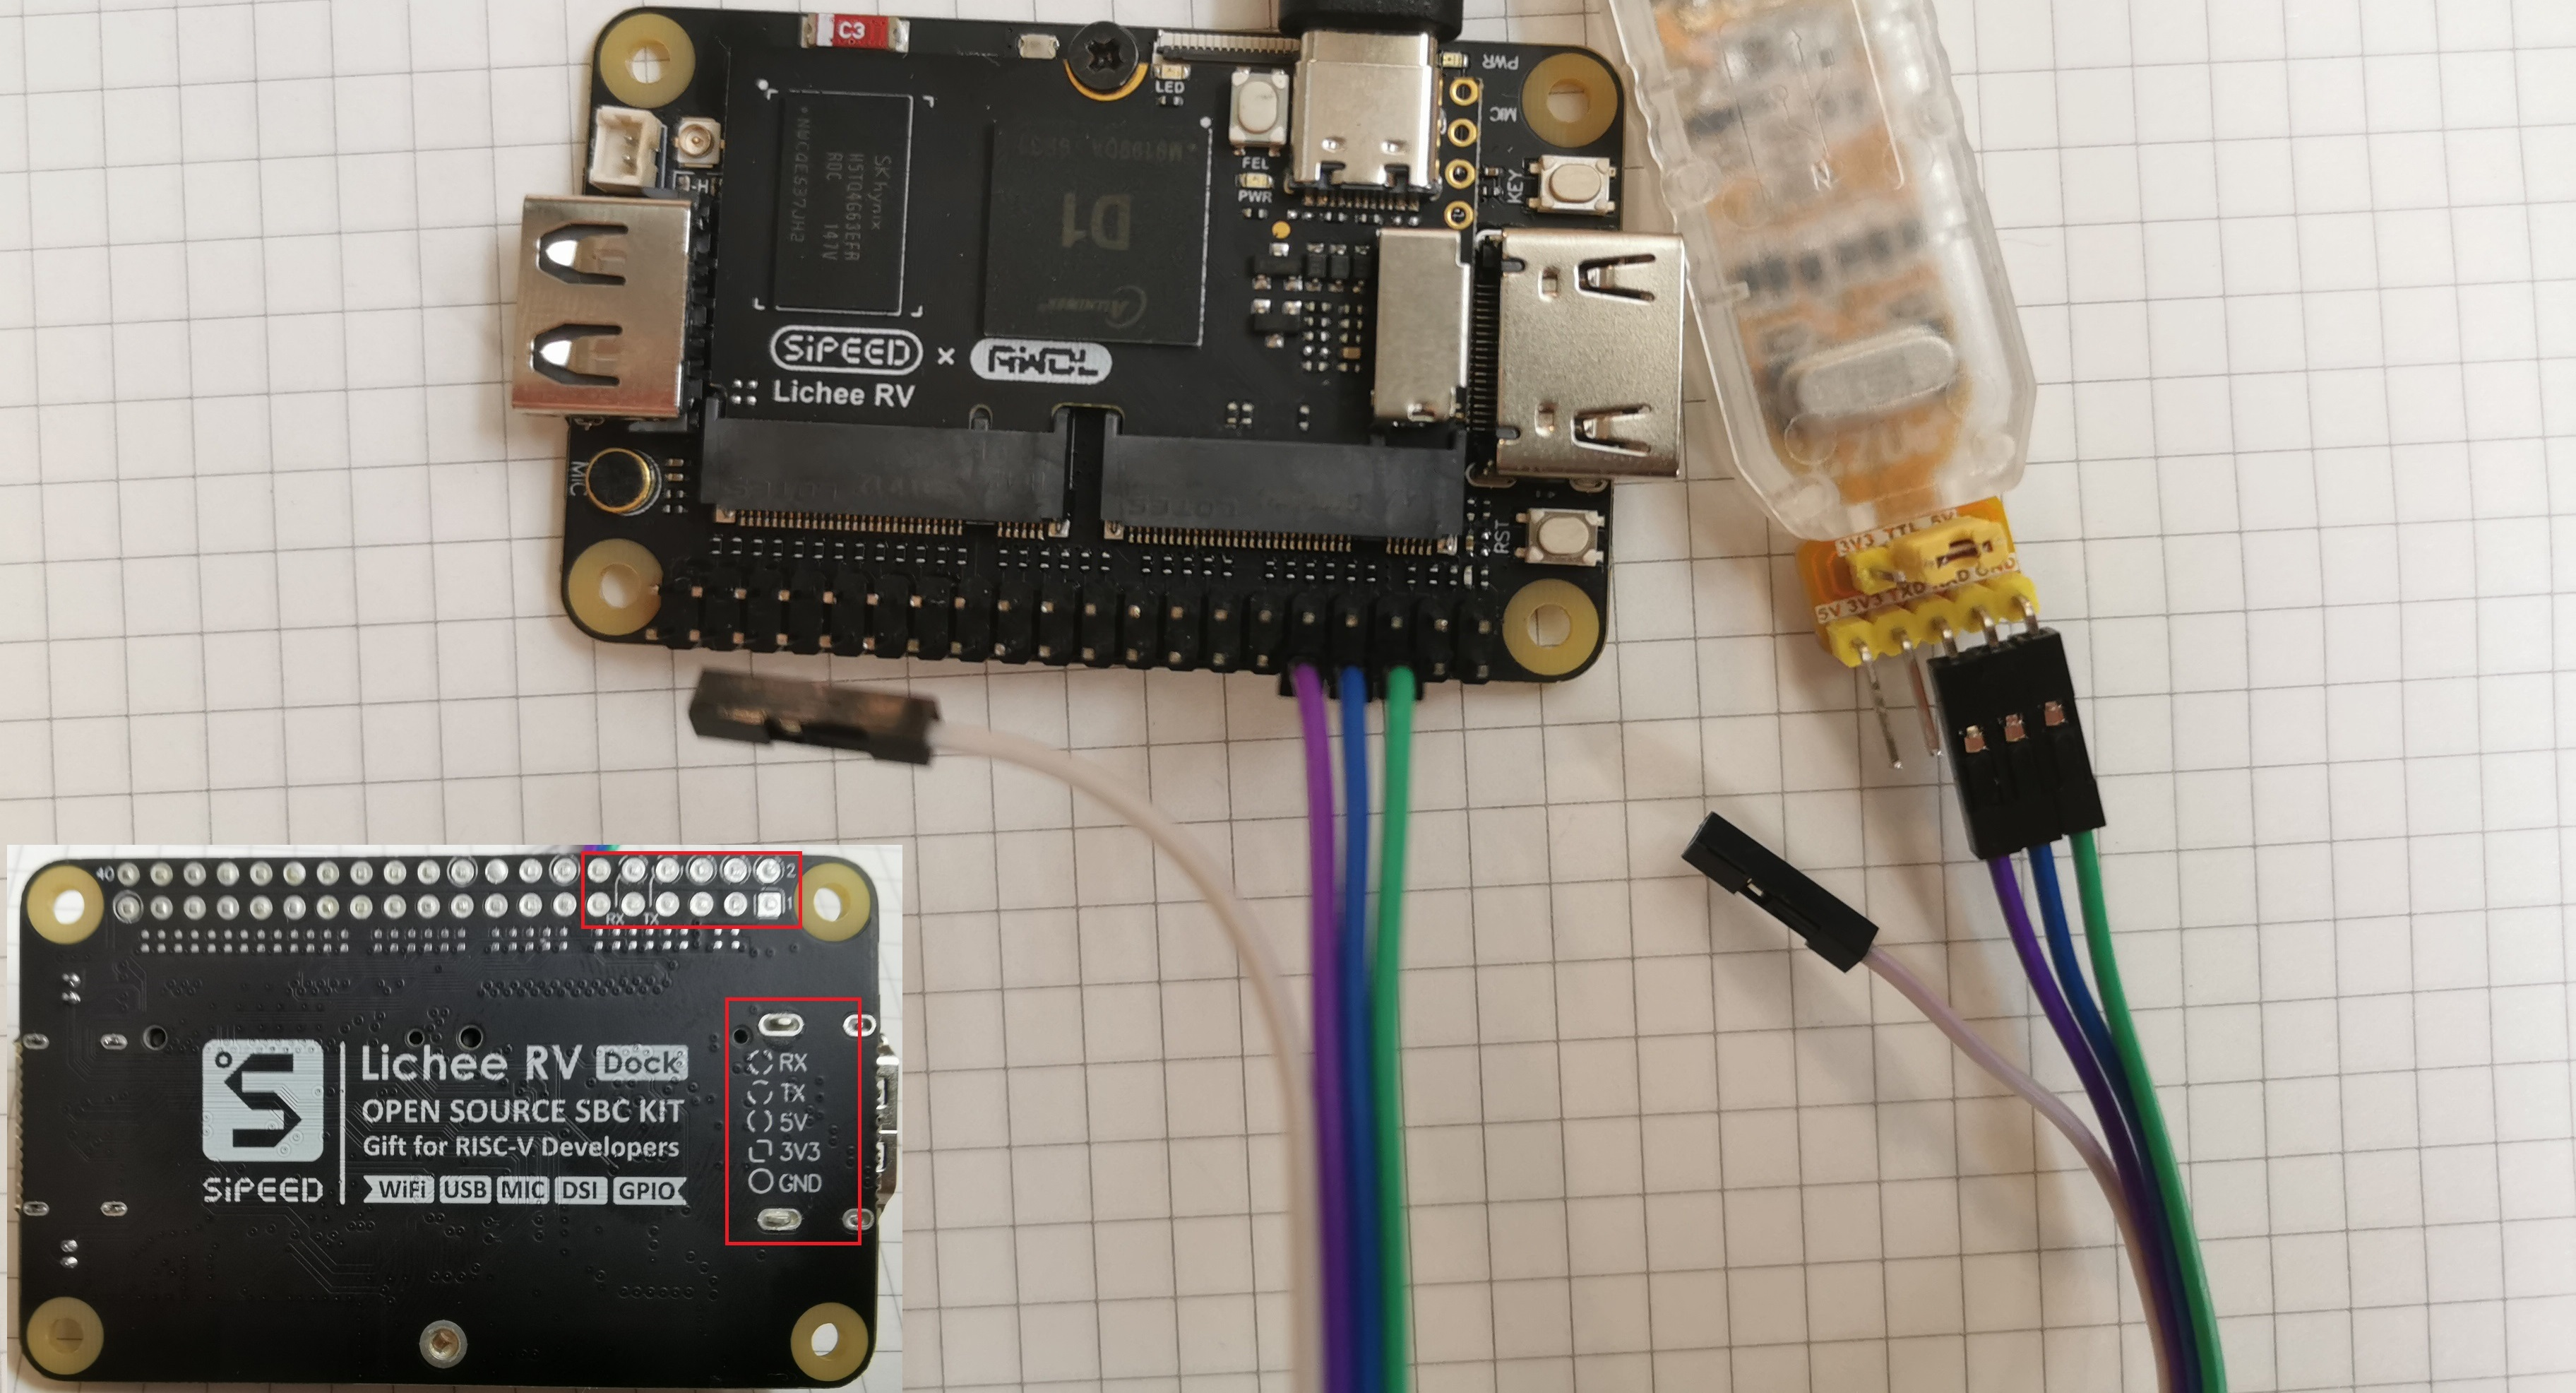
\includegraphics[width=0.7\textwidth]{RV_uart.jpg}
    \caption{ 开发板连接 uart 的线序(见左下红框中图示)}
\end{figure}

然后编译 xv6 的内核镜像,使用 \lstinline{make fs.img && make},成功后生成二进制文件 \lstinline{kernel/kernel.bin},将该文件拷贝到 \lstinline{xfel} 的目录下。

完成编译后,使用 USB C 线将开发板连接到电脑,然后按一下开发板上的 fel 按钮,然后再将接有杜邦线的 CH341 连接至电脑。

此时在终端中执行 \lstinline{xfel version} 确认开发板连接无误;然后在终端中执行 \lstinline{xfel ddr d1} 用于初始化开发板的内存控制器;然后使用 \lstinline{xfel write 0x40000000 ./kernel.bin} 将编译好的内核拷贝到内存中。

此时打开 Putty (或其它串口终端工具),设置波特率为 115200 ,然后打开 CH341 对应的 COM 口。最后在(原来执行xfel的)终端中执行 \lstinline{xfel exec 0x40000000},即可在 Putty 中看到 xv6 的启动信息,过程如下图所示:

\begin{figure}[H]
    \centering
    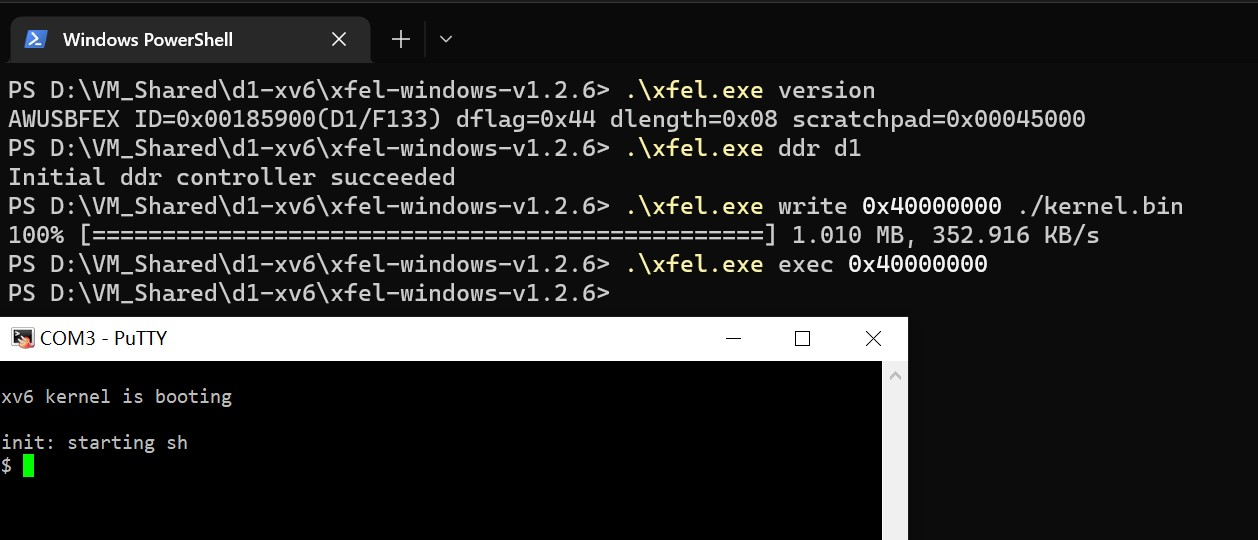
\includegraphics[width=0.7\textwidth]{RV_boot.jpg}
    \caption{ 在 Lichee RV 上启动 xv6}
\end{figure}

\begin{theorem}[Putty串口终端换行不正确]
    如果在连接开发板后,能够看到大概的输出,但是换行等格式较为混乱,则考虑在Putty的Terminal选项中勾选 Implicit CR in every LF 和 Implicit LF in every CR ,并将 Local echo 和 Local line editing 均设为 Force ,即可解决该问题。
\end{theorem}

可见在 Lichee RV 上成功启动 xv6 。下面尝试运行 \lstinline{usertests},结果如下图所示:

\begin{figure}[H]
    \centering
    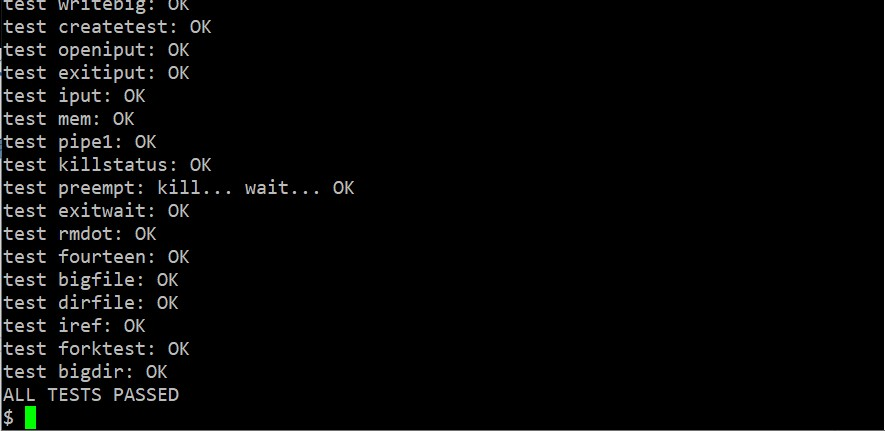
\includegraphics[width=0.7\textwidth]{RV_usertests.jpg}
    \caption{ 在 Lichee RV 上运行 \lstinline{usertests}}
\end{figure}

可见测试全部通过,说明我们在 Lichee RV 上运行 xv6 是成功的。

\section{给 xv6 增加一个应用编程语言}

能够在真实的硬件上跑 xv6 后,我们希望能够在 xv6 上提供给用户一个简易的开发环境,使其能够编写自己的用户态程序。由于类似 GCC 等工业级别的编译器的运行需要标准 C 语言库,而且其代码量巨大,移植较为困难,所以笔者选择了一种历史悠久、简单凝练但十分强大的语言 Scheme (一种 Lisp 方言\footnote{Lisp与Scheme的关系见:\url{https://en.wikipedia.org/wiki/Scheme_(programming_language)}第一段}),将其移植到原始的 xv6 环境中,从而使得 xv6 能成为可用的系统。

笔者选择移植的 Scheme 实现是由 Peter Michaux 实现的 Bootstrap Scheme\footnote{\url{https://github.com/petermichaux/bootstrap-scheme}}。 其本体仅由一个源文件构成,且依赖的标准 C 语言库中的内容十分少。

我们首先将其头文件更换为 xv6 提供的头文件:

\begin{lstlisting}[language=C]
// #include <stdlib.h>
// #include <stdio.h>
// #include <string.h>
// #include <ctype.h>

/**************************** FIXUP ******************************/
#include "kernel/types.h"
#include "user/user.h"
#include "kernel/fcntl.h"
#include <stdarg.h>
\end{lstlisting}

然后将输出的函数进行修改,以使其符合 xv6 用户C语言库的标准,在修改这些输出函数前,我们需要定义一些如\lstinline{stderr}的常量,以减少我们修改的工作量:
\begin{lstlisting}[language=C]
#define NULL 0
#define EOF 0
#define FD int

#define maxbufn 1024
#define maxfd 8

const int stdin = 0;
const int stdout = 1;
const int stderr = 2;
\end{lstlisting}

将所有的 \lstinline{fprintf}、\lstinline{open}、\lstinline{close} 等函数修改完成后,为了适应 xv6 中的 uart 串口中断,我们还需要实现几个常见的输入函数:
\begin{lstlisting}[language=C]

char ibuf[maxfd][maxbufn];
int bufptr[maxfd];
static char digits[] = "0123456789ABCDEF";

int getc(int fd)
{
  bufptr[fd]++;
  if (ibuf[fd][bufptr[fd]] == EOF || ibuf[fd][bufptr[fd]] == '\n' || ibuf[fd][bufptr[fd]] == '\r')
  {
    int i, cc;
    char c;
    bufptr[fd] = 0;
    for (i = 0; i + 1 < maxbufn;)
    {
      cc = read(fd, &c, 1);
      if (cc < 1)
        break;
      ibuf[fd][i++] = c;
      if (c == '\n' || c == '\r')
        break;
    }
  }
  int ret = ibuf[fd][bufptr[fd]];
  return ret;
}

void ungetc(char c, int fd)
{
  ibuf[fd][bufptr[fd]] = c;
  bufptr[fd]--;
}

void putc(char ch, int fd)
{
  ibuf[fd][++bufptr[fd]] = ch;
}

void fflush(int fd)
{
  ibuf[fd][++bufptr[fd]] = 0;
  fprintf(fd, ibuf[fd]);
  memset(ibuf[fd], 0x00, sizeof(ibuf[fd]));
  bufptr[fd] = 0;
}

void putchar(char c)
{
  printf("%c", c);
}

int isspace(char c) { return c == ' '; }
int isalpha(char c) { return (c >= 'a' && c <= 'z') || (c >= 'A' && c <= 'Z'); }
int isdigit(char c) { return (c >= '0' && c <= '9'); }
/**************************** MODEL ******************************/
\end{lstlisting}

将该源文件命名为 \lstinline{lisp.c} ,并将其加入到 Makefile 的用户程序中,继续修改细节直到通过编译。

\begin{theorem}[爆栈问题]
    通过编译后,在测试时发现,由于 xv6 的栈空间过小,故而导致其在使用递归函数时容易出现栈溢出的异常,进而修改 xv6 的 \lstinline{kernel/exec.c} 中的 \lstinline{exec()} 函数,增加其栈空间:
    \begin{lstlisting}[language=C]
        // Use the second as the user stack.
        int stack_pagenum = 1 + 1000;
        sz = PGROUNDUP(sz);
        uint64 sz1;
        if ((sz1 = uvmalloc(pagetable, sz, sz + stack_pagenum * PGSIZE)) == 0)
          goto bad;
        sz = sz1;
        uvmclear(pagetable, sz - stack_pagenum * PGSIZE);
        sp = sz;
        stackbase = sp - PGSIZE;
    \end{lstlisting}
    就可以缓解栈溢出的问题,要真正解决这个问题,需要在内核中实现栈内存动态分配的机制,相对较为繁琐。
\end{theorem}

进入 xv6 后,执行 \lstinline{lisp},就可以进入该编程语言的解释器,我们用如下的语句定义一个求 Fibonacci 数列的递归函数,然后试图求其第 15 项,如下图所示:

\begin{figure}[H]
    \centering
    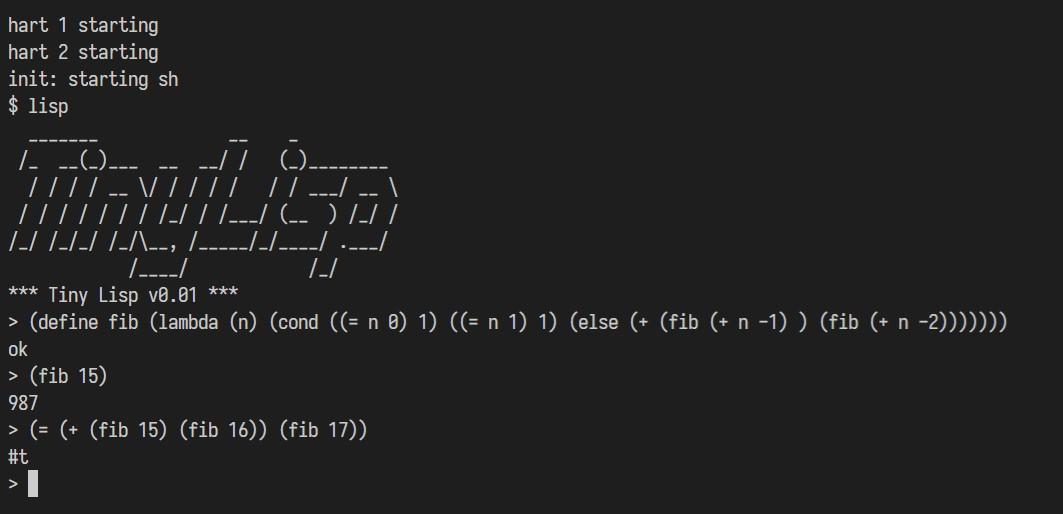
\includegraphics[width=0.7\textwidth]{RV_lisp.jpg}
    \caption{ 在 xv6 上使用 Scheme (Lisp) 编程求 Fibonacci 数列}
\end{figure}

可见程序运行符合预期,基本可以认为移植成功。

\section{更多后续的计划}

事实上,MIT 带给我们的 xv6 还有大量可以开发的潜力,下面列举笔者看到的一些比较有趣的关于 xv6 的开发计划:
\begin{enumerate}
    \item 使用 Rust 重写 xv6 (来自清华大学的项目)
    \item 将 xv6 移植到龙芯/MIPS架构上 (我校某同学的计划)
    \item 为 xv6 实现标准C语言库 (GitHub用户jahzielv的项目)
    \item 为 xv6 实现内核模块加载、卸载机制 (我校某同学的计划)
    \item 待续......
\end{enumerate}

\backmatter

\chapter{致谢}

在完成操作系统课程设计后,此笔者首先要感谢 MIT 提供的精彩的材料,虽然已经完成项目,但笔者感觉这份材料还是如《列子.汤问》所言:既去而余音绕梁檷,三日不绝,左右以其人弗去。

~\\

笔者也要感谢提供学费和生活上支持的父母,没有他们的帮助,笔者很难在短短一周时间内集中精力完成课设的实验。

~\\

短短的一周时间完成的实验和笔记,难免有所疏忽,望读者斧正。



\end{document}
